% Options for packages loaded elsewhere
\PassOptionsToPackage{unicode}{hyperref}
\PassOptionsToPackage{hyphens}{url}
\PassOptionsToPackage{dvipsnames,svgnames,x11names}{xcolor}
%
\documentclass[
  11pt,
]{krantz}
\usepackage{amsmath,amssymb}
\usepackage{lmodern}
\usepackage{iftex}
\ifPDFTeX
  \usepackage[T1]{fontenc}
  \usepackage[utf8]{inputenc}
  \usepackage{textcomp} % provide euro and other symbols
\else % if luatex or xetex
  \usepackage{unicode-math}
  \defaultfontfeatures{Scale=MatchLowercase}
  \defaultfontfeatures[\rmfamily]{Ligatures=TeX,Scale=1}
  \setmonofont[Scale=0.775]{MesloLGS NF}
\fi
% Use upquote if available, for straight quotes in verbatim environments
\IfFileExists{upquote.sty}{\usepackage{upquote}}{}
\IfFileExists{microtype.sty}{% use microtype if available
  \usepackage[]{microtype}
  \UseMicrotypeSet[protrusion]{basicmath} % disable protrusion for tt fonts
}{}
\makeatletter
\@ifundefined{KOMAClassName}{% if non-KOMA class
  \IfFileExists{parskip.sty}{%
    \usepackage{parskip}
  }{% else
    \setlength{\parindent}{0pt}
    \setlength{\parskip}{6pt plus 2pt minus 1pt}}
}{% if KOMA class
  \KOMAoptions{parskip=half}}
\makeatother
\usepackage{xcolor}
\IfFileExists{xurl.sty}{\usepackage{xurl}}{} % add URL line breaks if available
\IfFileExists{bookmark.sty}{\usepackage{bookmark}}{\usepackage{hyperref}}
\hypersetup{
  pdftitle={Data Science per psicologi},
  pdfauthor={Corrado Caudek},
  colorlinks=true,
  linkcolor={Maroon},
  filecolor={Maroon},
  citecolor={Blue},
  urlcolor={Blue},
  pdfcreator={LaTeX via pandoc}}
\urlstyle{same} % disable monospaced font for URLs
\usepackage{color}
\usepackage{fancyvrb}
\newcommand{\VerbBar}{|}
\newcommand{\VERB}{\Verb[commandchars=\\\{\}]}
\DefineVerbatimEnvironment{Highlighting}{Verbatim}{commandchars=\\\{\}}
% Add ',fontsize=\small' for more characters per line
\usepackage{framed}
\definecolor{shadecolor}{RGB}{248,248,248}
\newenvironment{Shaded}{\begin{snugshade}}{\end{snugshade}}
\newcommand{\AlertTok}[1]{\textcolor[rgb]{0.33,0.33,0.33}{#1}}
\newcommand{\AnnotationTok}[1]{\textcolor[rgb]{0.37,0.37,0.37}{\textbf{\textit{#1}}}}
\newcommand{\AttributeTok}[1]{\textcolor[rgb]{0.61,0.61,0.61}{#1}}
\newcommand{\BaseNTok}[1]{\textcolor[rgb]{0.06,0.06,0.06}{#1}}
\newcommand{\BuiltInTok}[1]{#1}
\newcommand{\CharTok}[1]{\textcolor[rgb]{0.5,0.5,0.5}{#1}}
\newcommand{\CommentTok}[1]{\textcolor[rgb]{0.37,0.37,0.37}{\textit{#1}}}
\newcommand{\CommentVarTok}[1]{\textcolor[rgb]{0.37,0.37,0.37}{\textbf{\textit{#1}}}}
\newcommand{\ConstantTok}[1]{\textcolor[rgb]{0,0,0}{#1}}
\newcommand{\ControlFlowTok}[1]{\textcolor[rgb]{0.27,0.27,0.27}{\textbf{#1}}}
\newcommand{\DataTypeTok}[1]{\textcolor[rgb]{0.27,0.27,0.27}{#1}}
\newcommand{\DecValTok}[1]{\textcolor[rgb]{0.06,0.06,0.06}{#1}}
\newcommand{\DocumentationTok}[1]{\textcolor[rgb]{0.37,0.37,0.37}{\textbf{\textit{#1}}}}
\newcommand{\ErrorTok}[1]{\textcolor[rgb]{0.14,0.14,0.14}{\textbf{#1}}}
\newcommand{\ExtensionTok}[1]{#1}
\newcommand{\FloatTok}[1]{\textcolor[rgb]{0.06,0.06,0.06}{#1}}
\newcommand{\FunctionTok}[1]{\textcolor[rgb]{0,0,0}{#1}}
\newcommand{\ImportTok}[1]{#1}
\newcommand{\InformationTok}[1]{\textcolor[rgb]{0.37,0.37,0.37}{\textbf{\textit{#1}}}}
\newcommand{\KeywordTok}[1]{\textcolor[rgb]{0.27,0.27,0.27}{\textbf{#1}}}
\newcommand{\NormalTok}[1]{#1}
\newcommand{\OperatorTok}[1]{\textcolor[rgb]{0.43,0.43,0.43}{\textbf{#1}}}
\newcommand{\OtherTok}[1]{\textcolor[rgb]{0.37,0.37,0.37}{#1}}
\newcommand{\PreprocessorTok}[1]{\textcolor[rgb]{0.37,0.37,0.37}{\textit{#1}}}
\newcommand{\RegionMarkerTok}[1]{#1}
\newcommand{\SpecialCharTok}[1]{\textcolor[rgb]{0,0,0}{#1}}
\newcommand{\SpecialStringTok}[1]{\textcolor[rgb]{0.5,0.5,0.5}{#1}}
\newcommand{\StringTok}[1]{\textcolor[rgb]{0.5,0.5,0.5}{#1}}
\newcommand{\VariableTok}[1]{\textcolor[rgb]{0,0,0}{#1}}
\newcommand{\VerbatimStringTok}[1]{\textcolor[rgb]{0.5,0.5,0.5}{#1}}
\newcommand{\WarningTok}[1]{\textcolor[rgb]{0.37,0.37,0.37}{\textbf{\textit{#1}}}}
\usepackage{longtable,booktabs,array}
\usepackage{calc} % for calculating minipage widths
% Correct order of tables after \paragraph or \subparagraph
\usepackage{etoolbox}
\makeatletter
\patchcmd\longtable{\par}{\if@noskipsec\mbox{}\fi\par}{}{}
\makeatother
% Allow footnotes in longtable head/foot
\IfFileExists{footnotehyper.sty}{\usepackage{footnotehyper}}{\usepackage{footnote}}
\makesavenoteenv{longtable}
\usepackage{graphicx}
\makeatletter
\def\maxwidth{\ifdim\Gin@nat@width>\linewidth\linewidth\else\Gin@nat@width\fi}
\def\maxheight{\ifdim\Gin@nat@height>\textheight\textheight\else\Gin@nat@height\fi}
\makeatother
% Scale images if necessary, so that they will not overflow the page
% margins by default, and it is still possible to overwrite the defaults
% using explicit options in \includegraphics[width, height, ...]{}
\setkeys{Gin}{width=\maxwidth,height=\maxheight,keepaspectratio}
% Set default figure placement to htbp
\makeatletter
\def\fps@figure{htbp}
\makeatother
\setlength{\emergencystretch}{3em} % prevent overfull lines
\providecommand{\tightlist}{%
  \setlength{\itemsep}{0pt}\setlength{\parskip}{0pt}}
\setcounter{secnumdepth}{5}
\defaultfontfeatures{Scale=MatchLowercase}

\usepackage{booktabs}
\usepackage{longtable}
\usepackage[bf,singlelinecheck=off]{caption}

\usepackage{framed,color}
\definecolor{shadecolor}{RGB}{248,248,248}

\renewcommand{\textfraction}{0.05}
\renewcommand{\topfraction}{0.8}
\renewcommand{\bottomfraction}{0.8}
\renewcommand{\floatpagefraction}{0.75}

\renewenvironment{quote}{\begin{VF}}{\end{VF}}
\let\oldhref\href
\renewcommand{\href}[2]{#2\footnote{\url{#1}}}

\ifxetex
  \usepackage{letltxmacro}
  \setlength{\XeTeXLinkMargin}{1pt}
  \LetLtxMacro\SavedIncludeGraphics\includegraphics
  \def\includegraphics#1#{% #1 catches optional stuff (star/opt. arg.)
    \IncludeGraphicsAux{#1}%
  }%
  \newcommand*{\IncludeGraphicsAux}[2]{%
    \XeTeXLinkBox{%
      \SavedIncludeGraphics#1{#2}%
    }%
  }%
\fi

\makeatletter
\newenvironment{kframe}{%
\medskip{}
\setlength{\fboxsep}{.8em}
 \def\at@end@of@kframe{}%
 \ifinner\ifhmode%
  \def\at@end@of@kframe{\end{minipage}}%
  \begin{minipage}{\columnwidth}%
 \fi\fi%
 \def\FrameCommand##1{\hskip\@totalleftmargin \hskip-\fboxsep
 \colorbox{shadecolor}{##1}\hskip-\fboxsep
     % There is no \\@totalrightmargin, so:
     \hskip-\linewidth \hskip-\@totalleftmargin \hskip\columnwidth}%
 \MakeFramed {\advance\hsize-\width
   \@totalleftmargin\z@ \linewidth\hsize
   \@setminipage}}%
 {\par\unskip\endMakeFramed%
 \at@end@of@kframe}
\makeatother

\renewenvironment{Shaded}{\begin{kframe}}{\end{kframe}}

\usepackage{makeidx}
\makeindex

\urlstyle{tt}

\usepackage{amsthm}
\makeatletter
\def\thm@space@setup{%
  \thm@preskip=8pt plus 2pt minus 4pt
  \thm@postskip=\thm@preskip
}
\makeatother

\newcommand{\E}{\mathbb{E}} % Define expected value operator
\DeclareMathOperator{\Var}{\mathbb{V}} % Define variance operator
\DeclareMathOperator{\SD}{SD} % Define sd operator
\DeclareMathOperator{\Cov}{Cov} % Define covariance operator
\DeclareMathOperator{\Corr}{Corr} % Define correlation operator
\DeclareMathOperator{\Me}{Me} % Define mediane operator
\DeclareMathOperator{\Mo}{Mo} % Define mode operator
\DeclareMathOperator{\Bin}{Bin} % Define binomial operator
\DeclareMathOperator{\Bernoulli}{Bernoulli} % Define Bernoulli operator
\DeclareMathOperator{\Poi}{Poi} % Define Poisson operator
\DeclareMathOperator{\Uniform}{Uniform} % Define Uniform operator
\DeclareMathOperator{\Cauchy}{Cauchy} % Define Cauchy operator
\DeclareMathOperator{\elpd}{elpd} % Define elpd operator
\DeclareMathOperator{\lppd}{lppd} % Define lppd operator
\DeclareMathOperator{\LOO}{LOO} % Define LOO operator
\DeclareMathOperator{\Ber}{\mathscr{B}} % Define Bernoulli operator
\DeclareMathOperator{\B}{B} % beta function
% \mbox{B}(a, b) % beta function
% \mbox{Beta}(a, b) % beta distribution
\newcommand{\R}{\textsf{R}} % Define R programming language symbol
\newcommand{\Real}{\mathbb{R}} % Define real number operator
\newcommand{\Prob}{\mathscr{P}}
\newcommand{\indep}{\perp \!\!\! \perp}
\DeclareMathOperator{\argmin}{arg\,min} % thin space, limits on side in displays
\DeclareMathOperator{\argmax}{arg\,max} % no space, limits on side in displays

\raggedbottom % allow variable (ragged) site heights
\frenchspacing

\usepackage[
 labelfont=bf,
 font={small, it}
]{caption}
\usepackage{upquote} % print correct quotes in verbatim-environments
\usepackage{empheq}
\usepackage{xfrac}

\usepackage{polyglossia}
\setmainlanguage{italian}

% \DeclareMathSizes{10}{9}{7}{5}

\frontmatter
\ifLuaTeX
  \usepackage{selnolig}  % disable illegal ligatures
\fi
\usepackage[]{natbib}
\bibliographystyle{apalike}

\title{Data Science per psicologi}
\author{Corrado Caudek}
\date{2022-01-24}

\usepackage{amsthm}
\newtheorem{theorem}{Teorema}[chapter]
\newtheorem{lemma}{Lemma}[chapter]
\newtheorem{corollary}{Corollario}[chapter]
\newtheorem{proposition}{Proposizione}[chapter]
\newtheorem{conjecture}{Congettura}[chapter]
\theoremstyle{definition}
\newtheorem{definition}{Definizione}[chapter]
\theoremstyle{definition}
\newtheorem{example}{Esempio}[chapter]
\theoremstyle{definition}
\newtheorem{exercise}{Esercizio}[chapter]
\theoremstyle{definition}
\newtheorem{hypothesis}{Hypothesis}[chapter]
\theoremstyle{remark}
\newtheorem*{remark}{Osservazione}
\newtheorem*{solution}{Soluzione}
\begin{document}
\maketitle

\cleardoublepage\newpage\thispagestyle{empty}\null
% \cleardoublepage\newpage\thispagestyle{empty}\null
%\cleardoublepage\newpage
\thispagestyle{empty}
\begin{center}
\Large{Psicometria -- AA 2021/2022}

\vskip20pt

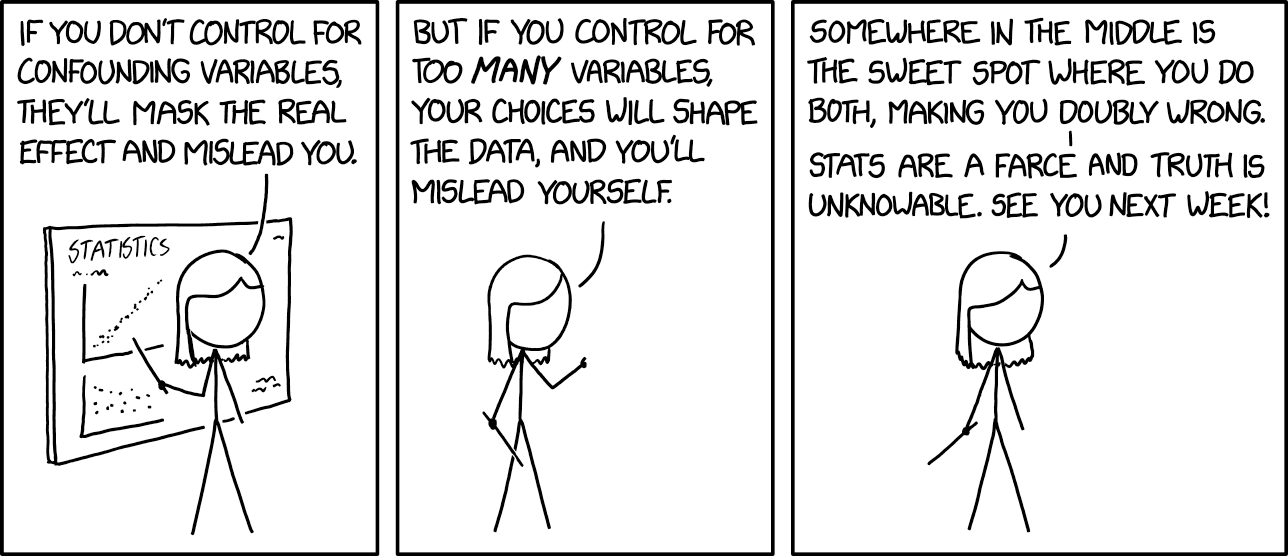
\includegraphics{images/confounding_variables.png}
\end{center}

\setlength{\abovedisplayskip}{-5pt}
\setlength{\abovedisplayshortskip}{-5pt}

{
\hypersetup{linkcolor=}
\setcounter{tocdepth}{2}
\tableofcontents
}
\listoffigures
\listoftables
\hypertarget{prefazione}{%
\chapter*{Prefazione}\label{prefazione}}


\emph{Data Science per psicologi} contiene il materiale delle lezioni dell'insegnamento di \emph{Psicometria B000286} (A.A. 2021/2022) rivolto agli studenti del primo anno del Corso di Laurea in Scienze e Tecniche Psicologiche dell'Università degli Studi di Firenze. \emph{Psicometria} si propone di fornire agli studenti un'introduzione all'analisi dei dati in psicologia. Le conoscenze/competenze che verranno sviluppate in questo insegnamento sono quelle della Data science, ovvero un insieme di conoscenze/competenze che si pongono all'intersezione tra statistica (ovvero, richiedono la capacità di comprendere teoremi statistici) e informatica (ovvero, richiedono la capacità di sapere utilizzare un software).

\hypertarget{la-psicologia-e-la-data-science}{%
\section*{La psicologia e la Data science}\label{la-psicologia-e-la-data-science}}


Sembra sensato spendere due parole su un tema che è importante per gli studenti: quello indicato dal titolo di questo Capitolo. È ovvio che agli studenti di psicologia la statistica non piace. Se piacesse, forse studierebbero Data science e non psicologia; ma non lo fanno. Di conseguenza, gli studenti di psicologia si chiedono: ``perché dobbiamo perdere tanto tempo a studiare queste cose quando in realtà quello che ci interessa è tutt'altro?'' Questa è una bella domanda.

C'è una ragione molto semplice che dovrebbe farci capire perché la Data science è così importante per la psicologia. Infatti, a ben pensarci, la psicologia è una disciplina intrinsecamente statistica, se per statistica intendiamo quella disciplina che studia la variazione delle caratteristiche degli individui nella popolazione. La psicologia studia \emph{gli individui} ed è proprio la variabilità inter- e intra-individuale ciò che vogliamo descrivere e, in certi casi, predire. In questo senso, la psicologia è molto diversa dall'ingegneria, per esempio. Le proprietà di un determinato ponte sotto certe condizioni, ad esempio, sono molto simili a quelle di un altro ponte, sotto le medesime condizioni. Quindi, per un ingegnere la statistica è poco importante: le proprietà dei materiali sono unicamente dipendenti dalla loro composizione e restano costanti. Ma lo stesso non può dirsi degli individui: ogni individuo è unico e cambia nel tempo. E le variazioni tra gli individui, e di un individuo nel tempo, sono l'oggetto di studio proprio della psicologia: è dunque chiaro che i problemi che la psicologia si pone sono molto diversi da quelli affrontati, per esempio, dagli ingegneri. Questa è la ragione per cui abbiamo tanto bisogno della Data science in psicologia: perché la Data science ci consente di descrivere la variazione e il cambiamento. E queste sono appunto le caratteristiche di base dei fenomeni psicologici.

Sono sicuro che, leggendo queste righe, a molti studenti sarà venuta in mente la seguente domanda: perché non chiediamo a qualche esperto di fare il ``lavoro sporco'' (ovvero le analisi statistiche) per noi, mentre noi (gli psicologi) ci occupiamo solo di ciò che ci interessa, ovvero dei problemi psicologici slegati dai dettagli ``tecnici'' della Data science? La risposta a questa domanda è che non è possibile progettare uno studio psicologico sensato senza avere almeno una comprensione rudimentale della Data science. Le tematiche della Data science non possono essere ignorate né dai ricercatori in psicologia né da coloro che svolgono la professione di psicologo al di fuori dell'Università. Infatti, anche i professionisti al di fuori dall'università non possono fare a meno di leggere la letteratura psicologica più recente: il continuo aggiornamento delle conoscenze è infatti richiesto dalla deontologia della professione. Ma per potere fare questo è necessario conoscere un bel po' di Data science! Basta aprire a caso una rivista specialistica di psicologia per rendersi conto di quanto ciò sia vero: gli articoli che riportano i risultati delle ricerche psicologiche sono zeppi di analisi statistiche e di modelli formali. E la comprensione della letteratura psicologica rappresenta un requisito minimo nel bagaglio professionale dello psicologo.

Le considerazioni precedenti cercano di chiarire il seguente punto: la Data science non è qualcosa da studiare a malincuore, in un singolo insegnamento universitario, per poi poterla tranquillamente dimenticare. Nel bene e nel male, gli psicologi usano gli strumenti della Data science in tantissimi ambiti della loro attività professionale: in particolare quando costruiscono, somministrano e interpretano i test psicometrici. È dunque chiaro che possedere delle solide basi di Data science è un tassello imprescindibile del bagaglio professionale dello psicologo. In questo insegnamento verrano trattati i temi base della Data science e verrà adottato un punto di vista bayesiano, che corrisponde all'approccio più recente e sempre più diffuso in psicologia.

\hypertarget{come-studiare}{%
\section*{Come studiare}\label{come-studiare}}


Il giusto metodo di studio per prepararsi all'esame di Psicometria è quello di seguire attivamente le lezioni, assimilare i concetti via via che essi vengono presentati e verificare in autonomia le procedure presentate a lezione. Incoraggio gli studenti a farmi domande per chiarire ciò che non è stato capito appieno. Incoraggio gli studenti a utilizzare i forum attivi su Moodle e, soprattutto, a svolgere gli esercizi proposti su Moodle. I problemi forniti su Moodle rappresentano il livello di difficoltà richiesto per superare l'esame e consentono allo studente di comprendere se le competenze sviluppate fino a quel punto sono sufficienti rispetto alle richieste dell'esame.

La prima fase dello studio, che è sicuramente individuale, è quella in cui è necessario acquisire le conoscenze teoriche relative ai problemi che saranno presentati all'esame. La seconda fase di studio, che può essere facilitata da scambi con altri e da incontri di gruppo, porta ad acquisire la capacità di applicare le conoscenze: è necessario capire come usare un software (\(\textsf{R}\)) per applicare i concetti statistici alla specifica situazione del problema che si vuole risolvere. Le due fasi non sono però separate: il saper fare molto spesso ci aiuta a capire meglio.

\hypertarget{sviluppare-un-metodo-di-studio-efficace}{%
\section*{Sviluppare un metodo di studio efficace}\label{sviluppare-un-metodo-di-studio-efficace}}


Avendo insegnato molte volte in passato un corso introduttivo di analisi dei dati ho notato nel corso degli anni che gli studenti con l'atteggiamento mentale che descriverò qui sotto generalmente ottengono ottimi risultati. Alcuni studenti sviluppano naturalmente questo approccio allo studio, ma altri hanno bisogno di fare uno sforzo per maturarlo. Fornisco qui sotto una breve descrizione del ``metodo di studio'' che, nella mia esperienza, è il più efficace per affrontare le richieste di questo insegnamento.

\begin{itemize}
\tightlist
\item
  Dedicate un tempo sufficiente al materiale di base, apparentemente facile; assicuratevi di averlo capito bene. Cercate le lacune nella vostra comprensione. Leggere presentazioni diverse dello stesso materiale (in libri o articoli diversi) può fornire nuove intuizioni.
\item
  Gli errori che facciamo sono i nostri migliori maestri. Istintivamente cerchiamo di dimenticare subito i nostri errori. Ma il miglior modo di imparare è apprendere dagli errori che commettiamo. In questo senso, una soluzione corretta è meno utile di una soluzione sbagliata. Quando commettiamo un errore questo ci fornisce un'informazione importante: ci fa capire qual è il materiale di studio sul quale dobbiamo ritornare e che dobbiamo capire meglio.
\item
  C'è ovviamente un aspetto ``psicologico'' nello studio. Quando un esercizio o problema ci sembra incomprensibile, la cosa migliore da fare è dire: ``mi arrendo'', ``non ho idea di cosa fare!''. Questo ci rilassa: ci siamo già arresi, quindi non abbiamo niente da perdere, non dobbiamo più preoccuparci. Ma non dobbiamo fermarci qui. Le cose ``migliori'' che faccio (se ci sono) le faccio quando non ho voglia di lavorare. Alle volte, quando c'è qualcosa che non so fare e non ho idea di come affontare, mi dico: ``oggi non ho proprio voglia di fare fatica'', non ho voglia di mettermi nello stato mentale per cui ``in 10 minuti devo risolvere il problema perché dopo devo fare altre cose''. Però ho voglia di \emph{divertirmi} con quel problema e allora mi dedico a qualche aspetto ``marginale'' del problema, che so come affrontare, oppure considero l'aspetto più difficile del problema, quello che non so come risolvere, ma invece di cercare di risolverlo, guardo come altre persone hanno affrontato problemi simili, opppure lo stesso problema in un altro contesto. Non mi pongo l'obiettivo ``risolvi il problema in 10 minuti'', ma invece quello di farmi un'idea ``generale'' del problema, o quello di capire un caso più specifico e più semplice del problema. Senza nessuna pressione. Infatti, in quel momento ho deciso di non lavorare (ovvero, di non fare fatica). Va benissimo se ``parto per la tangente'', ovvero se mi metto a leggere del materiale che sembra avere poco a che fare con il problema centrale (le nostre intuizioni e la nostra curiosità solitamente ci indirizzano sulla strada giusta). Quando faccio così, molto spesso trovo la soluzione del problema che mi ero posto e, paradossalmente, la trovo in un tempo minore di quello che, in precedenza, avevo dedicato a ``lavorare'' al problema. Allora perché non faccio sempre così? C'è ovviamente l'aspetto dei ``10 minuti'' che non è sempre facile da dimenticare. Sotto pressione, possiamo solo agire in maniera automatica, ovvero possiamo solo applicare qualcosa che già sappiamo fare. Ma se dobbiamo imparare qualcosa di nuovo, la pressione è un impedimento.
\item
  È utile farsi da soli delle domande sugli argomenti trattati, senza limitarsi a cercare di risolvere gli esercizi che vengono assegnati. Quando studio qualcosa mi viene in mente: ``se questo è vero, allora deve succedere quest'altra cosa''. Allora verifico se questo è vero, di solito con una simulazione. Se i risultati della simulazione sono quelli che mi aspetto, allora vuol dire che ho capito. Se i risultati sono diversi da quelli che mi aspettavo, allora mi rendo conto di non avere capito e ritorno indietro a studiare con più attenzione la teoria che pensavo di avere capito -- e ovviamente mi rendo conto che c'era un aspetto che avevo frainteso. Questo tipo di verifica è qualcosa che dobbiamo fare da soli, in prima persona: nessun altro può fare questo al posto nostro.
\item
  Non aspettatevi di capire tutto la prima volta che incontrate un argomento nuovo.\footnote{Ricordatevi inoltre che gli individui tendono a sottostimare la propria capacità di apprendere \citep{horn2021underestimating}.} È utile farsi una nota mentalmente delle lacune nella vostra comprensione e tornare su di esse in seguito per carcare di colmarle. L'atteggiamento naturale, quando non capiamo i dettagli di qualcosa, è quello di pensare: ``non importa, ho capito in maniera approssimativa questo punto, non devo preoccuparmi del resto''. Ma in realtà non è vero: se la nostra comprensione è superficiale, quando il problema verrà presentato in una nuova forma, non riusciremo a risolverlo. Per cui i dubbi che ci vengono quando studiamo qualcosa sono il nostro alleato più prezioso: ci dicono esattamente quali sono gli aspetti che dobbiamo approfondire per potere migliorare la nostra preparazione.
\item
  È utile sviluppare una visione d'insieme degli argomenti trattati, capire l'obiettivo generale che si vuole raggiungere e avere chiaro il contributo che i vari pezzi di informazione forniscono al raggiungimento di tale obiettivo. Questa organizzazione mentale del materiale di studio facilita la comprensione. È estremamente utile creare degli schemi di ciò che si sta studiando. Non aspettate che sia io a fornirvi un riepilogo di ciò che dovete imparare: sviluppate da soli tali schemi e tali riassunti.
\item
  Tutti noi dobbiamo imparare l'arte di trovare le informazioni, non solo nel caso di questo insegnamento. Quando vi trovate di fronte a qualcosa che non capite, o ottenete un oscuro messaggio di errore da un software, ricordatevi: ``Google is your friend''!
\end{itemize}

\begin{flushright}
Corrado Caudek\\
Marzo 2022 \end{flushright}

\mainmatter

\hypertarget{part-il-calcolo-delle-probabilituxe0}{%
\part{Il calcolo delle probabilità}\label{part-il-calcolo-delle-probabilituxe0}}

\hypertarget{intro-prob-1}{%
\chapter{Nozioni di base}\label{intro-prob-1}}

L'\emph{inferenza statistica} è un tipo di inferenza induttiva. L'inferenza statistica è un insieme di procedure che hanno lo scopo di quantificare quanto più plausibile sia la proposizione \(A\) dopo aver osservato l'evento \(B\). Per svolgere l'inferenza statistica è necessario quantificare tale plausibilità e lo strumento che consente di fare ciò è la teoria delle probabilità. Una discussione dell'inferenza statistica richiede dunque la conoscenze delle nozioni di base della teoria delle probabilità.

\hypertarget{che-cosuxe8-la-probabilituxe0}{%
\section{Che cos'è la probabilità?}\label{che-cosuxe8-la-probabilituxe0}}

La definizione della probabilità è un problema estremamente dibattuto ed aperto. Sono state fornite due possibili soluzioni al problema di definire il concetto di probabilità.

\begin{enumerate}
\def\labelenumi{(\alph{enumi})}
\item
  La natura della probabilità è ``ontologica'' (ovvero, basata sulla metafisica): la probabilità è una proprietà della della realtà, del mondo, di come sono le cose, indipendentemente dalla nostra esperienza. È una visione che qualcuno chiama ``oggettiva''.
\item
  La natura della probabilità è ``epistemica'' (ovvero, basata sulla conoscenza): la probabilità si riferisce alla conoscenza che abbiamo del mondo, non al mondo in sé. Di conseguenza è detta, in contrapposizione alla precedente definizione, ``soggettiva''.
\end{enumerate}

In termini epistemici, la probabilità fornisce una misura della nostra incertezza sul verificarsi di un fenomeno, alla luce delle informazioni disponibili. Potremmo dire che c'è una ``scala'' naturale che ha per estremi il vero (1: evento certo) da una parte ed il falso (0: evento impossibile) dall'altra. La probabilità è la quantificazione di questa scala: quantifica lo stato della nostra incertezza rispetto al contenuto di verità di una proposizione (ovvero, quantifica la plausibilità di una proposizione).

\begin{itemize}
\tightlist
\item
  Nell'interpretazione frequentista della probabilità, la probabilità \(P(A)\) rappresenta la frequenza relativa a lungo termine nel caso di un grande numero di ripetizioni di un esperimento casuale sotto le medesime condizioni. L'evento \(A\) deve essere una proposizione relativa alle variabili casuali\footnote{Viene stressata qui l'idea che ciò di cui parliamo è qualcosa che emerge nel momento in cui è possibile ripetere l'esperimento casuale tante volte sotto le medesime condizioni. Le variabili casuali, infatti, forniscono una quantificazione dei risultati che si ottengono ripetendo tante volte l'esperimento casuale sotto le medesime condizioni.}.
\item
  Nell'interpretazione bayesiana della probabilità \(P(A)\) rappresenta il grado di credenza, o plausibilità, a proposito di \(A\), dove \(A\) può essere qualsiasi proposizione logica.
\end{itemize}

In questo insegnamento utilizzeremo l'interpretazione bayesiana della probabilità. Possiamo citare De Finetti, ad esempio, il quale ha formulato la seguente definizione ``soggettiva'' di probabilità la quale risulta applicabile anche ad esperimenti casuali i cui eventi elementari non siano ritenuti ugualmente possibili e che non siano necessariamente ripetibili più volte sotto le stesse condizioni:

\begin{definition}
La probabilità di un evento \(E\) è la quota \(p(E)\) che un individuo reputa di dover pagare ad un banco per ricevere ``1'' ovvero ``0'' verificandosi o non verificandosi \(E\). Le valutazioni di probabilità degli eventi devono rispondere ai pricipi di equità e coerenza.
\end{definition}

I principi di equità e coerenza sono definiti come segue.

\begin{definition}
Una scommessa risponde ai pricipi di \emph{equità} se il ruolo di banco e giocatore sono scambiabili in ogni momento del gioco e sempre alle stesse condizioni; \emph{coerenza} se non vi sono combinazioni di scommesse che consentano (sia al banco che al giocatore) di realizzare perdite o vincite certe.
\end{definition}

Secondo \citet{definetti1931prob}, \emph{``nessuna scienza ci permetterà di dire: il tale fatto accadrà, andrà così e così, perché ciò è conseguenza di tale legge, e tale legge è una verità assoluta, ma tanto meno ci condurrà a concludere scetticamente: la verità assoluta non esiste, e quindi tale fatto può accadere e può non accadere, può andare così e può andare in tutt'altro modo, nulla io ne so. Quel che si potrà dire è questo: io prevedo che il tale fatto avverrà, e avverrà nel tal modo, perché l'esperienza del passato e l'elaborazione scientifica cui il pensiero dell'uomo l'ha sottoposta mi fanno sembrare ragionevole questa previsione.''}

In altri termini, de Finetti ritiene che la probabilità debba essere concepita non come una proprietà ``oggettiva'' dei fenomeni (``la probabilità di un fenomeno ha un valore determinato che dobbiamo solo scoprire''), ma bensì come il ``grado di fiducia -- in inglese \emph{degree of belief} -- di un dato soggetto, in un dato istante e con un dato insieme d'informazioni, riguardo al verificarsi di un evento''. Per denotare sia la probabilità (soggettiva) di un evento sia il concetto di \emph{valore atteso} (che descriveremo in seguito), \citet{definetti1970teoria} utilizza il termine ``previsione'' (e lo stesso simbolo \(P\)): \emph{``la previsione {[}\(\dots\){]} consiste nel considerare ponderatamente tutte le alternative possibili per ripartire fra di esse nel modo che parrà più appropriato le proprie aspettative, le proprie sensazioni di probabilità.''}

\hypertarget{variabili-casuali-e-probabilituxe0-di-un-evento}{%
\section{Variabili casuali e probabilità di un evento}\label{variabili-casuali-e-probabilituxe0-di-un-evento}}

Esaminiamo qui di seguito alcuni concetti di base della teoria delle probabilità.

\hypertarget{variabili-casuali}{%
\subsection{Variabili casuali}\label{variabili-casuali}}

Sia \(Y\) il risultato del lancio di moneta equilibrata, non di un generico lancio di una moneta, ma un'istanza specifica del lancio di una specifica moneta in un dato momento. Definita in questo modo, \(Y\) è una \emph{variabile casuale}, ovvero una variabile che assume valori diversi con probabilità diverse. Se la moneta è equilibrata, c'è una probabilità del 50\% che il lancio della moneta dia come risultato ``testa'' e una probabilità del 50\% che dia come risultato ``croce''.

Per facilitare la trattazione, le variabili casuali assumono solo valori numerici. Per lo specifico lancio della moneta in questione, diciamo, ad esempio, che la variabile casuale \(Y\) assume il valore 1 se esce testa e il valore 0 se esce croce.

\hypertarget{eventi-e-probabilituxe0}{%
\subsection{Eventi e probabilità}\label{eventi-e-probabilituxe0}}

Nella teoria delle probabilità il risultato ``testa'' nel lancio di una moneta è chiamato \emph{evento}.\footnote{Per un ripasso delle nozioni di base della teoria degli insiemi, si veda l'Appendice \ref{insiemistica}.} Ad esempio, \(Y\) = 1 denota l'evento in cui il lancio di una moneta produce come risultato testa.

Il funzionale \(Pr[·]\) definisce la probabilità di un evento. Ad esempio, per il lancio di una moneta equilibrata, la probabilità dell'evento ``il risultato del lancio della moneta è testa'' è scritta come

\[
Pr[Y = 1] = 0.5.
\]

Se la moneta è equilibrata dobbiamo anche avere \(Pr[Y = 0] = 0.5\). I due eventi \emph{Y} = 1 e \(Y\) = 0 sono \emph{mutuamente esclusivi} nel senso che non possono entrambi verificarsi contemporaneamente. Nella notazione probabilistica,

\[
Pr[Y = 1\; e \; Y = 0] = 0.
\]

Gli eventi \(Y\) = 1 e \(Y\) = 0 di dicono \emph{esaustivi}, nel senso che almeno uno di essi deve verificarsi e nessun altro tipo di evento è possibile. Nella notazione probabilistica,

\[
Pr[Y = 1\; o \; Y = 0] = 1.
\]

Il connettivo logico ``o'' specifica eventi \emph{disgiunti}, ovvero eventi che non possono verificarsi contemporaneamente (eventi \emph{incompatibili}) e per i quali, perciò, la probabilità della loro congiunzione è \(P(A \; e \; B) = 0\). Il connettivo logico ``e'', invece, specifica eventi \emph{congiunti}, ovvero eventi che possono verificarsi contemporaneamente (eventi \emph{compatibili}) e per i quali, perciò, la probabilità della loro congiunzione è \(Pr(A \; e \; B) > 0\).

\hypertarget{spazio-campionario-e-risultati-possibili}{%
\section{Spazio campionario e risultati possibili}\label{spazio-campionario-e-risultati-possibili}}

Anche se il lancio di una moneta produce sempre uno specifico risultato nel mondo reale, noi possiamo anche immaginare i possibili risultati alternativi che si sarebbero potuti osservare. Quindi, anche se in uno specifico lancio la moneta dà testa (\(Y\) = 1), possiamo immaginare la possibilità che il lancio possa avere prodotto croce (\(Y\) = 0). Tale ragionamento controfattuale è la chiave per comprendere la teoria delle probabilità e l'inferenza statistica.

I risultati possibili che si possono osservare come conseguenza del lancio di una moneta determinano i valori possibili che la variabile casuale può assumere. L'insieme di tutti i risultati possibili è chiamato \emph{spazio campionario}. Lo spazio campionario può essere concettualizzato come un'urna contenente una pallina per ogni possibile risultato del lancio della moneta. Su ogni pallina è scritto il valore della variabile casuale. Uno specifico lancio di una moneta -- ovvero, l'osservazione di uno specifico valore di una variabile casuale -- è chiamato \emph{esperimento casuale}.

Il lancio di un dado ci fornisce l'esempio di un altro esperimento casuale. Supponiamo di essere interessati all'evento ``il lancio del dado produce un numero dispari''. Un \emph{evento} seleziona un sottoinsieme dello spazio campionario: in questo caso, l'insieme dei risultati \(\{1, 3, 5\}\). Se esce 3, per esempio, diciamo che si è verificato l'evento ``dispari'' (ma l'evento ``dispari'' si sarebbe anche verificato anche se fosse uscito 1 o 5).

\hypertarget{usare-la-simulazione-per-stimare-le-probabilituxe0}{%
\section{Usare la simulazione per stimare le probabilità}\label{usare-la-simulazione-per-stimare-le-probabilituxe0}}

I metodi basati sulla simulazione consentono di stimare le probabilità degli eventi in un modo diretto, se siamo in grado di generare molteplici e casuali realizzazioni delle variabili casuali coinvolte nelle definizioni degli eventi. Per simulare il lancio di una moneta equilibrata in \(\R\) iniziamo a definire un vettore che contiene i possibili risultati del lancio della moneta (ovvero i possibili valori della variabile casuale \(Y\)):

\begin{Shaded}
\begin{Highlighting}[]
\NormalTok{coin }\OtherTok{\textless{}{-}} \FunctionTok{c}\NormalTok{(}\DecValTok{0}\NormalTok{, }\DecValTok{1}\NormalTok{)}
\end{Highlighting}
\end{Shaded}

\noindent L'estrazione casuale di uno di questi due possibili valori (ovvero, la simulazione di uno specifico lancio di una moneta) si realizza con la funzione \texttt{sample()}:

\begin{Shaded}
\begin{Highlighting}[]
\FunctionTok{sample}\NormalTok{(coin, }\AttributeTok{size =} \DecValTok{1}\NormalTok{)}
\CommentTok{\#\textgreater{} [1] 0}
\end{Highlighting}
\end{Shaded}

\noindent In maniera equivalente, la stessa operazione si può realizzare mediante l'istruzione

\begin{Shaded}
\begin{Highlighting}[]
\FunctionTok{rbinom}\NormalTok{(}\DecValTok{1}\NormalTok{, }\DecValTok{1}\NormalTok{, }\FloatTok{0.5}\NormalTok{)}
\CommentTok{\#\textgreater{} [1] 1}
\end{Highlighting}
\end{Shaded}

Supponiamo di ripetere questo esperimento casuale 100 volte e di registrare i risultati così ottenuti. La stima della probabilità dell'evento \(Pr[Y = 1]\) è data dalla frequenza relativa del numero di volte in cui abbiamo osservato l'evento di interesse (\(Y = 1\)):

\begin{Shaded}
\begin{Highlighting}[]
\NormalTok{M }\OtherTok{\textless{}{-}} \DecValTok{100}
\NormalTok{y }\OtherTok{\textless{}{-}} \FunctionTok{rep}\NormalTok{(}\ConstantTok{NA}\NormalTok{, M)}
\ControlFlowTok{for}\NormalTok{ (m }\ControlFlowTok{in} \DecValTok{1}\SpecialCharTok{:}\NormalTok{M) \{}
\NormalTok{  y[m] }\OtherTok{=} \FunctionTok{rbinom}\NormalTok{(}\DecValTok{1}\NormalTok{, }\DecValTok{1}\NormalTok{, }\FloatTok{0.5}\NormalTok{)}
\NormalTok{\}}
\NormalTok{estimate }\OtherTok{=} \FunctionTok{sum}\NormalTok{(y) }\SpecialCharTok{/}\NormalTok{ M}

\FunctionTok{cat}\NormalTok{(}\StringTok{"estimated Pr[Y = 1] ="}\NormalTok{, estimate)}
\CommentTok{\#\textgreater{} estimated Pr[Y = 1] = 0.53}
\end{Highlighting}
\end{Shaded}

Ripetiamo questa procedura 10 volte.

\begin{Shaded}
\begin{Highlighting}[]
\NormalTok{flip\_coin }\OtherTok{\textless{}{-}} \ControlFlowTok{function}\NormalTok{(M) \{}
\NormalTok{  y }\OtherTok{\textless{}{-}} \FunctionTok{rep}\NormalTok{(}\ConstantTok{NA}\NormalTok{, M)}
  \ControlFlowTok{for}\NormalTok{ (m }\ControlFlowTok{in} \DecValTok{1}\SpecialCharTok{:}\NormalTok{M) \{}
\NormalTok{    y[m] }\OtherTok{=} \FunctionTok{rbinom}\NormalTok{(}\DecValTok{1}\NormalTok{, }\DecValTok{1}\NormalTok{, }\FloatTok{0.5}\NormalTok{)}
\NormalTok{  \}}
\NormalTok{  estimate }\OtherTok{\textless{}{-}} \FunctionTok{sum}\NormalTok{(y) }\SpecialCharTok{/}\NormalTok{ M}
  \FunctionTok{cat}\NormalTok{(}\StringTok{"estimated Pr[Y = 1] ="}\NormalTok{, estimate, }\StringTok{"}\SpecialCharTok{\textbackslash{}n}\StringTok{"}\NormalTok{)}
\NormalTok{\}}
\end{Highlighting}
\end{Shaded}

\begin{Shaded}
\begin{Highlighting}[]
\ControlFlowTok{for}\NormalTok{(i }\ControlFlowTok{in} \DecValTok{1}\SpecialCharTok{:}\DecValTok{10}\NormalTok{) \{}
  \FunctionTok{flip\_coin}\NormalTok{(}\DecValTok{100}\NormalTok{)}
\NormalTok{\}}
\CommentTok{\#\textgreater{} estimated Pr[Y = 1] = 0.44 }
\CommentTok{\#\textgreater{} estimated Pr[Y = 1] = 0.52 }
\CommentTok{\#\textgreater{} estimated Pr[Y = 1] = 0.46 }
\CommentTok{\#\textgreater{} estimated Pr[Y = 1] = 0.57 }
\CommentTok{\#\textgreater{} estimated Pr[Y = 1] = 0.47 }
\CommentTok{\#\textgreater{} estimated Pr[Y = 1] = 0.46 }
\CommentTok{\#\textgreater{} estimated Pr[Y = 1] = 0.48 }
\CommentTok{\#\textgreater{} estimated Pr[Y = 1] = 0.49 }
\CommentTok{\#\textgreater{} estimated Pr[Y = 1] = 0.47 }
\CommentTok{\#\textgreater{} estimated Pr[Y = 1] = 0.62}
\end{Highlighting}
\end{Shaded}

Dato che la moneta è equilibrata, la stima delle probabilità dell'evento \(Pr[Y = 1]\) è simile a al valore che ci aspettiamo (\(Pr[Y = 1]\) = 0.5), ma il risultato ottenuto nelle varie simulazioni non è sempre esatto. Proviamo ad aumentare il numero di lanci in ciascuna simulazione:

\begin{Shaded}
\begin{Highlighting}[]
\ControlFlowTok{for}\NormalTok{(i }\ControlFlowTok{in} \DecValTok{1}\SpecialCharTok{:}\DecValTok{10}\NormalTok{) \{}
  \FunctionTok{flip\_coin}\NormalTok{(}\DecValTok{1000}\NormalTok{)}
\NormalTok{\}}
\CommentTok{\#\textgreater{} estimated Pr[Y = 1] = 0.497 }
\CommentTok{\#\textgreater{} estimated Pr[Y = 1] = 0.529 }
\CommentTok{\#\textgreater{} estimated Pr[Y = 1] = 0.493 }
\CommentTok{\#\textgreater{} estimated Pr[Y = 1] = 0.511 }
\CommentTok{\#\textgreater{} estimated Pr[Y = 1] = 0.506 }
\CommentTok{\#\textgreater{} estimated Pr[Y = 1] = 0.52 }
\CommentTok{\#\textgreater{} estimated Pr[Y = 1] = 0.49 }
\CommentTok{\#\textgreater{} estimated Pr[Y = 1] = 0.495 }
\CommentTok{\#\textgreater{} estimated Pr[Y = 1] = 0.489 }
\CommentTok{\#\textgreater{} estimated Pr[Y = 1] = 0.496}
\end{Highlighting}
\end{Shaded}

In questo secondo caso, gli errori tendono ad essere più piccoli della simulazione precedente. Cosa succede se in ciascuna simulazione esaminiamo i risultati di 10,000 lanci della moneta?

\begin{Shaded}
\begin{Highlighting}[]
\ControlFlowTok{for}\NormalTok{(i }\ControlFlowTok{in} \DecValTok{1}\SpecialCharTok{:}\DecValTok{10}\NormalTok{) \{}
  \FunctionTok{flip\_coin}\NormalTok{(}\FloatTok{1e4}\NormalTok{)}
\NormalTok{\}}
\CommentTok{\#\textgreater{} estimated Pr[Y = 1] = 0.4885 }
\CommentTok{\#\textgreater{} estimated Pr[Y = 1] = 0.4957 }
\CommentTok{\#\textgreater{} estimated Pr[Y = 1] = 0.4902 }
\CommentTok{\#\textgreater{} estimated Pr[Y = 1] = 0.5032 }
\CommentTok{\#\textgreater{} estimated Pr[Y = 1] = 0.5048 }
\CommentTok{\#\textgreater{} estimated Pr[Y = 1] = 0.4931 }
\CommentTok{\#\textgreater{} estimated Pr[Y = 1] = 0.4965 }
\CommentTok{\#\textgreater{} estimated Pr[Y = 1] = 0.499 }
\CommentTok{\#\textgreater{} estimated Pr[Y = 1] = 0.4979 }
\CommentTok{\#\textgreater{} estimated Pr[Y = 1] = 0.4973}
\end{Highlighting}
\end{Shaded}

Ora le stime ottenute sono molto vicine alla vera probabilità che vogliamo stimare (cioè 0.5, perché la moneta è equilibrata). I risultati delle simulazioni precedenti pongono dunque il problema di determinare quale sia il numero di lanci di cui abbiamo bisogno per assicurarci che le stime siano accurate (ovvero, vicine al valore corretto della probabilità)

\hypertarget{la-legge-dei-grandi-numeri}{%
\section{La legge dei grandi numeri}\label{la-legge-dei-grandi-numeri}}

La visualizzazione mediante grafici contribuisce alla comprensione dei concetti della statistica e della teoria delle probabilità. Un modo per descrivere qjello che accade all'aumentare del numero \(M\) di ripetizioni del lancio della moneta consiste nel registrare la stima della probabilità dell'evento \(Pr[Y = 1]\) in funzione del numero di ripetizioni dell'esperimento casuale per ogni \(m \in 1:M.\) Un grafico dell'andamento della stima di \(Pr[Y = 1]\) in funzione di \(m\) si ottiene nel modo seguente.

\begin{Shaded}
\begin{Highlighting}[]
\NormalTok{nrep }\OtherTok{\textless{}{-}} \FloatTok{1e4}
\NormalTok{estimate }\OtherTok{\textless{}{-}} \FunctionTok{rep}\NormalTok{(}\ConstantTok{NA}\NormalTok{, nrep)}
\NormalTok{flip\_coin }\OtherTok{\textless{}{-}} \ControlFlowTok{function}\NormalTok{(m) \{}
\NormalTok{  y }\OtherTok{\textless{}{-}} \FunctionTok{rbinom}\NormalTok{(m, }\DecValTok{1}\NormalTok{, }\FloatTok{0.5}\NormalTok{)}
\NormalTok{  phat }\OtherTok{\textless{}{-}} \FunctionTok{sum}\NormalTok{(y) }\SpecialCharTok{/}\NormalTok{ m}
\NormalTok{  phat}
\NormalTok{\}}
\ControlFlowTok{for}\NormalTok{(i }\ControlFlowTok{in} \DecValTok{1}\SpecialCharTok{:}\NormalTok{nrep) \{}
\NormalTok{  estimate[i] }\OtherTok{\textless{}{-}} \FunctionTok{flip\_coin}\NormalTok{(i)}
\NormalTok{\}}
\NormalTok{d }\OtherTok{\textless{}{-}} \FunctionTok{data.frame}\NormalTok{(}
  \AttributeTok{n =} \DecValTok{1}\SpecialCharTok{:}\NormalTok{nrep, }
\NormalTok{  estimate}
\NormalTok{)}
\NormalTok{d }\SpecialCharTok{\%\textgreater{}\%} 
  \FunctionTok{ggplot}\NormalTok{(}
    \FunctionTok{aes}\NormalTok{(}\AttributeTok{x =}\NormalTok{ n, }\AttributeTok{y =}\NormalTok{ estimate)}
\NormalTok{  ) }\SpecialCharTok{+}
  \FunctionTok{geom\_line}\NormalTok{() }\SpecialCharTok{+}
  \FunctionTok{theme}\NormalTok{(}\AttributeTok{legend.title =} \FunctionTok{element\_blank}\NormalTok{()) }\SpecialCharTok{+}
  \FunctionTok{labs}\NormalTok{(}
    \AttributeTok{x =} \StringTok{"Numero di lanci della moneta"}\NormalTok{, }
    \AttributeTok{y =} \StringTok{"Stima Pr[Y = 1]"}
\NormalTok{)}
\end{Highlighting}
\end{Shaded}

\begin{figure}[h]

{\centering 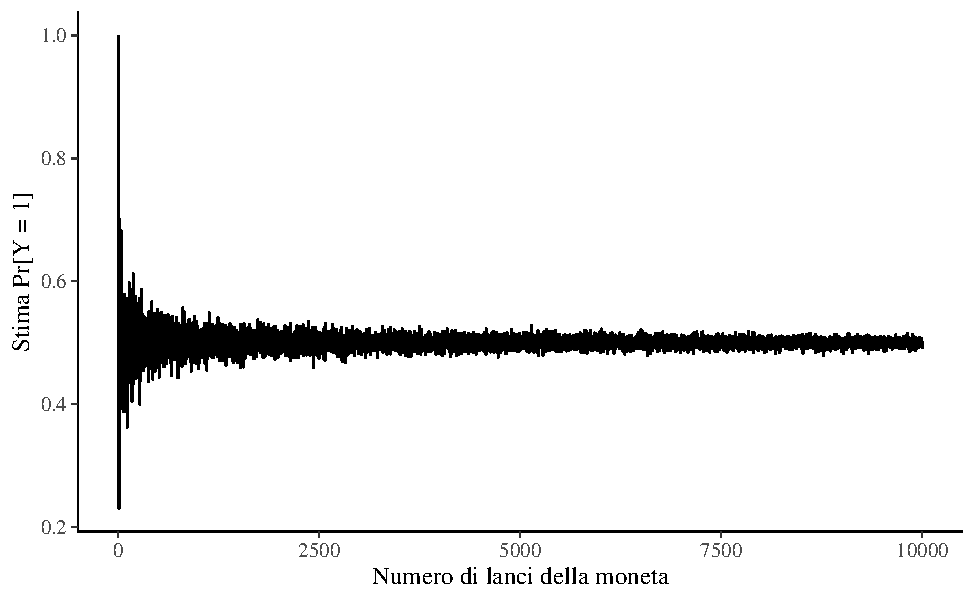
\includegraphics{ds4psy_files/figure-latex/legge-grandi-n-1-1} 

}

\caption{Stima della probabilità di successo in funzione del numero di lanci di una moneta.}\label{fig:legge-grandi-n-1}
\end{figure}

Dato che il grafico \ref{fig:legge-grandi-n-1} espresso su una scala lineare non rivela chiaramente l'andamento della simulazione, possiamo usare un grafico che impone una scala logaritmica sull'asse delle ascisse (\(x\)). Su scala logaritmica, i valori tra 1 e 10 vengono tracciati all'incirca con la stessa ampiezza che si osseerva per valori tra 50 e 700, eccetera.

\begin{Shaded}
\begin{Highlighting}[]
\NormalTok{d }\SpecialCharTok{\%\textgreater{}\%} 
  \FunctionTok{ggplot}\NormalTok{(}
    \FunctionTok{aes}\NormalTok{(}\AttributeTok{x =}\NormalTok{ n, }\AttributeTok{y =}\NormalTok{ estimate)}
\NormalTok{  ) }\SpecialCharTok{+}
  \FunctionTok{geom\_line}\NormalTok{() }\SpecialCharTok{+}
  \FunctionTok{scale\_x\_log10}\NormalTok{(}
    \AttributeTok{breaks =} \FunctionTok{c}\NormalTok{(}\DecValTok{1}\NormalTok{, }\DecValTok{3}\NormalTok{, }\DecValTok{10}\NormalTok{, }\DecValTok{50}\NormalTok{, }\DecValTok{200}\NormalTok{, }
               \DecValTok{700}\NormalTok{, }\DecValTok{2500}\NormalTok{, }\DecValTok{10000}\NormalTok{)}
\NormalTok{  ) }\SpecialCharTok{+}
  \FunctionTok{theme}\NormalTok{(}\AttributeTok{legend.title =} \FunctionTok{element\_blank}\NormalTok{()) }\SpecialCharTok{+}
  \FunctionTok{labs}\NormalTok{(}
    \AttributeTok{x =} \StringTok{"Numero di lanci della moneta"}\NormalTok{, }
    \AttributeTok{y =} \StringTok{"Stima Pr[Y = 1]"}
\NormalTok{)}
\end{Highlighting}
\end{Shaded}

\begin{figure}[h]

{\centering 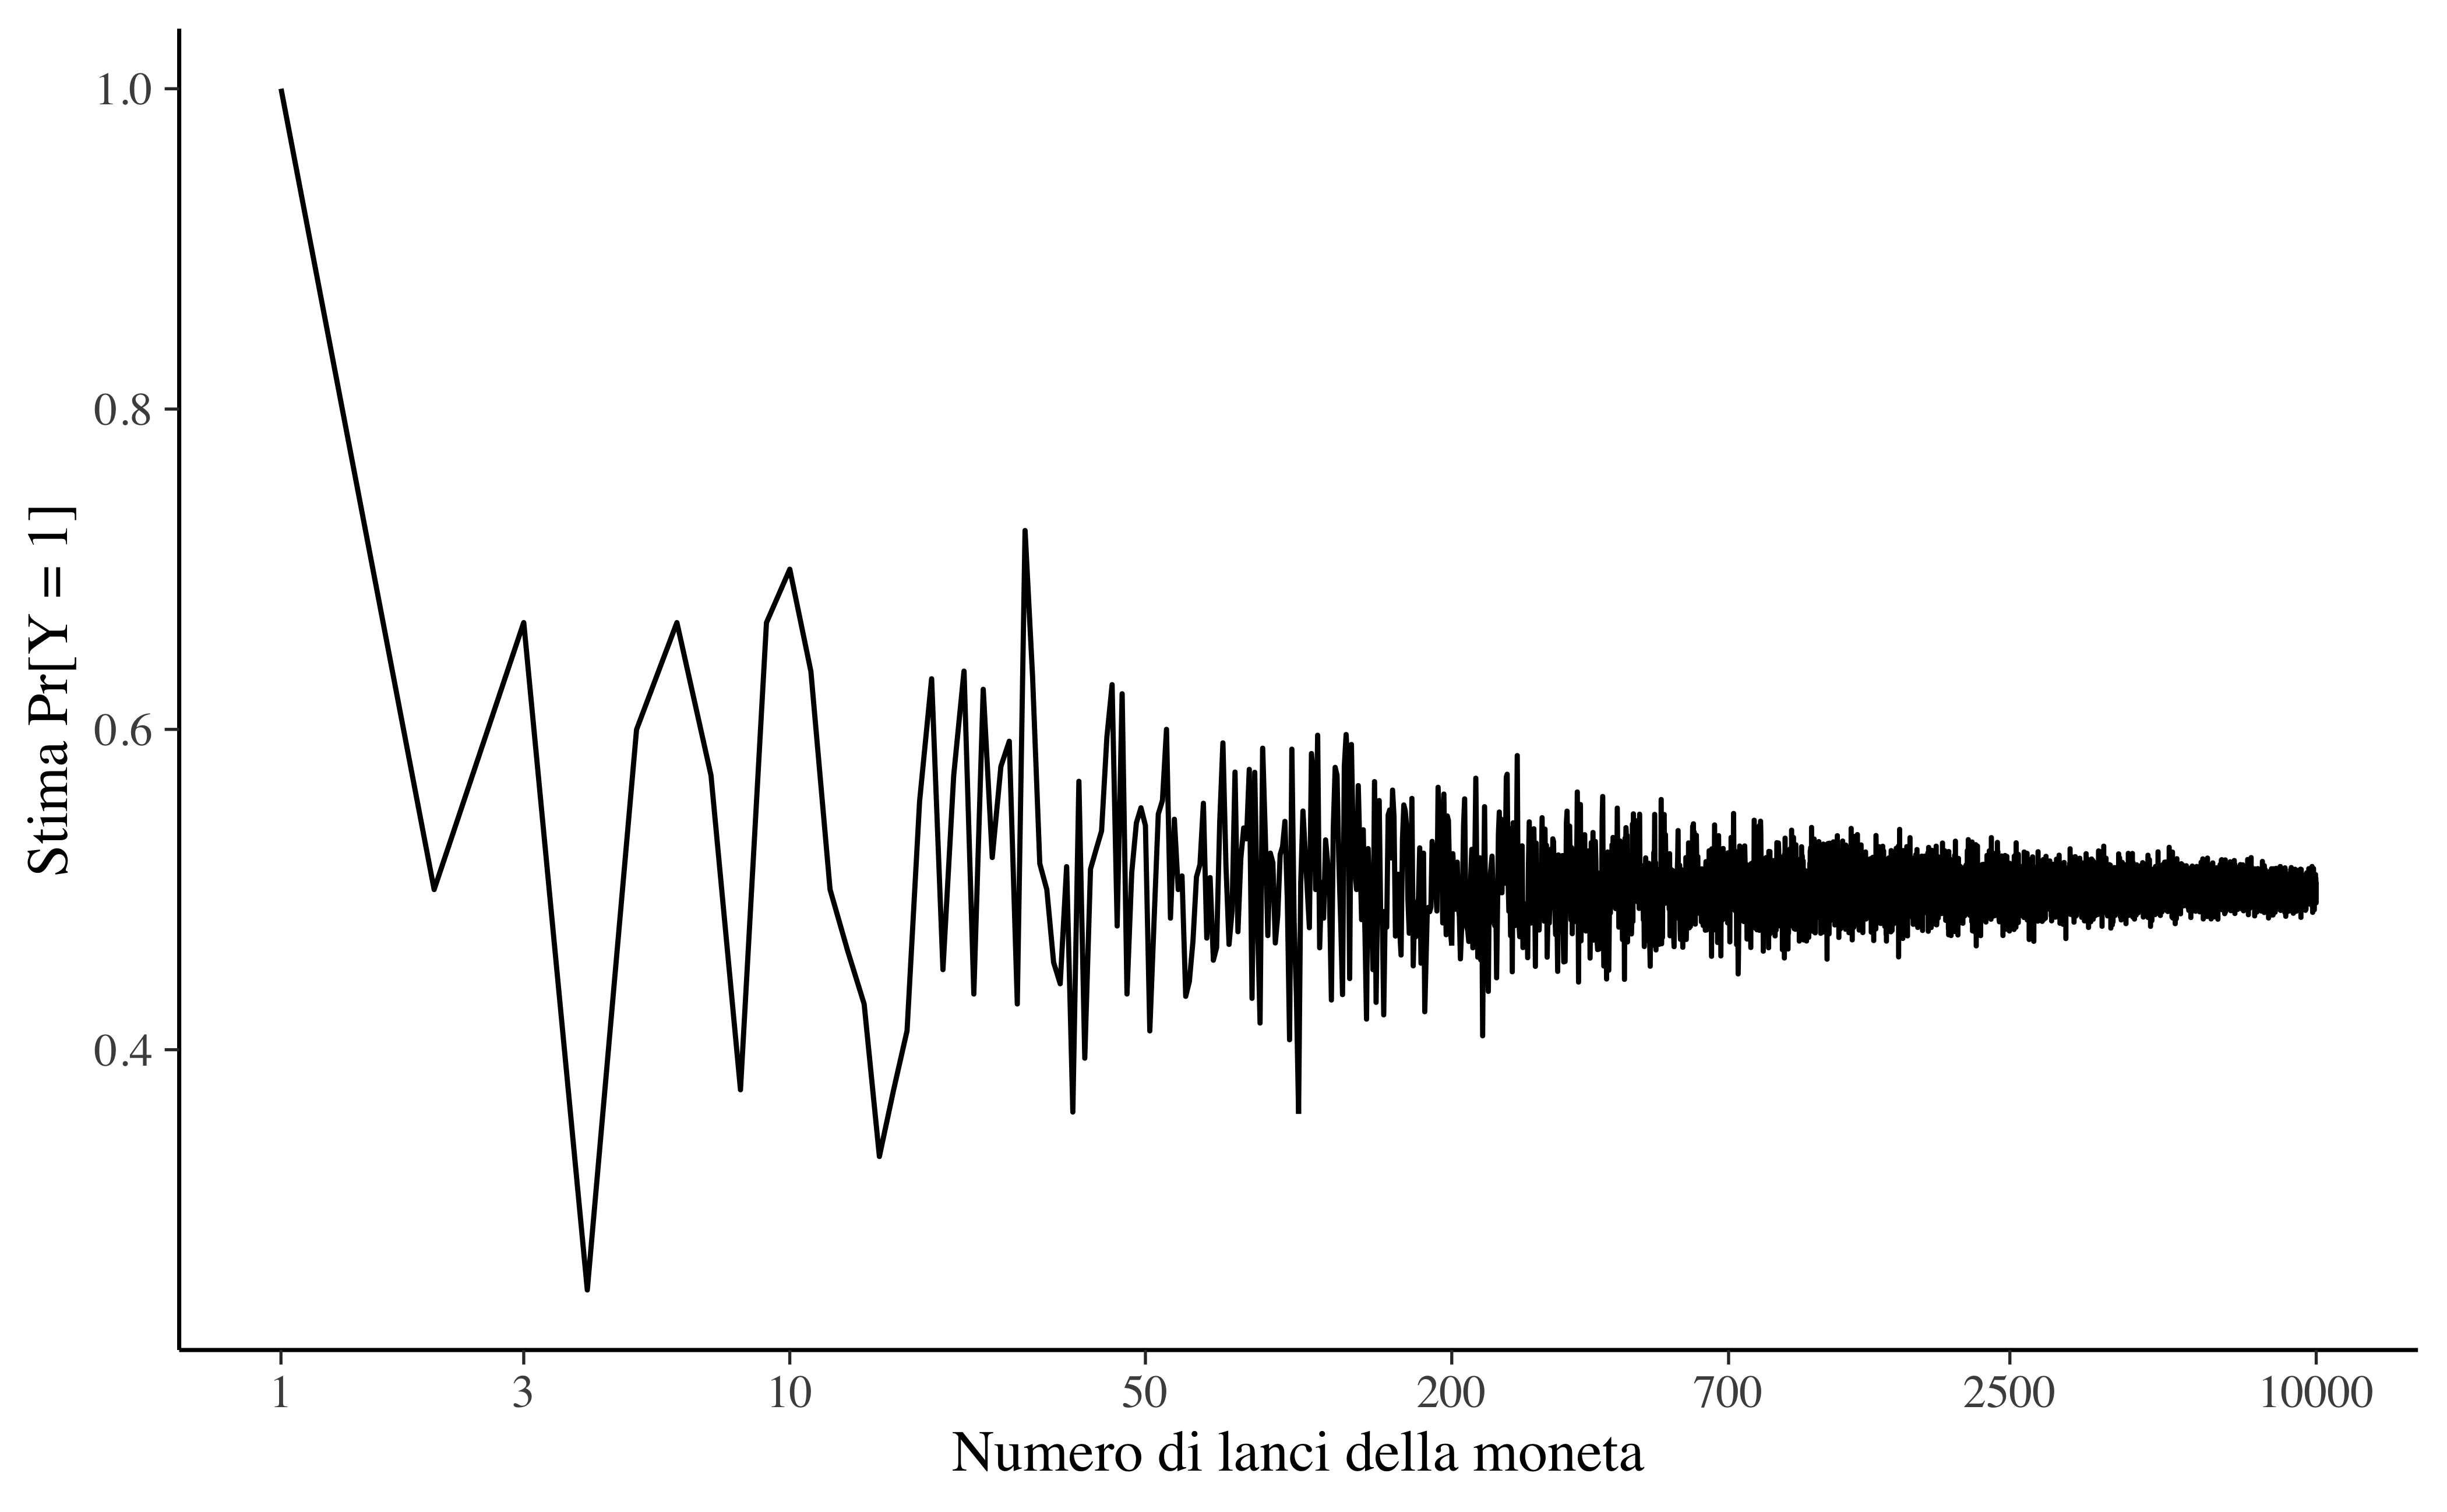
\includegraphics{ds4psy_files/figure-latex/legge-grandi-n-2-1} 

}

\caption{Stima della probabilità di successo in funzione del numero di lanci di una moneta -- scala logaritmica.}\label{fig:legge-grandi-n-2}
\end{figure}

La \emph{legge dei grandi numeri} ci dice che, all'aumentare del numero di ripetizioni dell'esperimento casuale, la media dei risultati ottenuti tenderà ad avvicinarsi al valore atteso, man mano che verranno eseguite più prove. Nel caso presente, la figura \ref{fig:legge-grandi-n-2} mostra appunto che, all'aumentare del numero \emph{M} di lanci della moneta, la stima di \(Pr[Y = 1]\) tende a convergere al vero valore di 0.5.

\hypertarget{variabili-casuali-multiple}{%
\section{Variabili casuali multiple}\label{variabili-casuali-multiple}}

Le variabili casuali non esistono isolatamente. Abbiamo iniziato con una singola variabile casuale \emph{Y} che rappresenta il risultato di un singolo, specifico lancio di una moneta equlibrata. Ma supponiamo ora di lanciare la moneta tre volte. Ciò suggerisce che i risultati di ciascuno dei tre lanci possono essere rappresentati da una diversa variabile casuale, ad esepio, \(Y_1 , Y_2 , Y_3\). Possiamo assumere che ogni lancio sia indipendente, ovvero che non dipenda dal risultato degli altri lanci. Ognuna di queste variabili \(Y_n\) per \(n \in 1:3\) ha \(Pr[Y_n =1]=0.5\) e \(Pr[Y_n =0]=0.5\).

È possibile combinare più variabili casuali usando le operazioni aritmetiche. Se \(Y_1 , Y_2, Y_3\) sono variabili casuali che rappresentano tre lanci di una moneta equilibrata (o un lancio di tre monete equilibrate), possiamo definire la somma di tali variabili casuali come

\[
Z = Y_1 + Y_2 + Y_3.
\]

Possiamo simulare i valori assunti dalla variabile casuale \emph{Z} simulando i valori di \(Y_1, Y_2, Y_3\) per poi sommarli.

\begin{Shaded}
\begin{Highlighting}[]
\NormalTok{y1 }\OtherTok{\textless{}{-}} \FunctionTok{rbinom}\NormalTok{(}\DecValTok{1}\NormalTok{, }\DecValTok{1}\NormalTok{, }\FloatTok{0.5}\NormalTok{)}
\NormalTok{y2 }\OtherTok{\textless{}{-}} \FunctionTok{rbinom}\NormalTok{(}\DecValTok{1}\NormalTok{, }\DecValTok{1}\NormalTok{, }\FloatTok{0.5}\NormalTok{)}
\NormalTok{y3 }\OtherTok{\textless{}{-}} \FunctionTok{rbinom}\NormalTok{(}\DecValTok{1}\NormalTok{, }\DecValTok{1}\NormalTok{, }\FloatTok{0.5}\NormalTok{)}
\FunctionTok{c}\NormalTok{(y1, y2, y3)}
\CommentTok{\#\textgreater{} [1] 1 0 1}
\NormalTok{z }\OtherTok{\textless{}{-}} \FunctionTok{sum}\NormalTok{(}\FunctionTok{c}\NormalTok{(y1, y2, y3))}
\FunctionTok{cat}\NormalTok{(}\StringTok{"z ="}\NormalTok{, z, }\StringTok{"}\SpecialCharTok{\textbackslash{}n}\StringTok{"}\NormalTok{)}
\CommentTok{\#\textgreater{} z = 2}
\end{Highlighting}
\end{Shaded}

ovvero,

\begin{Shaded}
\begin{Highlighting}[]
\NormalTok{y }\OtherTok{\textless{}{-}} \FunctionTok{rep}\NormalTok{(}\ConstantTok{NA}\NormalTok{, }\DecValTok{3}\NormalTok{)}
\ControlFlowTok{for}\NormalTok{ (i }\ControlFlowTok{in} \DecValTok{1}\SpecialCharTok{:}\DecValTok{3}\NormalTok{) \{}
\NormalTok{  y[i] }\OtherTok{\textless{}{-}} \FunctionTok{rbinom}\NormalTok{(}\DecValTok{1}\NormalTok{, }\DecValTok{1}\NormalTok{, }\FloatTok{0.5}\NormalTok{)}
\NormalTok{\}}
\NormalTok{y}
\CommentTok{\#\textgreater{} [1] 0 1 1}
\NormalTok{z }\OtherTok{\textless{}{-}} \FunctionTok{sum}\NormalTok{(y)}
\FunctionTok{cat}\NormalTok{(}\StringTok{"z ="}\NormalTok{, z, }\StringTok{"}\SpecialCharTok{\textbackslash{}n}\StringTok{"}\NormalTok{)}
\CommentTok{\#\textgreater{} z = 2}
\end{Highlighting}
\end{Shaded}

oppure, ancora più semplicemente:

\begin{Shaded}
\begin{Highlighting}[]
\NormalTok{y }\OtherTok{\textless{}{-}} \FunctionTok{rbinom}\NormalTok{(}\DecValTok{3}\NormalTok{, }\DecValTok{1}\NormalTok{, }\FloatTok{0.5}\NormalTok{)}
\NormalTok{y}
\CommentTok{\#\textgreater{} [1] 1 0 1}
\NormalTok{z }\OtherTok{\textless{}{-}} \FunctionTok{sum}\NormalTok{(y)}
\FunctionTok{cat}\NormalTok{(}\StringTok{"z ="}\NormalTok{, z, }\StringTok{"}\SpecialCharTok{\textbackslash{}n}\StringTok{"}\NormalTok{)}
\CommentTok{\#\textgreater{} z = 2}
\end{Highlighting}
\end{Shaded}

Possiamo ripetere questa simulazione \(M = 1e5\) volte:

\begin{Shaded}
\begin{Highlighting}[]
\NormalTok{M }\OtherTok{\textless{}{-}} \FloatTok{1e5}
\NormalTok{z }\OtherTok{\textless{}{-}} \FunctionTok{rep}\NormalTok{(}\ConstantTok{NA}\NormalTok{, M)}
\ControlFlowTok{for}\NormalTok{(i }\ControlFlowTok{in} \DecValTok{1}\SpecialCharTok{:}\NormalTok{M) \{}
\NormalTok{  y }\OtherTok{\textless{}{-}} \FunctionTok{rbinom}\NormalTok{(}\DecValTok{3}\NormalTok{, }\DecValTok{1}\NormalTok{, }\FloatTok{0.5}\NormalTok{)}
\NormalTok{  z[i] }\OtherTok{\textless{}{-}} \FunctionTok{sum}\NormalTok{(y)}
\NormalTok{\}}
\end{Highlighting}
\end{Shaded}

e calcolare una stima della probabilità che la variabile casuale \(Z\) assuma i valori 0, 1, 2, 3:

\begin{Shaded}
\begin{Highlighting}[]
\FunctionTok{table}\NormalTok{(z) }\SpecialCharTok{/}\NormalTok{ M}
\CommentTok{\#\textgreater{} z}
\CommentTok{\#\textgreater{}      0      1      2      3 }
\CommentTok{\#\textgreater{} 0.1258 0.3750 0.3748 0.1244}
\end{Highlighting}
\end{Shaded}

Nel caso di 4 monete equilibrate, avremo:

\begin{Shaded}
\begin{Highlighting}[]
\NormalTok{M }\OtherTok{\textless{}{-}} \FloatTok{1e5}
\NormalTok{z }\OtherTok{\textless{}{-}} \FunctionTok{rep}\NormalTok{(}\ConstantTok{NA}\NormalTok{, M)}
\ControlFlowTok{for}\NormalTok{(i }\ControlFlowTok{in} \DecValTok{1}\SpecialCharTok{:}\NormalTok{M) \{}
\NormalTok{  y }\OtherTok{\textless{}{-}} \FunctionTok{rbinom}\NormalTok{(}\DecValTok{4}\NormalTok{, }\DecValTok{1}\NormalTok{, }\FloatTok{0.5}\NormalTok{)}
\NormalTok{  z[i] }\OtherTok{\textless{}{-}} \FunctionTok{sum}\NormalTok{(y)}
\NormalTok{\}}
\FunctionTok{table}\NormalTok{(z) }\SpecialCharTok{/}\NormalTok{ M}
\CommentTok{\#\textgreater{} z}
\CommentTok{\#\textgreater{}       0       1       2       3       4 }
\CommentTok{\#\textgreater{} 0.06340 0.24917 0.37360 0.25022 0.06361}
\end{Highlighting}
\end{Shaded}

Una variabile casuale le cui modalità possono essere costituite solo da numeri interi è detta \emph{variabile casuale discreta}:

\[
\mathbb{Z} = \dots, -2, -1, 0, 1, 2, \dots
\]

\hypertarget{sec:fun-mass-prob}{%
\section{Funzione di massa di probabilità}\label{sec:fun-mass-prob}}

È conveniente avere una funzione che associa ogni possibile valore di una variabile casuale alla sua probabilità. In generale, ciò è possibile se e solo se la variabile casuale è discreta, così com'è stata definita nel Paragrafo precedente.

Ad esempio, se consideriamo \(Z = Y_1 + \dots + Y_4\) come il numero di risultati ``testa'' in 4 lanci della moneta, allora possiamo definire la seguente funzione:

\[
\begin{array}{rclll}
p_Z(0) & = & 1/16 & & \mathrm{TTTT}
\\
p_Z(1) & = & 4/16 & & \mathrm{HTTT, THTT, TTHT, TTTH}
\\
p_Z(2) & = & 6/16 & & \mathrm{HHTT, HTHT, HTTH, THHT, THTH, TTTH}
\\
p_Z(3) & = & 4/16 & & \mathrm{HHHT, HHTH, HTHH, THHH}
\\
p_Z(4) & = & 1/16 & & \mathrm{HHHH}
\end{array}
\]

Il lancio di quattro monete può produrre sedici possibili risultati. Dato che i lanci sono indipendenti e le monete sono equilibrate, ogni possibile risultato è ugualmente probabile. Nella tabella in alto, le sequenze dei risultati possibili del lancio delle 4 monete sono riportate nella colonna più a destra. Le probabilità si ottengono dividendo il numero di sequenze che producono lo stesso numero di eventi testa per il numero dei risultati possibili.

La funzione \(p_Z\) è stata costruita per mappare un valore \(u\) per \(Z\) alla probabilità dell'evento \(Z = u\). Convenzionalmente, queste probabilità sono scritte come

\[
p_Z(z) = \mbox{Pr}[Z = z].
\]

La parte a destra dell'uguale si può leggere come: ``la probabilità che la variabile casuale \(Z\) assuma il valore \(z\)''.

Una funzione definita come sopra è detta \emph{funzione di massa di probabilità} della variabile casuale \(Z\). Ad ogni variabile casuale discreta è associata un'unica funzione di massa di probabilità.

Una rappresentazione grafica della stima della funzione di massa di probabilità per l'esperimento casuale del lancio di quattro monete equilibrate è fornita nella figura \ref{fig:barplot-mdf-4coins}.

\begin{Shaded}
\begin{Highlighting}[]
\FunctionTok{set.seed}\NormalTok{(}\DecValTok{1234}\NormalTok{)}
\NormalTok{M }\OtherTok{\textless{}{-}} \FloatTok{1e5}
\NormalTok{nflips }\OtherTok{\textless{}{-}} \DecValTok{4}
\NormalTok{u }\OtherTok{\textless{}{-}} \FunctionTok{rbinom}\NormalTok{(M, nflips, }\FloatTok{0.5}\NormalTok{)}
\NormalTok{x }\OtherTok{\textless{}{-}} \DecValTok{0}\SpecialCharTok{:}\NormalTok{nflips}
\NormalTok{y }\OtherTok{\textless{}{-}} \FunctionTok{rep}\NormalTok{(}\ConstantTok{NA}\NormalTok{, nflips }\SpecialCharTok{+} \DecValTok{1}\NormalTok{)}
\ControlFlowTok{for}\NormalTok{ (n }\ControlFlowTok{in} \DecValTok{0}\SpecialCharTok{:}\NormalTok{nflips) \{}
\NormalTok{  y[n }\SpecialCharTok{+} \DecValTok{1}\NormalTok{] }\OtherTok{\textless{}{-}} \FunctionTok{sum}\NormalTok{(u }\SpecialCharTok{==}\NormalTok{ n) }\SpecialCharTok{/}\NormalTok{ M}
\NormalTok{\}}
\NormalTok{bar\_plot }\OtherTok{\textless{}{-}}
  \FunctionTok{data.frame}\NormalTok{(}\AttributeTok{Z =}\NormalTok{ x, }\AttributeTok{count =}\NormalTok{ y) }\SpecialCharTok{\%\textgreater{}\%}
  \FunctionTok{ggplot}\NormalTok{(}
    \FunctionTok{aes}\NormalTok{(}\AttributeTok{x =}\NormalTok{ Z, }\AttributeTok{y =}\NormalTok{ count)}
\NormalTok{  ) }\SpecialCharTok{+}
  \FunctionTok{geom\_bar}\NormalTok{(}\AttributeTok{stat =} \StringTok{"identity"}\NormalTok{) }\SpecialCharTok{+}
  \FunctionTok{scale\_x\_continuous}\NormalTok{(}
    \AttributeTok{breaks =} \DecValTok{0}\SpecialCharTok{:}\DecValTok{4}\NormalTok{,}
    \AttributeTok{labels =} \FunctionTok{c}\NormalTok{(}\DecValTok{0}\NormalTok{, }\DecValTok{1}\NormalTok{, }\DecValTok{2}\NormalTok{, }\DecValTok{3}\NormalTok{, }\DecValTok{4}\NormalTok{)}
\NormalTok{  ) }\SpecialCharTok{+}
  \FunctionTok{labs}\NormalTok{(}
    \AttributeTok{y =} \StringTok{"Probabilità stimata Pr[Z = z]"}
\NormalTok{  )}
\NormalTok{bar\_plot}
\end{Highlighting}
\end{Shaded}

\begin{figure}[h]

{\centering 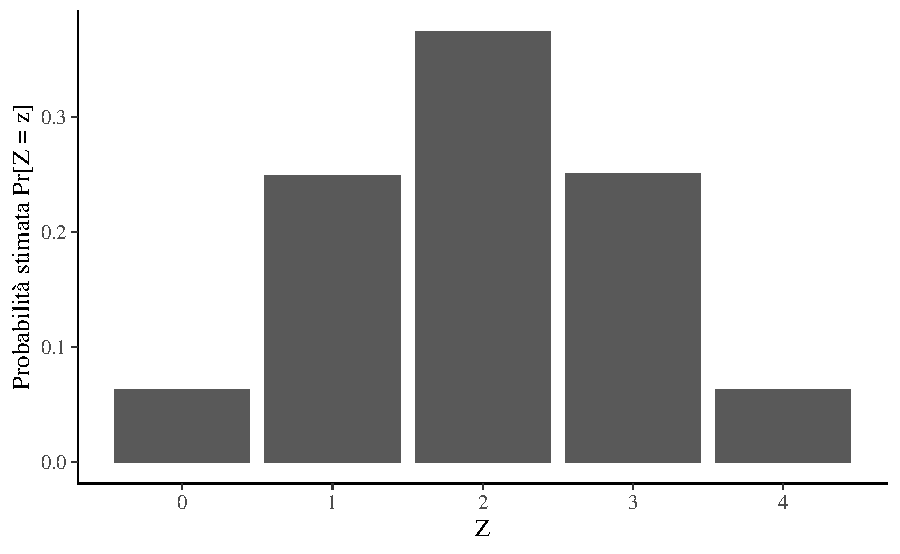
\includegraphics{ds4psy_files/figure-latex/barplot-mdf-4coins-1} 

}

\caption{Grafico di $M = 100\,000$ simulazioni della funzione di massa di probabilità di una variabile casuale definita come il numero di teste in quattro lanci di una moneta equilibrata.}\label{fig:barplot-mdf-4coins}
\end{figure}

Se \(A\) è un sottoinsieme della variabile casuale \(Z\), allora denotiamo con \(P_{z}(A)\) la probabilità assegnata ad \(A\) dalla distribuzione \(P_{z}\). Mediante una distribuzione di probabilità \(P_{z}\) è dunque possibile determinare la probabilità di ciascun sottoinsieme \(A \subset Z\) come

\[
P_{z}(A) = \sum_{z \in A} P_{z}(Z).
\]

\begin{example}
Nel caso dell'esempio discusso nella Sezione \ref{sec:fun-mass-prob}, la probabilità che la variabile casuale \(Z\) sia un numero dispari è

\[
Pr(\text{Z è un numero dispari}) = P_{z}(Z = 1) + P_{z}(Z = 3) = \frac{4}{16} + \frac{4}{16} = \frac{1}{2}.
\]
\end{example}

\hypertarget{commenti-e-considerazioni-finali}{%
\section*{Commenti e considerazioni finali}\label{commenti-e-considerazioni-finali}}


In questo capitolo abbiamo visto come si costruisce lo spazio campionario di un esperimento casuale, quali sono le proprietà di base della probabilità e come si assegnano le probabilità agli eventi definiti sopra uno spazio campionario discreto. Abbiamo anche introdotto le nozioni di ``variabile casuale'', ovvero di una variabile che prende i suoi valori casualmente. E abbiamo descritto il modo di specificare la probabilità con cui sono presi i differenti valori, ovvero la funzione di distribuzione probabilistica \(F(X) = Pr(X < x)\), e la funzione di massa di probabilità. Le procedure di analisi dei dati psicologici che discuteremo in seguito faranno un grande uso di questi concetti e della notazione qui introdotta.

\hypertarget{chapter-prob-cond}{%
\chapter{Probabilità condizionata}\label{chapter-prob-cond}}

Il fondamento della statistica bayesiana è il teorema di Bayes e il fondamento del teorema di Bayes è la probabilità condizionata. In questo Capitolo, inizieremo a presentare la probabilità condizionata. Nel Capitolo successivo, partendo dalla definizione di probabilità condizionata, deriveremo il teorema di Bayes.

\hypertarget{sec:bayes-cancer}{%
\section{Probabilità condizionata su altri eventi}\label{sec:bayes-cancer}}

L'attribuzione di una probabilità ad un evento è sempre condizionata dalle conoscenze che abbiamo a disposizione. Per un determinato stato di conoscenze, attribuiamo ad un dato evento una certa probabilità di verificarsi; ma se il nostro stato di conoscenze cambia, allora cambierà anche la probabilità che attribuiremo all'evento in questione. Infatti, si può pensare che tutte le probabilità siano probabilità condizionate, anche se l'evento condizionante non è sempre esplicitamente menzionato. Consideriamo il seguente problema.

\begin{exercise}

Supponiamo che lo screening per la diagnosi precoce del tumore mammario si avvalga di test che sono accurati al 90\%, nel senso che il 90\% delle donne con cancro e il 90\% delle donne senza cancro saranno classificate correttamente. Supponiamo che l'1\% delle donne sottoposte allo screening abbia effettivamente il cancro al seno. Ci chiediamo: qual è la probabilità che una donna scelta casualmente abbia una mammografia positiva e, se ce l'ha, qual è la probabilità che abbia davvero il cancro?

Per risolvere questo problema, supponiamo che il test in questione venga somministrato ad un grande campione di donne, diciamo a 1000 donne. Di queste 1000 donne, 10 (ovvero, l'1\%) hanno il cancro al seno. Per queste 10 donne, il test darà un risultato positivo in 9 casi (ovvero, nel 90\% dei casi). Per le rimanenti 990 donne che non hanno il cancro al seno, il test darà un risultato positivo in 99 casi (se la probabilità di un vero positivo è del 90\%, la probabilità di un falso positivo è del 10\%). Questa situazione è rappresentata nella figura \ref{fig:mammografia}.

Combinando i due risultati precedenti, vediamo che il test dà un risultato positivo per 9 donne che hanno effettivamente il cancro al seno e per 99 donne che non ce l'hanno, per un totale di 108 risultati positivi. Dunque, la probabilità di ottenere un risultato positivo al test è \(\frac{108}{1000}\) = 11\%. Ma delle 108 donne che hanno ottenuto un risultato positivo al test, solo 9 hanno il cancro al seno. Dunque, la probabilità di avere il cancro, dato un risultato positivo al test, è pari a \(\frac{9}{108}\) = 8\%.

\begin{figure}[h]

{\centering 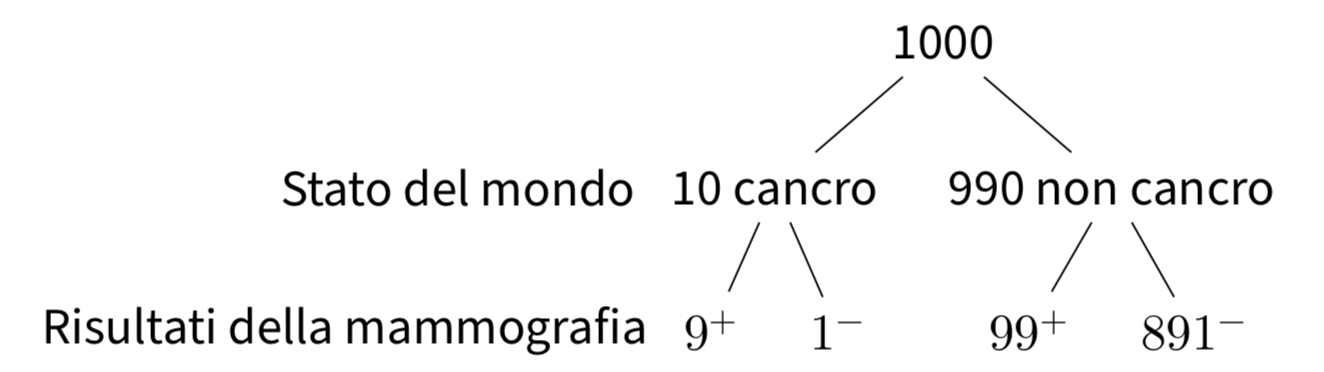
\includegraphics[width=0.67\linewidth]{images/mammografia} 

}

\caption{Rappresentazione ad albero che riporta le frequenze attese dei risultati di una mammografia in un campione di 1,000 donne.}\label{fig:mammografia}
\end{figure}

\end{exercise}

Nell'esercizio precedente, la probabilità dell'evento ``ottenere un risultato positivo al test'' è una probabilità non condizionata, mentre la probabilità dell'evento ``avere il cancro al seno, dato che il test ha prodotto un risultato positivo'' è una probabilità condizionata. In termini generali, la probabilità condizionata \(P(A \mid B)\) rappresenta la probabilità che si verifichi l'evento \(A\) sapendo che si è verificato l'evento \(B\) (oppure: la probabilità di \(A\) in una prova valida solo se si verifica anche \(B\)). Ciò ci conduce alla seguente definizione.

\begin{definition}
Dato un qualsiasi evento \(A\), si chiama \emph{probabilità condizionata} di \(A\) dato \(B\) il numero

\begin{equation}
P(A \mid B) = \frac{P(A \cap B)}{P(B)}, \quad \text{con}\, P(B) > 0,
\label{eq:probcond}
\end{equation}

dove \(P(A\cap B)\) è la probabilità congiunta dei due eventi, ovvero la probabilità che si verifichino entrambi.
\end{definition}

Nella \eqref{eq:probcond} possiamo distinguere tra la \(P(A\cap B)\), probabilità congiunta, \(P(A \cap B\), probabilità condizionata, e \(P(B)\), probabilità marginale.

Dalla definizione di probabilità condizionata è possibile esprimere la probabilità congiunta come prodotto di due probabilità, una condizionata e una marginale (\emph{regola moltiplicativa}, o \emph{della catena}). Per esempio se conosciamo la probabilità marginale \(P(B)\) e la probabilità condizionata \(P(A \mid B)\) otteniamo \begin{equation}
P(A \cap B) = P(B)P(A \mid B),
\label{eq:probcondinv}
\end{equation}

mentre se conosciamo la probabilità marginale \(P(A)\) e la probabilità condizionata \(P(B \mid A)\) otteniamo

\[
P(A \cap B) = P(A)P(B \mid A).
\]

\begin{exercise}
Da un mazzo di 52 carte (13 carte per ciascuno dei 4 semi) ne viene estratta una in modo casuale. Qual è la probabilità che esca una figura di cuori? Sapendo che la carta estratta ha il seme di cuori, qual è la probabilità che il valore numerico della carta sia 7, 8 o 9?

Ci sono 13 carte di cuori, dunque la risposta alla prima domanda è 1/4. Per rispondere alla seconda domanda consideriamo solo le 13 carte di cuori; la probabilità cercata è dunque 3/13.
\end{exercise}

\hypertarget{la-fallacia-del-condizionale-trasposto}{%
\subsection{La fallacia del condizionale trasposto}\label{la-fallacia-del-condizionale-trasposto}}

Un errore comune che si commette è quello di credere che \(P(A \mid B)\) sia uguale a \(P(B \mid A)\). Tale fallacia ha particolare risalto in ambito forense tanto che è conosciuta con il nome di ``fallacia del procuratore''. In essa, una piccola probabilità dell'evidenza, data l'innocenza, viene erroneamente interpretata come la probabilità dell'innocenza, data l'evidenza.

Consideriamo il caso di un esame del DNA. Un esperto forense potrebbe affermare, ad esempio, che ``se l'imputato è innocente, c'è solo una possibilità su un miliardo che vi sia una corrispondenza tra il suo DNA e il DNA trovato sulla scena del crimine''. Ma talvolta questa probabilità è erroneamente interpretata come avesse il seguente significato: ``date le prove del DNA, c'è solo una possibilità su un miliardo che l'imputato sia innocente''.

Le considerazioni precedenti risultano più chiare se facciamo nuovamente riferimento all'esercizio sul tumore mammario descritto sopra. In tale esercizio abbiamo visto come la probabilità di cancro dato un risultato positivo al test sia uguale a 0.08. Tale probabilità è molto diversa dalla probabilità di un risultato positivo al test data la presenza del cancro. Infatti, questa seconda probabilità è uguale a 0.90 ed è descritta nel problema come una delle caratteristiche del test in questione.

\hypertarget{legge-delle-probabilituxe0-composte}{%
\section{Legge delle probabilità composte}\label{legge-delle-probabilituxe0-composte}}

Il teorema delle probabilità composte deriva dal concetto di probabilità condizionata per cui la probabilità che si verifichino due eventi \(A_i\) e \(A_j\) è pari alla probabilità di uno dei due eventi moltiplicato con la probabilità dell'altro evento condizionato al verificarsi del primo.

L'equazione \eqref{eq:probcondinv} si estende al caso di \(n\) eventi \(A_1, \dots, A_n\) nella forma seguente:

\begin{equation}
\begin{split}
P(A_1 \cap A_2 \cap \dots\cap A_n) = {}& P(A_1)P(A_2 \mid A_1)P(A_3 \mid A_1 \cap A_2) \dots\\
 & P(A_n \mid A_1 \cap A_2 \cap \dots \cap A_{n-1})
\end{split}
\label{eq:probcomposte}
\end{equation}

la quale esprime in forma generale la legge delle probabilità composte.

\begin{exercise}
Da un'urna contenente 6 palline bianche e 4 nere si estrae una pallina per volta, senza reintrodurla nell'urna. Indichiamo con \(B_i\) l'evento: ``esce una pallina bianca alla \(i\)-esima estrazione'' e con \(N_i\) l'estrazione di una pallina nera. L'evento: ``escono due palline bianche nelle prime due estrazioni'' è rappresentato dalla intersezione \(\{B_1 \cap B_2\}\) e la sua probabilità vale, per la~\eqref{eq:probcondinv}

\[
P(B_1 \cap B_2) = P(B_1)P(B_2 \mid B_1).
\]

\(P(B_1)\) vale 6/10, perché nella prima estrazione \(\Omega\) è costituito da 10 elementi: 6 palline bianche e 4 nere. La probabilità condizionata \(P(B_2 \mid B_1)\) vale 5/9, perché nella seconda estrazione, se è verificato l'evento \(B_1\), lo spazio campionario consiste di 5 palline bianche e 4 nere. Si ricava pertanto:

\[
P(B_1 \cap B_2) = \frac{6}{10} \cdot \frac{5}{9} = \frac{1}{3}.
\]

In modo analogo si ha che

\[
P(N_1 \cap N_2) = P(N_1)P(N_2 \mid N_1) = \frac{4}{10} \cdot \frac{3}{9} = \frac{4}{30}.
\]

Se l'esperimento consiste nell'estrazione successiva di 3 palline, la probabilità che queste siano tutte bianche vale, per la \eqref{eq:probcomposte}:

\[
P(B_1 \cap B_2 \cap B_3)=P(B_1)P(B_2 \mid B_1)P(B_3 \mid B_1 \cap B_2),
\]

dove la probabilità \(P(B_3 \mid B_1 \cap B_2)\) si calcola supponendo che si sia verificato l'evento condizionante \(\{B_1 \cap B_2\}\). Lo spazio campionario per questa probabilità condizionata è costituito da 4 palline bianche e 4 nere, per cui \(P(B_3 \mid B_1 \cap B_2) = 1/2\) e quindi:

\[
P (B_1 \cap B_2 \cap B_3) = \frac{6}{10}\cdot\frac{5}{9} \cdot\frac{4}{8}  = \frac{1}{6}.
\]

La probabilità dell'estrazione di tre palline nere è invece:

\[
\begin{aligned}
P(N_1 \cap N_2 \cap N_3) &= P(N_1)P(N_2 \mid N_1)P(N_3 \mid N_1 \cap N_2)\notag\\ 
&= \frac{4}{10} \cdot \frac{3}{9} \cdot \frac{2}{8} = \frac{1}{30}.\notag
\end{aligned}
\]
\end{exercise}

\hypertarget{lindipendendenza-stocastica}{%
\section{L'indipendendenza stocastica}\label{lindipendendenza-stocastica}}

Un concetto molto importante per le applicazioni statistiche della probabilità è quello dell'indipendenza stocastica. La definizione \eqref{eq:probcond} esprime il concetto intuitivo di indipendenza di un evento da un altro, nel senso che il verificarsi di \(A\) non influisce sulla probabilità del verificarsi di \(B\), ovvero non la condiziona. Infatti, per la definizione \eqref{eq:probcond} di probabilità condizionata, si ha che, se \(A\) e \(B\) sono due eventi indipendenti, risulta:

\[
P(A \mid B) = \frac{P(A)P(B)}{P(B)} = P(A).\notag
\]

Possiamo dunque dire che due eventi \(A\) e \(B\) sono indipendenti se

\[
\begin{split}
P(A \mid B) &= P(A), \\
P(B \mid A) &= P(B).
\end{split}
\]

Si noti inoltre che, se due eventi con probabilità non nulla sono statisticamente indipendenti, la legge delle probabilità totali espressa dalla \eqref{eq:probunione} \begin{equation}
P(A \cup B) = P(A) + P(B) - P(A \cap B)
\label{eq:probunione}
\end{equation}

si modifica nella relazione seguente:

\begin{equation}
P(A \cup B) = P(A) + P(B) - P(A)P(B).
\end{equation}

\begin{exercise}
Nel lancio di due dadi non truccati, si considerino gli eventi: \emph{A} = \{esce un 1 o un 2 nel primo lancio\} e \emph{B} = \{il punteggio totale è 8\}. Gli eventi \emph{A} e \emph{B} sono indipendenti?

Rappresentiamo qui sotto lo spazio campionario dell'esperimento casuale.

\begin{figure}[h]

{\centering 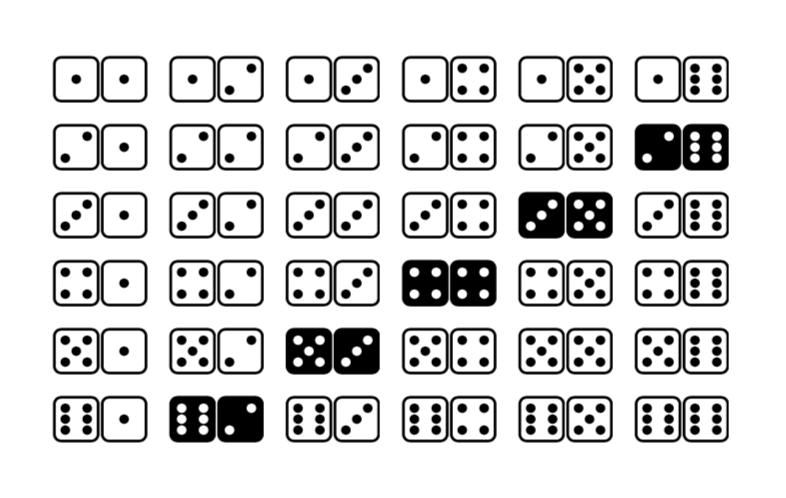
\includegraphics[width=0.7\linewidth]{images/sampling-space-dice} 

}

\caption{Rappresentazione dello spazio campionario dei risultati dell'esperimento casuale corrispondente al lancio di due dadi bilanciati. Sono evidenziati gli eventi elementari che costituiscono l'evento A: esce un 1 o un 2 nel primo lancio.}\label{fig:sampling-space-dice}
\end{figure}

Gli eventi \emph{A} e \emph{B} non sono statisticamente indipendenti. Infatti, le loro probabilità valgono \emph{P}(A) = 12/36 e \emph{P}(B) = 5/36 e la probabilità della loro intersezione è

\[
P(A \cap B) = 1/36 = 3/108 \neq P(A)P(B) = 5/108.
\]
\end{exercise}

\begin{remark}
Il concetto di indipendenza è del tutto differente da quello di incompatibilità. Si noti infatti che due eventi \emph{A} e \emph{B} incompatibili (per i quali si ha \(A \cap B = \emptyset\)) sono statisticamente dipendenti, poiché il verificarsi dell'uno esclude il verificarsi dell'altro: \(P(A \cap B)=0 \neq P(A)P(B)\).
\end{remark}

\hypertarget{commenti-e-considerazioni-finali-1}{%
\section*{Commenti e considerazioni finali}\label{commenti-e-considerazioni-finali-1}}


La probabilità condizionata è importante perché ci fornisce uno strumento per precisare il concetto di indipendenza statistica. Una delle domande più importanti delle analisi statistiche è infatti quella che si chiede se due variabili sono associate tra loro oppure no. In questo Capitolo abbiamo discusso il concetto di indipendenza (come contrapposto al concetto di associazione -- si veda il Capitolo \ref{chapter-descript}). In seguito vedremo come sia possibile fare inferenza sull'associazione tra variabili.

\hypertarget{chapter-teo-bayes}{%
\chapter{Il teorema di Bayes}\label{chapter-teo-bayes}}

Il teorema di Bayes deriva da due teoremi fondamentali delle probabilità: il \emph{teorema della probabilità composta}, ovvero \(\ {\mbox{P}}(A\cap B)={\mbox{P}}(B){\mbox{P}}(A \mid B)={\mbox{P}}(A){\mbox{P}}(B \mid A)\), e il \emph{teorema della probabilità assoluta} (detto anche \emph{teorema delle partizioni}), ovvero \({\mbox{P}}(B)=\sum _{{i=1}}^{n}{\mbox{P}}(A_{i}\cap B)=\sum _{{i=1}}^{n}{\mbox{P}}(A_{i}){\mbox{P}}(B \mid A_{i})\). Iniziamo con il teorema della probabilità assoluta.

\hypertarget{il-teorema-della-probabilituxe0-assoluta}{%
\section{Il teorema della probabilità assoluta}\label{il-teorema-della-probabilituxe0-assoluta}}

Il teorema della probabilità assoluta verrà qui presentato considerando una partizione dello spazio campionario in tre sottoinsiemi, ma è facile estendere tale discussione al caso di una partizione in un qualunque numero di sottoinsiemi.

\begin{theorem}
Sia \(\{F_1, F_2, F_3\}\) una partizione dello spazio campionario \(\Omega\). Se \(E\) è un qualunque altro evento, \(E \subset \Omega\), con \(p(E) > 0\), allora:

\begin{equation}
P(E) = P(E \cap F_1) + P(E \cap F_2) + P(E \cap F_3) \notag
\label{eq:prob-total-1a}
\end{equation}

ovvero

\begin{equation}
P(E) = P(E \mid F_1) P(F_1) + P (E \mid F_2) P(F_2) + P(E \mid F_3) P(F_3).
\label{eq:prob-total-1b}
\end{equation}
\end{theorem}

Il teorema della probabilità assoluta afferma che, se l'evento \(E\) è costituito da tutti gli eventi elementari in \(E \cap F_1\), \(E \cap F_2\) e \(E \cap F_3\), allora la probabilità \(P(E)\) è data dalla somma delle probabilità di questi tre eventi (figura \ref{fig:tikz-prob-tot}). La \citet{ref}(eq:prob-total-1b) costituisce il denominatore del teorema di Bayes,

\begin{figure}[h]

{\centering 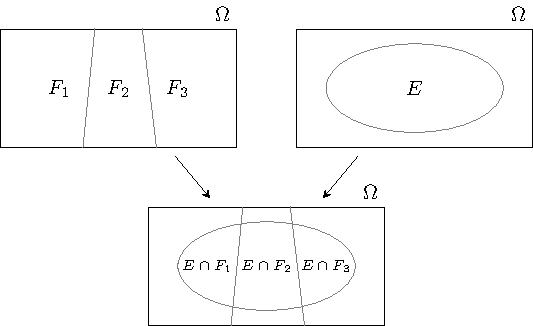
\includegraphics{ds4psy_files/figure-latex/tikz-prob-tot-1} 

}

\caption{Partizione dello spazio campionario $\Omega$.}\label{fig:tikz-prob-tot}
\end{figure}

\begin{exercise}
Si considerino tre urne, ciascuna delle quali contiene 100 palline:

\begin{itemize}
\tightlist
\item
  Urna 1: 75 palline rosse e 25 palline blu,
\item
  Urna 2: 60 palline rosse e 40 palline blu,
\item
  Urna 3: 45 palline rosse e 55 palline blu.
\end{itemize}

\noindent Una pallina viene estratta a caso da un'urna anch'essa scelta a caso. Qual è la probabilità che la pallina estratta sia di colore rosso?

Sia \(R\) l'evento ``la pallina estratta è rossa'' e sia \(U_i\) l'evento che corrisponde alla scelta dell'\(i\)-esima urna. Sappiamo che

\[
P(R \mid U_1) = 0.75, \quad P(R \mid U_2) = 0.60, \quad P(R \mid U_3) = 0.45.
\]

Gli eventi \(U_1\), \(U_2\) e \(U_3\) costituiscono una partizione dello spazio campionario in quanto \(U_1\), \(U_2\) e \(U_3\) sono eventi mutualmente esclusivi ed esaustivi, \(P(U_1 \cup U_2 \cup U_3) = 1.0\). In base al teorema della probabilità assoluta, la probabilità di estrarre una pallina rossa è dunque

\[
\begin{split}
P(R) &= P(R \mid U_1)P(U_1)+P(R \mid U_2)P(U_2)+P(R \mid U_3)P(U_3) \\
&= 0.75 \cdot \frac{1}{3}+0.60 \cdot \frac{1}{3}+0.45 \cdot \frac{1}{3} \\
&=0.60.
\end{split}
\] (Un altro esercizio sulla probabilità assoluta è fornito in Appendice \ref{appendix:exrc-abs-prob}.)
\end{exercise}

\eqref{eq:binom}

\hypertarget{il-teorema-di-bayes}{%
\section{Il teorema di Bayes}\label{il-teorema-di-bayes}}

Introduciamo ora il teorema di Bayes considerando un caso specifico per poi esaminarlo nella sua forma più generale. Sia \(\{F_1, F_2\}\) una partizione dello spazio campionario \(\Omega\). Consideriamo un terzo evento \(E \subset \Omega\) con probabilità non nulla di cui si conoscono le probabilità condizionate rispetto ad \(F_1\) e a \(F_2\), ovvero \(P(E \mid F_1)\) e \(P(E \mid F_2)\). È chiaro per le ipotesi fatte che se si verifica \(E\) deve anche essersi verificato almeno uno degli eventi \(F_1\) e \(F_2\). Supponendo che si sia verificato l'evento \(E\), ci chiediamo: qual è la probabilità che si sia verificato \(F_1\) piuttosto che \(F_2\)?

\begin{figure}[h]

{\centering 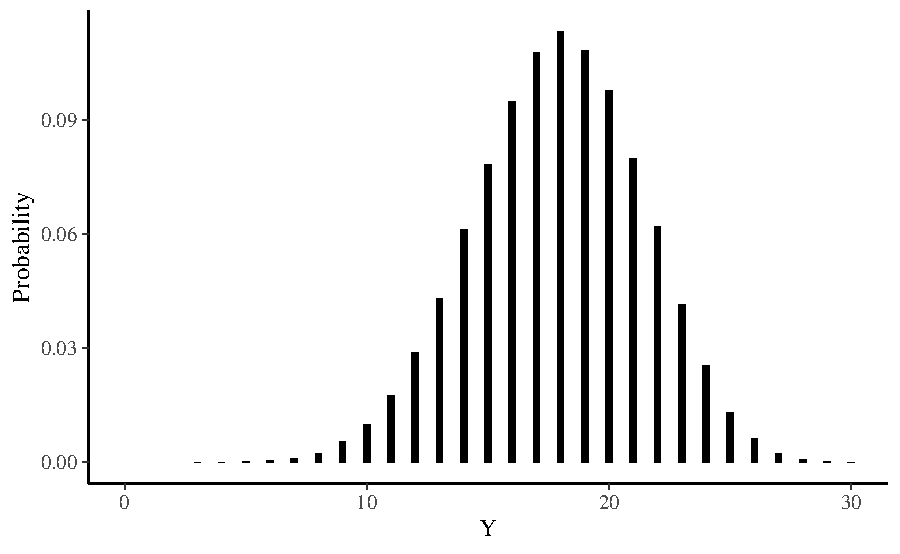
\includegraphics[width=0.45\linewidth]{ds4psy_files/figure-latex/unnamed-chunk-17-1} 

}

\end{figure}

Per rispondere alla domanda precedente scriviamo:

\[
\begin{split}
P(F_1 \mid E) &= \frac{P(E \cap F_1)}{P(E)}\notag\\
              &= \frac{P(E \mid F_1)P(F_1)}{P(E)}.
\end{split}
\]

Sapendo che \(E = (E \cap F_1) \cup (E \cap F_2)\) e che \(F_1\) e \(F_2\) sono eventi disgiunti, ovvero \(F_1 \cap F_2 = \emptyset\), ne segue che possiamo calcolare \(P(E)\) utilizzando il teorema della probabilità assoluta:

\[
\begin{split}
P(E) &= P(E \cap F_1) + P(E \cap F_2)\notag\\
     &= P(E \mid F_1)P(F_1) + P(E \mid F_2)P(F_2).
\end{split}
\]

\noindent Sostituendo il risultato precedente nella formula della probabilità condizionata \(P(F_1 \mid E)\) otteniamo:

\begin{equation}
P(F_1 \mid E) = \frac{P(E \mid F_1)P(F_1)}{P(E \mid F_1)P(F_1) + P(E \mid F_2)P(F_2)}.
\label{eq:bayes1}
\end{equation}

\noindent La \eqref{eq:bayes1} si generalizza facilmente al caso di più di due eventi disgiunti, come indicato di seguito.

\begin{theorem}
Sia \(E\) un evento contenuto in \(F_1 \cup \dots \cup F_k\), dove gli eventi \(F_j, j=1, \dots, k\) sono a due a due incompatibili e necessari. Allora per ognuno dei suddetti eventi \(F_j\) vale la seguente formula:

\begin{equation}
P(F_j \mid E) = \frac{P(E \mid F_j)P(F_j)}{\sum_{j=1}^{k}P(F_j)P(E \mid F_j)}.
\label{eq:bayes2}
\end{equation}
\end{theorem}

\noindent La \eqref{eq:bayes2} prende il nome di \emph{teorema di Bayes} e mostra che la conoscenza del verificarsi dell'evento \(E\) modifica la probabilità che avevamo attribuito all'evento \(F_j\). Nella \eqref{eq:bayes2} la probabilità condizionata \(P(F_j \mid E)\) prende il nome di probabilità \emph{a posteriori} dell'evento \(F_j\): il termine ``a posteriori'' sta a significare ``dopo che è noto che si è verificato l'evento \(E\)''.

Nel capitolo \ref{chapter-intro-bayes-inference} estenderemo questa discussione mostrando come la \eqref{eq:bayes2} può essere formulata in un modo ancora più generale, ovvero in modo tale da sostituire le funzioni di densità di probabilità alle probabilità di eventi.

\begin{remark}
Qual è la pronuncia di ``Bayesian''? Per saperlo possiamo seguire \href{https://bayes-rules.github.io/posts/fun/}{questo link}.
\end{remark}

\begin{exercise}
Un lettore attento si sarà reso conto che, in precedenza, abbiamo già applicato il teorema di Bayes, quando abbiamo risolto l'esercizio riportato nella Sezione \ref{sec:bayes-cancer}. Svolgiamo ora nuovamente lo stesso esercizio applicando questa volta la \eqref{eq:bayes2}. Per semplicità, riscriviamo la formula del teorema di Bayes nel modo seguente:

\begin{align}
P(M \mid +) &= \frac{P(+ \mid M) P(M)}{P(+ \mid M) P(M) + P(+ \mid M^\complement) P(M^\complement)}\notag\\ 
&= \frac{0.9 \cdot 10/1000}{0.9 \cdot 10/1000 + 99 / 990 \cdot 990 / 1000} \notag\\
&= \frac{9}{108}.
\end{align}

Viene così replicato il risultato precedente. Un esercizio simile è proposto in Appendice \ref{appendix:bayes-updating}.
\end{exercise}

\hypertarget{commenti-e-considerazioni-finali-2}{%
\section*{Commenti e considerazioni finali}\label{commenti-e-considerazioni-finali-2}}


Il teorema di Bayes rende esplicito il motivo per cui la probabilità non può essere pensata come uno stato oggettivo, quanto piuttosto come un'inferenza soggettiva e condizionata. Il denominatore del membro di destra della \eqref{eq:bayes2} è un semplice fattore di normalizzazione. Nel numeratore compaiono invece due quantità: \(P(F_j\)) e \(P(E \mid F_j)\). La probabilità \(P(F_j\)) è la probabilità \emph{probabilità a priori} (\emph{prior}) dell'evento \(F_j\) e rappresenta l'informazione che l'agente bayesiano possiede a proposito dell'evento \(F_j\). Diremo che \(P(F_j)\) codifica il grado di fiducia che l'agente ripone in \(F_j\) prima di avere osservato i dati. Nell'interpretazione bayesiana, \(P(F_j)\) rappresenta un giudizio personale dell'agente e non esistono criteri esterni che possano determinare se tale giudizio sia coretto o meno. La probabilità condizionata \(P(E \mid F_j)\) rappresenta invece la verosimiglianza di \(F_j\) e ci dice quant'è plausibile che si verifichi l'evento \(E\) condizionatemente al fatto che si sia verificato \(F_j\). Il teorema di Bayes descrive la regola che l'agente deve seguire per aggiornare il suo grado di fiducia in \(F_j\) alla luce di un ulteriore evento \(E\). La \(P(F_j \mid E)\) è chiamata probabilità a posteriori dato che rappresenta la nuova probabilità che l'agente assegna ad \(F_j\) affinché rimanga consistente con le nuove informazioni fornitegli da \(E\).

La probabilità a posteriori dipende sia da \(E\), sia dalla conoscenza a priori dell'agente \(P(F_j)\). In questo senso è chiaro come non abbia senso parlare di una probabilità oggettiva: per il teorema di Bayes la probabilità è definita condizionatamente alla probabilità a priori, la quale a sua volta, per definizione, è un'assegnazione soggettiva. Ne segue pertanto che ogni probabilità debba essere considerata come una rappresentazione del grado di fiducia soggettiva dell'agente. Dato che ogni assegnazione probabilistica rappresenta uno stato di conoscenza e che ciascun particolare stato di conoscenza è arbitrario, un accordo tra agenti diversi non è richiesto. Tuttavia, la teoria delle probabilità ci fornisce uno strumento che, alla luce di nuove informazioni, consente l'aggiornamento dello stato di conoscenza in un modo razionale.

Il teorema di Bayes consente di modificare una credenza a priori in maniera dinamica, via via che nuove evidenze vengono raccolte, in modo tale da formulare una credenza a posteriori la quale non è mai definitiva, ma possa sempre essere aggiornata in base alle nuove evidenze disponibili. Questo processo si chiama \emph{aggiornamento bayesiano}.

\hypertarget{chapter-prob-congiunta}{%
\chapter{Probabilità congiunta}\label{chapter-prob-congiunta}}

Per descrivere la relazione tra due variabili casuali è necessario calcolare la \emph{covarianza} e la \emph{correlazione}. Il calcolo di questi due indici richiede la conoscenza della funzione di probabilità congiunta. Obiettivo di questo Capitolo è descrivere la funzione di probabilità congiunta di due variabili casuali; esamineremo in dettaglio il caso discreto.

\hypertarget{funzione-di-probabilituxe0-congiunta}{%
\section{Funzione di probabilità congiunta}\label{funzione-di-probabilituxe0-congiunta}}

Dopo aver trattato della distribuzione di probabilità di una variabile casuale, la quale associa ad ogni evento elementare dello spazio campionario uno ed un solo numero reale, è naturale estendere questo concetto al caso di due o più variabili casuali. Iniziamo a descrivere il caso discreto con un esempio. Consideriamo l'esperimento casuale corrispondente al lancio di tre monete equilibrate. Lo spazio campionario è

\[
\Omega = \{TTT, TTC, TCT, CTT, CCT, CTC, TCC, CCC\}.
\]

Dato che i tre lanci sono tra loro indipendenti, non c'è ragione di aspettarsi che uno degli otto risultati possibili dell'esperimento sia più probabile degli altri, dunque possiamo associare a ciascuno degli otto eventi elementari dello spazio campionario la stessa probabilità, ovvero 1/8.

Siano \(X \in \{0, 1, 2, 3\}\) = ``numero di realizzazioni con il risultato testa nei tre lanci'' e \(Y \in \{0, 1\}\) = ``numero di realizzazioni con il risultato testa nel primo lancio'' due variabili casuali definite sullo spazio campionario \(\Omega\). Indicando con T = `testa' e C = `croce', si ottiene la situazione riportata nella tabella \ref{tab:tre-monete-distr-cong-1}.

\begin{longtable}[]{@{}cccc@{}}
\caption{\label{tab:tre-monete-distr-cong-1} Spazio campionario dell'esperimento consistente nel lancio di tre monete equilibrate su cui sono state definite le variabili aleatorie \(X\) e \(Y\).}\tabularnewline
\toprule
\(\omega\) & \(X\) & \(Y\) & \(P(\omega)\) \\
\midrule
\endfirsthead
\toprule
\(\omega\) & \(X\) & \(Y\) & \(P(\omega)\) \\
\midrule
\endhead
\(\omega_1\) = TTT & 3 & 1 & 1/8 \\
\(\omega_2\) = TTC & 2 & 1 & 1/8 \\
\(\omega_3\) = TCT & 2 & 1 & 1/8 \\
\(\omega_4\) = CTT & 2 & 0 & 1/8 \\
\(\omega_5\) = CCT & 1 & 0 & 1/8 \\
\(\omega_6\) = CTC & 1 & 0 & 1/8 \\
\(\omega_7\) = TCC & 1 & 1 & 1/8 \\
\(\omega_8\) = CCC & 0 & 0 & 1/8 \\
\bottomrule
\end{longtable}

Ci poniamo il problema di associare un livello di probabilità ad ogni coppia \((x, y)\) definita su \(\Omega\). La coppia \((X = 0, Y = 0)\) si realizza in corrispondenza di un solo evento elementare, ovvero CCC; avrà dunque una probabilità pari a \(P(X=0, Y=0) = P(CCC) = 1/8\). Nel caso della coppia \((X = 1, Y = 0)\) ci sono due eventi elementari che danno luogo al risultato considerato, ovvero, CCT e CTC; la probabilità \(P(X=1, Y=0)\) sarà dunque data dalla probabilità dell'unione dei due eventi elementari, cioé \(P(X=1, Y=0) = P(CCT \:\cup\: CTC) = 1/8 + 1/8 = 1/4\). Sono riportati qui sotto i calcoli per tutti i possibili valori di \(X\) e \(Y\).

\begin{align}
P(X = 0, Y = 0) &= P(\omega_8 = CCC) = 1/8; \notag\\
P(X = 1, Y = 0) &= P(\omega_5 = CCT) + P(\omega_6 = CTC) = 2/8; \notag\\
P(X = 1, Y = 1) &= P(\omega_7 = TCC) = 1/8; \notag\\
P(X = 2, Y = 0) &= P(\omega_4 = CTT) = 1/8; \notag\\
P(X = 2, Y = 1) &= P(\omega_3 = TCT) + P(\omega_2 = TTC) = 2/8; \notag\\
P(X = 3, Y = 1) &= P(\omega_1 = TTT) = 1/8; \notag
\end{align}

Le probabilità così trovate sono riportate nella tabella \ref{tab:ditr-cong-biv-1} la quale descrive la distribuzione di probabilità congiunta delle variabili casuali \(X\) = ``numero di realizzazioni con il risultato testa nei tre lanci'' e \(Y\) = ``numero di realizzazioni con il risultato testa nel primo lancio'' per l'esperimento casuale consistente nel lancio di tre monete equilibrate.

\begin{longtable}[]{@{}ccc@{}}
\caption{\label{tab:ditr-cong-biv-1} Distribuzione di probabilità congiunta per i risultati dell'esperimento consistente nel lancio di tre monete equilibrate.}\tabularnewline
\toprule
\(x / y\) & 0 & 1 \\
\midrule
\endfirsthead
\toprule
\(x / y\) & 0 & 1 \\
\midrule
\endhead
0 & 1/8 & 0 \\
1 & 2/8 & 1/8 \\
2 & 1/8 & 2/8 \\
3 & 0 & 1/8 \\
\bottomrule
\end{longtable}

In generale, possiamo dire che, dato uno spazio campionario discreto \(\Omega\), è possibile associare ad ogni evento elementare \(\omega_i\) dello spazio campionario una coppia di numeri reali \((x, y)\), essendo \(x = X(\omega)\) e \(y = Y(\omega)\), il che ci conduce alla seguente definizione.

\begin{definition}
Siano \(X\) e \(Y\) due variabili casuali. La funzione che associa ad ogni coppia \((x, y)\) un livello di probabilità prende il nome di funzione di probabilità congiunta:

\[
P(x, y) = P(X = x, Y = y).
\]
\end{definition}

\noindent Il termine ``congiunta'' deriva dal fatto che questa probabilità è legata al verificarsi di una coppia di valori, il primo associato alla variabile casuale \(X\) ed il secondo alla variabile casuale \(Y\). Nel caso di due sole variabili casuali si parla di distribuzione bivariata, mentre nel caso di più variabili casuali si parla di distribuzione multivariata.

\hypertarget{proprietuxe0}{%
\subsection{Proprietà}\label{proprietuxe0}}

Una distribuzione di massa di probabilità congiunta bivariata deve soddisfare due proprietà:

\begin{enumerate}
\def\labelenumi{\arabic{enumi}.}
\item
  \(0 \leq P(x_i, y_j) \leq 1\);
\item
  la probabilità totale deve essere uguale a \(1.0\). Tale proprietà può essere espressa nel modo seguente
\end{enumerate}

\[
\sum_{i} \sum_{j} P(x_i, y_j) = 1.0.
\]

\hypertarget{eventi}{%
\subsection{Eventi}\label{eventi}}

Si noti che dalla probabilità congiunta possiamo calcolare la probabilità di qualsiasi evento definito in base alle variabili aleatorie \(X\) e \(Y\). Per capire come questo possa essere fatto, consideriamo nuovamente l'esperimento casuale discusso in precedenza.

\begin{exercise}
Per la distribuzione di massa di probabilità congiunta riportata nella tabella precedente si trovi la probabilità dell'evento \(X+Y \leq 1\).

Per trovare la probabilità richiesta dobbiamo semplicemente sommare le probabilità associate a tutte le coppie \((x,y)\) che soddisfano la condizione \(X+Y \leq 1\), ovvero

\begin{equation}
P_{XY}(X+Y \leq 1) = P_{XY}(0, 0) + P_{XY}(1, 0)= 3/8.\notag
\end{equation}
\end{exercise}

\hypertarget{regola-della-catena}{%
\subsection{Regola della catena}\label{regola-della-catena}}

Regola della catena permette il calcolo di qualsiasi membro della distribuzione congiunta di un insieme di variabili casuali utilizzando solo le probabilità condizionate.

\begin{definition}
Dati due eventi \(A\) e \(B\), la regola della catena afferma che

\[
P(A \cap B) = P(A)P(B \mid A).
\]
\end{definition}

Nel caso di 4 eventi, per esempio, la regola della catena diventa

\[
P(A_1, A_2, A_3, A_4) = P(A_1) P(A_2 \mid A_1) P(A_3 \mid A_1, A_2) P(A_4 \mid A_1, A_2, A_3).
\]

\hypertarget{sec:marg-distr-discr}{%
\subsection{Funzioni di probabilità marginali}\label{sec:marg-distr-discr}}

Nel caso di due variabili casuali discrete \(X\) e \(Y\) di cui conosciamo la distribuzione congiunta, la distribuzione marginale di \(X\) è calcolata sommando la distribuzione di probabilità congiunta sopra la variabile da ``scartare'', in questo caso la \(Y\). La funzione di massa di probabilità marginale \(P(X=x)\) è

\begin{equation}
P(X = x) = \sum_y P(X, Y = y) = \sum_y P(X \mid Y = y) P(Y = y),
\end{equation}

dove \(P(X = x,Y = y)\) è la distribuzione congiunta di \(X, Y\), mentre \(P(X = x \mid Y = y)\) è la distribuzione condizionata di \(X\) dato \(Y\). Se esaminiamo \(P(X=x)\), diciamo che la variabile \(Y\) è stata marginalizzata. Le probabilità bivariate marginali e congiunte per variabili casuali discrete sono spesso mostrate come tabelle di contingenza.

Si noti che \(P(X = x)\) e \(P(Y = y)\) sono normalizzate:

\[
\sum_x P(X=x) = 1.0, \quad \sum_y P(Y=y) = 1.0.
\]

Nel caso continuo si sostituisce l'integrazione alla somma -- si veda la Sezione \ref{sec:margin-vc-cont}.

\begin{exercise}

Per l'esperimento casuale consistente nel lancio di tre monete equilibrate, si calcolino le probabilità marginali di \(X\) e \(Y\).

Nell'ultima colonna a destra e nell'ultima riga in basso della tabella \ref{tab:ditr-cong-biv} sono riportate le distribuzioni di probabilità marginali di \(X\) e \(Y\). \(P_X\) si ottiene sommando su ciascuna riga fissata la colonna \(j\), \(P_X(X = j) = \sum_y p_{xy}(x = j, y)\). \(P_Y\) si trova sommando su ciascuna colonna fissata la riga \(i,\) \(P_Y (Y = i) = \sum_x p_{xy}(x, y = i)\).

\begin{longtable}[]{@{}cccc@{}}
\caption{\label{tab:ditr-cong-biv} Distribuzione di probabilità congiunta \(p(x,y)\) per i risultati dell'esperimento consistente nel lancio di tre monete equilibrate e probabilità marginali \(P(x)\) e \(P(y)\).}\tabularnewline
\toprule
\(x / y\) & 0 & 1 & \(P(x)\) \\
\midrule
\endfirsthead
\toprule
\(x / y\) & 0 & 1 & \(P(x)\) \\
\midrule
\endhead
0 & 1/8 & 0 & 1/8 \\
1 & 2/8 & 1/8 & 3/8 \\
2 & 1/8 & 2/8 & 3/8 \\
3 & 0 & 1/8 & 1/8 \\
\(P(y)\) & 4/8 & 4/8 & 1.0 \\
\bottomrule
\end{longtable}

\end{exercise}

\hypertarget{indipendenza-stocastica-incondizionata}{%
\section{Indipendenza stocastica incondizionata}\label{indipendenza-stocastica-incondizionata}}

In precedenza abbiamo visto come l'indipendenza stocastica di due eventi \(A\) e \(B\) si ha quando il verificarsi di uno non modifica la probabilità di verificarsi dell'altro, ovvero quando \(P(A \mid B = P(A)\) e \(P(B \mid A) = P(B)\). Queste due condizioni si possono sintetizzare con la formula \(P(A \cap B) = P(A) P(B)\).

Analogamente, quando si afferma che due variabili casuali \(X\) e \(Y\) definite sullo stesso spazio campionario \(\Omega\) sono indipendenti si afferma che conoscere qualcosa riguardo al valore di una di esse non apporta alcuna informazione circa il valore dell'altra. Formalmente, questo si verifica quando

\begin{equation}
P(X, Y)\, = P_X(x)P_Y(y).
\end{equation}

Nel caso discreto, dunque, l'indipendenza implica che la probabilità riportata in ciascuna cella della tabella di probabilità congiunta deve essere uguale al prodotto delle probabilità marginali di riga e di colonna:

\[
P(x_i, y_i)\, = P_X(x_i) P_Y(y_i).
\]

\begin{exercise}
Per la situazione rappresentata nella tabella \ref{tab:ditr-cong-biv} le variabili casuali \(X\) e \(Y\) sono indipendenti?

Nella tabella le variabili casuali \(X\) e \(Y\) non sono indipendenti: le probabilità congiunte non sono ricavabili dal prodotto delle marginali. Per esempio, nessuna delle probabilità marginali è uguale a \(0\) per cui nessuno dei valori dentro la tabella (probabilità congiunte) che risulta essere uguale a \(0\) può essere il prodotto delle probabilità marginali.
\end{exercise}

\hypertarget{indipendenza-condizionata-tra-eventi}{%
\section{Indipendenza condizionata tra eventi}\label{indipendenza-condizionata-tra-eventi}}

Sebbene l'indipendenza incondizionata sia una proprietà utile, non capita spesso di incontrare due eventi indipendenti. Una situazione più comune è quando due eventi sono indipendenti dato un terzo evento. Ad esempio, supponiamo di voler ragionare sulla possibilità che uno studente che è in possesso di un titolo di laurea triennale venga accettato al Corso di Laurea Magistrale (CdL) \(A\) o al CdL Magistrale \(B\). Nella maggior parte dei casi, questi due eventi non sono indipendenti. Se apprendiamo che lo studente è stato accettato al CdL \(A\), la nostra stima della sua probabilità che venga accettato al CdL \(B\) è ora più alta, poiché è aumentata la nostra credenza che lo studente in questione sia uno studente ``promettente''.

Ora, supponiamo che entrambi i CdL basino le loro decisioni unicamente sul voto di laurea triennale (chiamiamolo \(C\)) dello studente e supponiamo di sapere che, per lo studente in questione, \(C = 105/110\). In questo caso, apprendere che lo studente è stato ammesso al CdL \(A\) non cambia la probabilità che venga ammesso al CdL \(B\): il suo voto di laurea \(V\) fornisce tutte le informazioni rilevanti circa la possibilità che lo studente venga ammesso al CdL \(A\); sapere che è stato ammesso al CdL \(B\) non aggiunge niente a tutto ciò. Formalmente, possiamo scrivere

\begin{equation}
P(A \mid B \cap C) = P(A \mid B)
\end{equation}

Se la condizione precedente si verifica, gli eventi \(A\) e \(B\) si dicono condizionatamente indipendenti dall'evento \(C\).

Alternativamente, possiamo dire che gli eventi \(A\) e \(B\) sono condizionatamente indipendenti dall'evento \(C\) se e solo se

\begin{equation}
P(A \mid B \cap C) = P(A \mid C) P(B \mid C),
\end{equation}

oppure, maniera equivalente se

\[
P(A \mid B, C)= P(A \mid C).
\]

Poiché la probabilità di \(A\) dato \(C\) è uguale alla probabilità di \(A\) dati sia \(B\) che \(C\), questa uguaglianza esprime il fatto che \(B\) non aggiunge nulla alla nostra conoscenza della probabilità di \(A\).

Solitamente, l'indipendenza condizionata viene indicata utilizzando la notazione \((A \indep B \mid C)\).

\hypertarget{indipendenza-di-variabili-casuali}{%
\section{Indipendenza di variabili casuali}\label{indipendenza-di-variabili-casuali}}

Siano \(X, Y, Z\) tre variabili casuali. Diciamo che \(X\) è condizionatamente indipendente da \(Y\) data \(Z\) in una distribuzione \(P\) se \(P\) soddisfa \((X=x \indep Y=y \mid Z=z)\) per tutti i valori \(x \in X\), \(y \in Y\) e \(z \in Z\). Se l'insieme \(Z\) è vuoto, invece di scrivere \((X \indep Y \mid \emptyset)\), scriviamo \((X \mid Y)\) e diciamo che \(X\) e \(Y\) sono \emph{marginalmente indipendenti}.

Da ciò segue la seguente definizione alternativa di indipendenza condizionata.

\begin{definition}
La distribuzione \(P\) soddisfa \((X \indep Y \mid Z)\) se e solo se

\[
P(X, Y \mid Z) = (X \mid Z)P(Y \mid Z).
\]
\end{definition}

\hypertarget{sec:margin-vc-cont}{%
\section{Marginalizzazione di variabili casuali continue}\label{sec:margin-vc-cont}}

Nella trattazione della statistca bayesiana useremo spesso il concetto di ``marginalizzazione'' e vedremo equazioni come la seguente:

\begin{equation}
p(y) = \int_{\theta} p(y, \theta) = \int_{\theta} p(y \mid \theta) p(\theta),
\label{eq:ex-marg-cont}
\end{equation}

laddove \(y\) e \(\theta\) sono due variabili casuali continue -- nello specifico, con \(y\) denoteremo i dati e con \(\theta\) i parametri di un modello statistico. Per ora, possiamo pensare a \(y\) e \(\theta\) come a due variabili casuali qualsiasi. La \eqref{eq:ex-marg-cont} descrive la distribuzione marginale di \(y\).

Per meglio comprendere la \eqref{eq:ex-marg-cont} possiamo esaminare il corrispondente caso discreto nel quale sostituiamo semplicemente l'integrale con una somma, il che ci riporta alla situazione descritta nella Sezione \ref{sec:marg-distr-discr}. Possiamo dunque scrivere:

\begin{equation}
p(y) = \sum_{\theta} p(y, \theta) = \sum_{\theta} p(y \mid \theta) p(\theta).
\label{eq:ex-marginalization}
\end{equation}

Esaminiamo un semplice esempio numerico. Siano \(y\) e \(\theta\) due variabili discrete aventi la distribuzione di massa di probabilità congiunta riportata nella tabella \ref{tab:ex-marg}.

\begin{longtable}[]{@{}cccl@{}}
\caption{\label{tab:ex-marg} Distribuzione di probabilità congiunta \(p(y, \theta)\) per due variabili casuali discrete.}\tabularnewline
\toprule
\(y / \theta\) & 0 & 1 & \(p(y)\) \\
\midrule
\endfirsthead
\toprule
\(y / \theta\) & 0 & 1 & \(p(y)\) \\
\midrule
\endhead
0 & 0.1 & 0.2 & 0.3 \\
1 & 0.3 & 0.4 & 0.7 \\
\(p(\theta)\) & 0.4 & 0.6 & 1.0 \\
\bottomrule
\end{longtable}

Applicando la \eqref{eq:ex-marginalization}, la distribuzione marginale \(p(y) = \{0.3, 0.7\}\) può essere trovata nel modo seguente:

\[
\begin{pmatrix}
    0.1 / 0.4 \\
    0.3 / 0.4
\end{pmatrix} \cdot 0.4 +
\begin{pmatrix}
    0.2 / 0.6 \\
    0.4 / 0.6
\end{pmatrix} \cdot 0.6 =
\begin{pmatrix}
    0.3 \\
   0.7
\end{pmatrix}.
\]

È possibiile pensare al caso continuo indicato nella \eqref{eq:ex-marg-cont} come all'estensione dell'esempio presente ad un numero infinito di valori \(\theta\).

\hypertarget{commenti-e-considerazioni-finali-3}{%
\section*{Commenti e considerazioni finali}\label{commenti-e-considerazioni-finali-3}}


La funzione di probabilità congiunta tiene simultaneamente conto del comportamento di due variabili casuali \(X\) e \(Y\) e di come esse si influenzano reciprocamente. In particolare, si osserva che se le due variabili discrete \(X\) e \(Y\) non si influenzano, cioè se sono statisticamente indipendenti, allora la distribuzione di massa di probabilità congiunta si ottiene come prodotto delle funzioni di probabilità marginali di \(X\) e \(Y\): \(P_{X, Y}(x, y) = P_X(x) P_Y(y)\).

\hypertarget{chapter-intro-density-function}{%
\chapter{Funzione di densità di probabilità}\label{chapter-intro-density-function}}

Finora abbiamo considerato solo variabili casuali discrete, cioè variabili che assumono solo valori interi. Ma cosa succede se vogliamo usare variabili casuali per rappresentare lunghezze o volumi o distanze una qualsiasi delle altre proprietà continue nel mondo fisico (o psicologico)? È necessario generalizzare l'approccio usato finora.

Le variabili casuali continue assumono valori reali. L'insieme dei numeri reali è \emph{non numerabile} perché è più grande dell'insieme degli interi.\footnote{Georg Cantor dimostrò che era impossibile mappare uno a uno i reali negli interi, dimostrando così che l'insieme dei reali è non numerabile.} Le leggi della probabilità sono le stessa per le variabili casuali discrete e quelle continue. La nozione di funzione di massa di probabilità, invece, deve essere sostituita dal suo equivalente continuo, ovvero dalla funzione di densità di probabilità. Lo scopo di questo Capitolo è quello di chiarire il significato di questa nozione, usando un approccio basato sulle simulazioni.

\hypertarget{spinner-e-variabili-casuali-continue-uniformi}{%
\section{Spinner e variabili casuali continue uniformi}\label{spinner-e-variabili-casuali-continue-uniformi}}

Consideriamo il seguente esperimento casuale. Facciamo ruotare ad alta velocità uno spinner simmetrico imperniato su un goniometro e osserviamo la posizione in cui si ferma (individuata dall'angolo acuto con segno tra il suo asse e l'asse orizzontale del goniometro). Chiamiamo \(\Theta\) la variabile casuale ``pendenza dello spinner''. Nella trattazione seguente useremo i gradi e, di conseguenza, \(\Theta \in [0, 360]\).

\begin{figure}[h]

{\centering 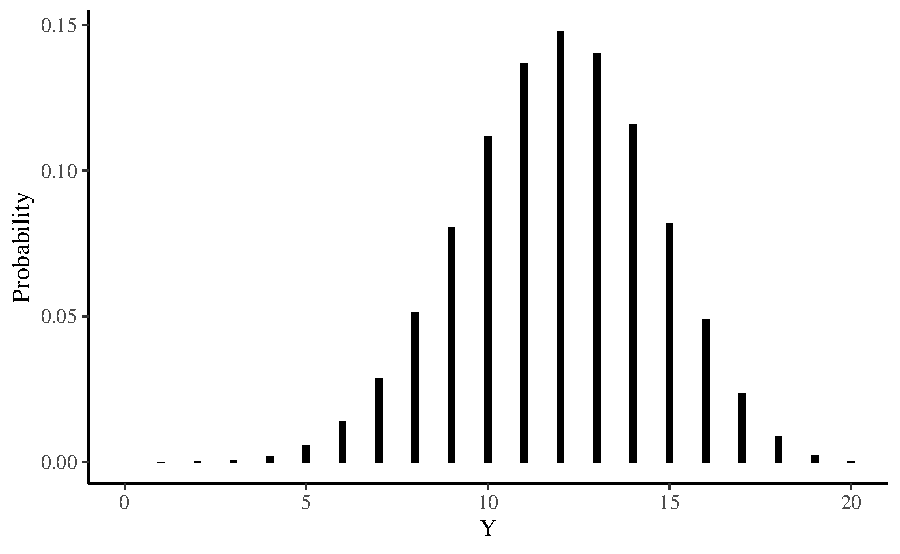
\includegraphics[width=1\linewidth]{ds4psy_files/figure-latex/unnamed-chunk-18-1} 

}

\caption{Uno spinner che riposa a 36 gradi, o il dieci percento del percorso intorno al cerchio. La pendenza dello spinner può assumere qualunque valore tra 0 e 360 gradi.}\label{fig:unnamed-chunk-18}
\end{figure}

Cosa implica per \(\Theta\) dire che lo spinner è simmetrico? Possiamo dire che, in ciascuna prova, la rotazione dello spinner produce un angolo qualunque da 0 a 360 gradi. In altri termini, un valore \(\Theta\) compreso tra 0 e 36 gradi ha la stessa probabilità di essere osservato di un valore \(\Theta\) compreso tra 200 e 236 gradi. Inoltre, poiché 36 gradi è un decimo del percorso intorno al cerchio, la probabilità di ottenere un qualsiasi intervallo di 36 gradi sarà sempre uguale al 10\%. Ovvero \(\mbox{P}[0 \leq \Theta \leq 36] \ = \ \frac{1}{10}\) e \(\mbox{P}[200 \leq \Theta \leq 236] \ = \ \frac{1}{10}\).

È importante notare che le considerazioni precedenti non si riferiscono al fatto che \(\Theta\) può assumere uno specifico valore, ma piuttosto alla probabilità di osservare \(\Theta\) in un particolare intervallo di valori. In generale, la probabilità che la pendenza \(\Theta\) dello spinner cada in intervallo è la frazione del cerchio rappresentata dall'intervallo, cioè,

\[
\mbox{P}[\theta_1 \leq \Theta \leq \theta_2] = \frac{\theta_2 - \theta_1}{360}, \qquad 0 \leq \theta_1 \leq \theta_2 \leq 360.
\]

La ragione di questo è che le variabili casuali continue non hanno una massa di probabilità. Invece, una massa di probabilità viene assegnata alla realizzazione della variabile casuale in un intervallo di valori.

\hypertarget{il-paradosso-delle-variabili-casuali-continue}{%
\subsection{Il paradosso delle variabili casuali continue}\label{il-paradosso-delle-variabili-casuali-continue}}

Nel nostro esempio, la pendenza dello spinner è esattamente 36 gradi; ma avrebbe potuto anche essere 36.0376531 gradi o qualunque altro valore in quell'intorno. Qual è la probabilità che la pendenza dello spinner sia esattamente 36? Paradossalmente, la risposta è zero:

\[
\mbox{P}[\Theta = 36] = 0.
\]

Infatti, se la probabilità di un qualunque valore fosse maggiore di zero, ogni altro possibile valore dovrebbe avere la stessa probabilità, dato che abbiamo assumiamo che tutti i valori \(\Theta\) sono egualmente probabili. Ma se poi andiamo a sommare tutte queste probabilità il totale diventerà maggiore di uno, il che non è possibile.

Nel caso delle variabili casuali continue dobbiamo dunque rinunciare a qualcosa, e quel qualcosa è l'idea che, in una distribuzione continua, ciascun valore puntuale della variabile casuale possa avere una massa di probabilità maggiore di zero. Il paradosso sorge perché una realizzazione della variabile casuale conrtinua produce sempre un qualche numero, ma ciscuno di tali numeri ha probabilità nulla.

\hypertarget{la-funzione-di-ripartizione-per-una-variabile-casuale-continua}{%
\section{La funzione di ripartizione per una variabile casuale continua}\label{la-funzione-di-ripartizione-per-una-variabile-casuale-continua}}

Supponiamo che \(\Theta \sim \mbox{uniform}(0, 360)\) sia la pendenza dello spinner. La funzione di ripartizione (ovvero, la distribuzione cumulativa) è definita esattamente come nel caso delle variabili casuali discrete:

\[
F_{\Theta}(\theta) = \mbox{P}[\Theta \leq \theta].
\]

Cioè, è la probabilità che la variabile casuale \(\Theta\) assuma un valore minore di o uguale a \(\theta\). In questo caso, poiché si presume che lo spinner sia simmetrico, la funzione di distribuzione cumulativa è

\[
F_{\Theta}(\theta) = \frac{\theta}{360}.
\]

Questa è una funzione lineare di \(\theta\), cioè \(\frac{1}{360} \times \theta\), come indicato dal grafico della figura \ref{fig:spinner-cdf}.

\begin{figure}[h]

{\centering 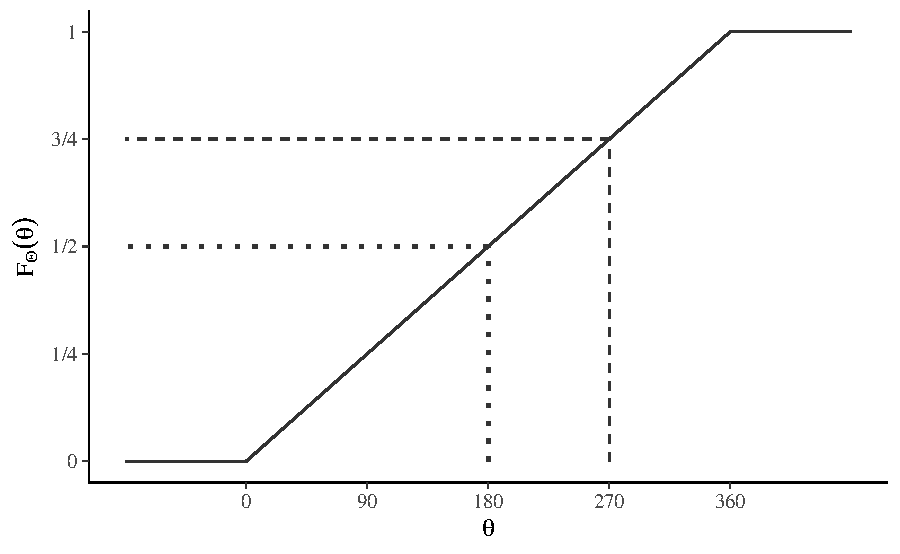
\includegraphics{ds4psy_files/figure-latex/spinner-cdf-1} 

}

\caption{Funzione di distribuzione cumulativa per l'angolo $\theta$ (in gradi) risultante da una rotazione di uno spinner simmetrico. La linea tratteggiata mostra il valore a 180 gradi, che corrisponde ad una probabilità di 0.5, e la linea tratteggiata a 270 gradi, che corrisponde ad una probabilità di 0.75.}\label{fig:spinner-cdf}
\end{figure}

Possiamo verificare questo risultato mediante simulazione. Per stimare la funzione di ripartizione, simuliamo \(M\) valori \(\theta^{(m)}\) e poi li ordiniamo in ordine crescente.

\begin{Shaded}
\begin{Highlighting}[]
\NormalTok{M }\OtherTok{\textless{}{-}} \DecValTok{1000}
\NormalTok{theta }\OtherTok{\textless{}{-}} \FunctionTok{runif}\NormalTok{(M, }\DecValTok{0}\NormalTok{, }\DecValTok{360}\NormalTok{)}
\NormalTok{theta\_asc }\OtherTok{\textless{}{-}} \FunctionTok{sort}\NormalTok{(theta)}
\NormalTok{prob }\OtherTok{\textless{}{-}}\NormalTok{ (}\DecValTok{1}\SpecialCharTok{:}\NormalTok{M) }\SpecialCharTok{/}\NormalTok{ M}
\NormalTok{unif\_cdf\_df }\OtherTok{\textless{}{-}} \FunctionTok{data.frame}\NormalTok{(}
  \AttributeTok{theta =}\NormalTok{ theta\_asc,}
  \AttributeTok{prob =}\NormalTok{ prob}
\NormalTok{)}
\NormalTok{unif\_cdf\_plot }\OtherTok{\textless{}{-}}
\NormalTok{  unif\_cdf\_df }\SpecialCharTok{\%\textgreater{}\%}
  \FunctionTok{ggplot}\NormalTok{(}\FunctionTok{aes}\NormalTok{(}\AttributeTok{x =}\NormalTok{ theta, }\AttributeTok{y =}\NormalTok{ prob)) }\SpecialCharTok{+}
  \FunctionTok{geom\_line}\NormalTok{() }\SpecialCharTok{+}
  \FunctionTok{scale\_x\_continuous}\NormalTok{(}\AttributeTok{breaks =} \FunctionTok{c}\NormalTok{(}\DecValTok{0}\NormalTok{, }\DecValTok{90}\NormalTok{, }\DecValTok{180}\NormalTok{, }\DecValTok{270}\NormalTok{, }\DecValTok{360}\NormalTok{)) }\SpecialCharTok{+}
  \FunctionTok{scale\_y\_continuous}\NormalTok{(}\AttributeTok{breaks =} \FunctionTok{c}\NormalTok{(}\DecValTok{0}\NormalTok{, }\FloatTok{0.25}\NormalTok{, }\FloatTok{0.5}\NormalTok{, }\FloatTok{0.75}\NormalTok{, }\FloatTok{1.0}\NormalTok{)) }\SpecialCharTok{+}
  \FunctionTok{xlab}\NormalTok{(}\FunctionTok{expression}\NormalTok{(theta)) }\SpecialCharTok{+}
  \FunctionTok{ylab}\NormalTok{(}\FunctionTok{expression}\NormalTok{(F[Theta](theta)))}
\NormalTok{unif\_cdf\_plot}
\end{Highlighting}
\end{Shaded}

\begin{figure}[h]

{\centering 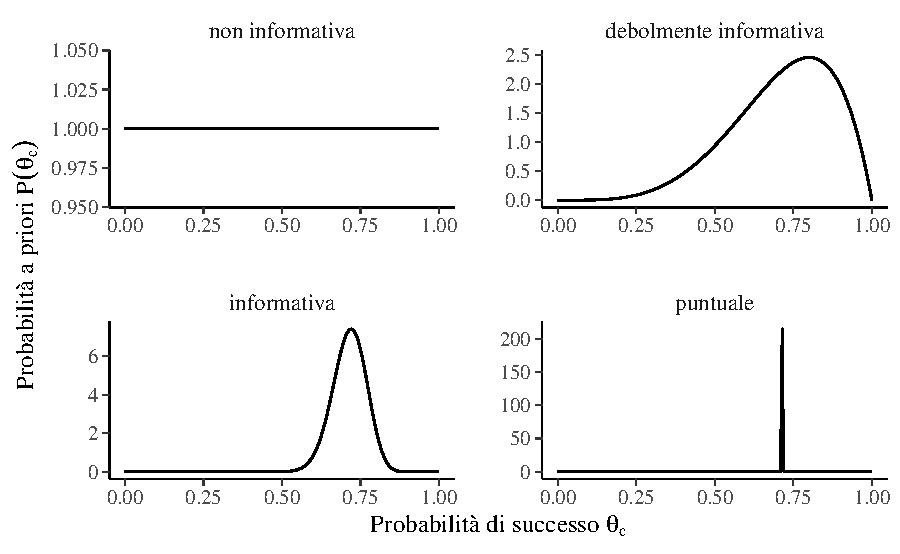
\includegraphics{ds4psy_files/figure-latex/unnamed-chunk-19-1} 

}

\caption{Grafico della funzione di ripartizione di una variabile casuale $\Theta$ che rappresenta il risultato di una rotazione di uno spinner simmetrico. Come previsto, tale funzione è una semplice funzione lineare perché la variabile sottostante $\Theta$ ha una distribuzione uniforme.}\label{fig:unnamed-chunk-19}
\end{figure}

Anche con \emph{M} = 1000, tale grafico è praticamente indistinguibile da quello prodotto per via analitica.

Come nel caso delle variabili casuali discrete, la funzione di ripartizione può essere utilizzata per calcolare le probabilità che la variabile casuale assuma valori in un intervallo. Ad esempio

\begin{align}
\mbox{P}[180 < \Theta \leq 270] &= \mbox{P}[\Theta \leq 270] \ - \ \mbox{P}[\Theta \leq 180] \notag\\
&= F_{\Theta}(270) - F_{\Theta}(180)\notag\\
&= \frac{3}{4} - \frac{1}{2} \notag\\
&= \frac{1}{4}.\noindent
\end{align}

\hypertarget{la-distribuzione-uniforme}{%
\section{La distribuzione uniforme}\label{la-distribuzione-uniforme}}

Dopo avere visto come generare numeri casuali uniformi da 0 a 360, consideriamo ora una variabile casuale che assume valori nell'intervallo da 0 a 1. Chiamiamo tale variabile casuale \(\Theta\) e assumiamo che abbia una distribuzione continua uniforme sull'intervallo {[}0, 1{]}:

\[
\Theta \sim Uniform(0, 1).
\]

Poiché le probabilità assumono valori nell'intervallo {[}0, 1{]}, possiamo pensare a \(\Theta\) come ad un valore di probabilità preso a caso in ciascuna realizzazione dell'esperimento casuale.

La distribuzione uniforme è la più semplice delle distribuzioni di densità di probabilità. Per chiarire le proprietà di tale distribuzione, iniziamo con una simulazione e generiamo 10,000 valori casuali di \(\Theta\). I primi 10 di tali valori sono stampati qui di seguito:

\begin{Shaded}
\begin{Highlighting}[]
\FunctionTok{set.seed}\NormalTok{(}\DecValTok{1234}\NormalTok{)}
\NormalTok{M }\OtherTok{\textless{}{-}} \DecValTok{10000}
\NormalTok{logit }\OtherTok{\textless{}{-}} \ControlFlowTok{function}\NormalTok{(x) }\FunctionTok{log}\NormalTok{(x }\SpecialCharTok{/}\NormalTok{ (}\DecValTok{1} \SpecialCharTok{{-}}\NormalTok{ x))}
\NormalTok{theta }\OtherTok{\textless{}{-}} \FunctionTok{runif}\NormalTok{(M)}
\NormalTok{alpha }\OtherTok{\textless{}{-}} \FunctionTok{logit}\NormalTok{(theta)}
\ControlFlowTok{for}\NormalTok{ (m }\ControlFlowTok{in} \DecValTok{1}\SpecialCharTok{:}\DecValTok{10}\NormalTok{)}
  \FunctionTok{print}\NormalTok{(alpha[m])}
\CommentTok{\#\textgreater{} [1] {-}2.053}
\CommentTok{\#\textgreater{} [1] 0.4993}
\CommentTok{\#\textgreater{} [1] 0.4443}
\CommentTok{\#\textgreater{} [1] 0.5039}
\CommentTok{\#\textgreater{} [1] 1.823}
\CommentTok{\#\textgreater{} [1] 0.5767}
\CommentTok{\#\textgreater{} [1] {-}4.647}
\CommentTok{\#\textgreater{} [1] {-}1.194}
\CommentTok{\#\textgreater{} [1] 0.6905}
\CommentTok{\#\textgreater{} [1] 0.05702}
\end{Highlighting}
\end{Shaded}

Creaiamo ora un istogramma che descrive la distribuzione delle 10,000 realizzazioni \(\Theta\) che abbiamo trovato:

\begin{Shaded}
\begin{Highlighting}[]
\NormalTok{df\_prob\_unif }\OtherTok{\textless{}{-}} \FunctionTok{data.frame}\NormalTok{(}\AttributeTok{theta =}\NormalTok{ theta)}
\NormalTok{unif\_prob\_plot }\OtherTok{\textless{}{-}}
  \FunctionTok{ggplot}\NormalTok{(df\_prob\_unif, }\FunctionTok{aes}\NormalTok{(theta)) }\SpecialCharTok{+}
  \FunctionTok{geom\_histogram}\NormalTok{(}
    \AttributeTok{binwidth =} \DecValTok{1} \SpecialCharTok{/} \DecValTok{34}\NormalTok{, }\AttributeTok{center =} \DecValTok{1} \SpecialCharTok{/} \DecValTok{68}\NormalTok{, }\AttributeTok{color =} \StringTok{"black"}\NormalTok{,}
    \AttributeTok{size =} \FloatTok{0.25}
\NormalTok{  ) }\SpecialCharTok{+}
  \FunctionTok{scale\_x\_continuous}\NormalTok{(}\AttributeTok{breaks =} \FunctionTok{c}\NormalTok{(}\DecValTok{0}\NormalTok{, }\FloatTok{0.25}\NormalTok{, }\FloatTok{0.5}\NormalTok{, }\FloatTok{0.75}\NormalTok{, }\DecValTok{1}\NormalTok{)) }\SpecialCharTok{+}
  \FunctionTok{scale\_y\_continuous}\NormalTok{(}\AttributeTok{lim =} \FunctionTok{c}\NormalTok{(}\DecValTok{0}\NormalTok{, }\DecValTok{1300}\NormalTok{), }\AttributeTok{breaks =} \FunctionTok{c}\NormalTok{(}\DecValTok{500}\NormalTok{, }\DecValTok{1000}\NormalTok{)) }\SpecialCharTok{+}
  \FunctionTok{xlab}\NormalTok{(}\FunctionTok{expression}\NormalTok{(}\FunctionTok{paste}\NormalTok{(Theta, }\StringTok{" \textasciitilde{} Uniform(0, 1)"}\NormalTok{)))}
\NormalTok{unif\_prob\_plot}
\end{Highlighting}
\end{Shaded}

\begin{figure}[h]

{\centering 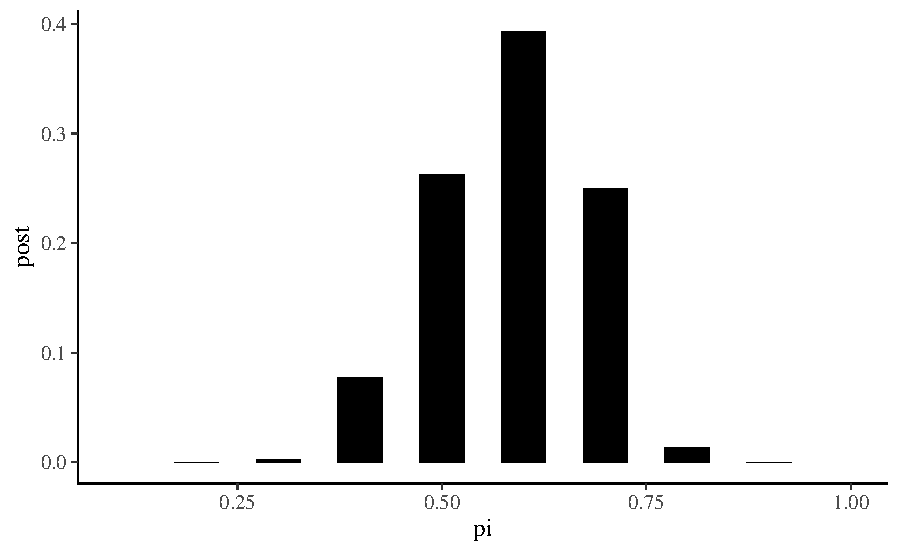
\includegraphics{ds4psy_files/figure-latex/unnamed-chunk-21-1} 

}

\caption{Istogramma di $10\,000$ realizzazioni $\Theta \sim \mbox{Uniform}(0, 1)$. }\label{fig:unnamed-chunk-21}
\end{figure}

È chiaro che, all'aumentare del numero delle realizzazioni \(\Theta\), il profilo dell'istogramma tenderà a diventare una linea retta. Ciò significa che la funzione di densità di una variabile casuale uniforme continua è una costante. Cioè, se \(\Theta \sim \mbox{Uniform} (a, b)\), allora \(p_{\Theta}(\theta) = c\), dove \(c\) è una costante.

\begin{Shaded}
\begin{Highlighting}[]
\NormalTok{uniform\_pdf\_df }\OtherTok{\textless{}{-}} \FunctionTok{data.frame}\NormalTok{(}\AttributeTok{y =} \FunctionTok{c}\NormalTok{(}\DecValTok{0}\NormalTok{, }\DecValTok{1}\NormalTok{), }\AttributeTok{p\_y =} \FunctionTok{c}\NormalTok{(}\DecValTok{1}\NormalTok{, }\DecValTok{1}\NormalTok{))}
\NormalTok{uniform\_pdf\_plot }\OtherTok{\textless{}{-}}
  \FunctionTok{ggplot}\NormalTok{(uniform\_pdf\_df, }\FunctionTok{aes}\NormalTok{(}\AttributeTok{x =}\NormalTok{ y, }\AttributeTok{y =}\NormalTok{ p\_y)) }\SpecialCharTok{+}
  \FunctionTok{geom\_line}\NormalTok{(}\AttributeTok{size =} \FloatTok{0.5}\NormalTok{, }\AttributeTok{color =} \StringTok{"\#333333"}\NormalTok{) }\SpecialCharTok{+}
  \FunctionTok{geom\_point}\NormalTok{(}\AttributeTok{size =} \FloatTok{1.5}\NormalTok{, }\AttributeTok{color =} \StringTok{"\#333333"}\NormalTok{) }\SpecialCharTok{+}
  \FunctionTok{scale\_x\_continuous}\NormalTok{(}\AttributeTok{breaks =} \FunctionTok{c}\NormalTok{(}\DecValTok{0}\NormalTok{, }\DecValTok{1}\NormalTok{), }\AttributeTok{labels =} \FunctionTok{c}\NormalTok{(}\StringTok{"a"}\NormalTok{, }\StringTok{"b"}\NormalTok{)) }\SpecialCharTok{+}
  \FunctionTok{scale\_y\_continuous}\NormalTok{(}
    \AttributeTok{lim =} \FunctionTok{c}\NormalTok{(}\DecValTok{0}\NormalTok{, }\DecValTok{1}\NormalTok{), }\AttributeTok{breaks =} \FunctionTok{c}\NormalTok{(}\DecValTok{0}\NormalTok{, }\DecValTok{1}\NormalTok{),}
    \AttributeTok{labels =} \FunctionTok{c}\NormalTok{(}\StringTok{"0"}\NormalTok{, }\StringTok{"c"}\NormalTok{)}
\NormalTok{  ) }\SpecialCharTok{+}
  \FunctionTok{xlab}\NormalTok{(}\FunctionTok{expression}\NormalTok{(theta)) }\SpecialCharTok{+}
  \FunctionTok{ylab}\NormalTok{(}\FunctionTok{expression}\NormalTok{(}\FunctionTok{paste}\NormalTok{(p[Theta], }\StringTok{"("}\NormalTok{, theta, }\StringTok{" | a, b)"}\NormalTok{))) }\SpecialCharTok{+}
  \FunctionTok{geom\_segment}\NormalTok{(}\FunctionTok{aes}\NormalTok{(}\AttributeTok{x =} \DecValTok{0}\NormalTok{, }\AttributeTok{y =} \DecValTok{0}\NormalTok{, }\AttributeTok{xend =} \DecValTok{0}\NormalTok{, }\AttributeTok{yend =} \DecValTok{1}\NormalTok{),}
    \AttributeTok{linetype =} \StringTok{"dotted"}
\NormalTok{  ) }\SpecialCharTok{+}
  \FunctionTok{geom\_segment}\NormalTok{(}\FunctionTok{aes}\NormalTok{(}\AttributeTok{x =} \DecValTok{1}\NormalTok{, }\AttributeTok{y =} \DecValTok{0}\NormalTok{, }\AttributeTok{xend =} \DecValTok{1}\NormalTok{, }\AttributeTok{yend =} \DecValTok{1}\NormalTok{),}
    \AttributeTok{linetype =} \StringTok{"dotted"}
\NormalTok{  ) }\SpecialCharTok{+}
  \FunctionTok{geom\_segment}\NormalTok{(}\FunctionTok{aes}\NormalTok{(}\AttributeTok{x =} \DecValTok{0}\NormalTok{, }\AttributeTok{y =} \DecValTok{0}\NormalTok{, }\AttributeTok{xend =} \DecValTok{1}\NormalTok{, }\AttributeTok{yend =} \DecValTok{0}\NormalTok{),}
    \AttributeTok{linetype =} \StringTok{"dotted"}
\NormalTok{  ) }\SpecialCharTok{+}
  \FunctionTok{geom\_segment}\NormalTok{(}\FunctionTok{aes}\NormalTok{(}\AttributeTok{x =} \SpecialCharTok{{-}}\FloatTok{0.25}\NormalTok{, }\AttributeTok{y =} \DecValTok{0}\NormalTok{, }\AttributeTok{xend =} \DecValTok{0}\NormalTok{, }\AttributeTok{yend =} \DecValTok{0}\NormalTok{)) }\SpecialCharTok{+}
  \FunctionTok{geom\_segment}\NormalTok{(}\FunctionTok{aes}\NormalTok{(}\AttributeTok{x =} \DecValTok{1}\NormalTok{, }\AttributeTok{y =} \DecValTok{0}\NormalTok{, }\AttributeTok{xend =} \FloatTok{1.25}\NormalTok{, }\AttributeTok{yend =} \DecValTok{0}\NormalTok{)) }\SpecialCharTok{+}
  \FunctionTok{geom\_point}\NormalTok{(}\FunctionTok{aes}\NormalTok{(}\AttributeTok{x =} \DecValTok{0}\NormalTok{, }\AttributeTok{y =} \DecValTok{0}\NormalTok{),}
    \AttributeTok{size =} \FloatTok{1.5}\NormalTok{, }\AttributeTok{shape =} \DecValTok{21}\NormalTok{,}
    \AttributeTok{fill =} \StringTok{"\#ffffe6"}
\NormalTok{  ) }\SpecialCharTok{+}
  \FunctionTok{geom\_point}\NormalTok{(}\FunctionTok{aes}\NormalTok{(}\AttributeTok{x =} \DecValTok{1}\NormalTok{, }\AttributeTok{y =} \DecValTok{0}\NormalTok{),}
    \AttributeTok{size =} \FloatTok{1.5}\NormalTok{, }\AttributeTok{shape =} \DecValTok{21}\NormalTok{,}
    \AttributeTok{fill =} \StringTok{"\#ffffe6"}
\NormalTok{  )}
\NormalTok{uniform\_pdf\_plot}
\end{Highlighting}
\end{Shaded}

\begin{center}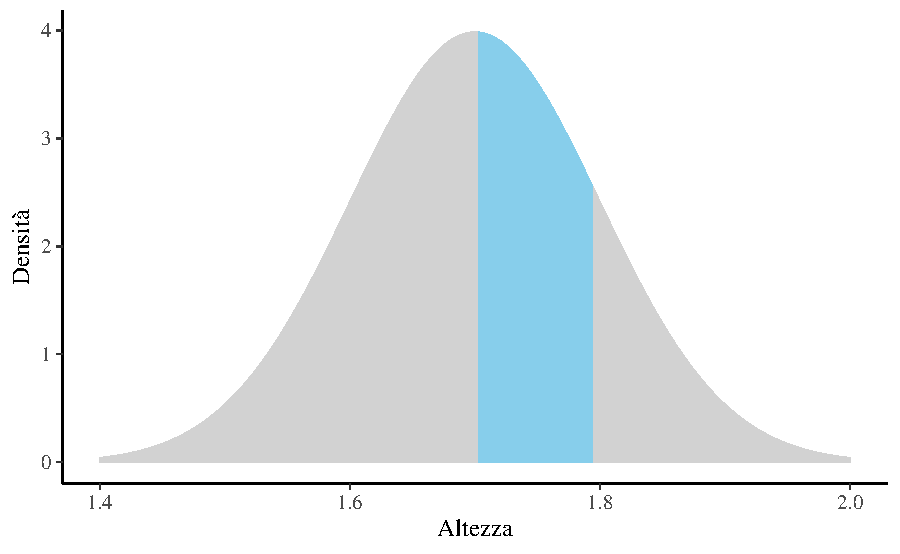
\includegraphics{ds4psy_files/figure-latex/unnamed-chunk-22-1} \end{center}

\noindent Dal grafico vediamo che l'area sottesa alla funzione di densità è \((b - a)\times c\). Dato che tale area deve essere unitaria, ovvero, \((b - a) \times c = 1\), possiamo trovare \(c\) dividendo entrambi i termini per \(b - a\),

\[
c  = \frac{\displaystyle{1}}{\displaystyle b - a}.
\]

Ovvero, se \(\Theta \sim \mbox{Uniform}(a, b)\), allora

\[
p_{\Theta}(\theta) = \mbox{Uniform}(\theta \mid a, b),
\]

laddove

\[
\mbox{Uniform}(\theta \mid a, b) = \frac{1}{b - a}.
\]

In conclusione, la densità di una variabile casuale uniforme continua non dipende da \(\theta\) --- è costante e identica per ogni possibile valore \(\theta\).\footnote{Per comodità, possiamo assumere che i valori impossibili di \(\theta\) abbiano una densità uguale a zero.} Vedremo nel prossimo Paragrafo che, eseguendo una trasformazione su questa variabile casuale uniforme, possiamo creare altre variabili casuali di interesse.

\begin{exercise}
Si consideri una variabile casuale uniforme \(X\) definita sull'intervallo {[}0, 100{]}. Si trovi la probabilità \(P(20 < X < 60)\).

Per trovare la soluzione è sufficiente calcolare l'area di un rettangolo di base \(60 - 20 = 40\) e di altezza 1/100. La probabilità cercata è dunque \(P(20 < X < 60) = 40 \cdot 0.01 = 0.4\).
\end{exercise}

\hypertarget{dagli-istogrammi-alle-densituxe0}{%
\section{Dagli istogrammi alle densità}\label{dagli-istogrammi-alle-densituxe0}}

Non esiste l'equivalente di una funzione di massa di probabilità per le variabili casuali continue. Esiste invece una \emph{funzione di densità di probabilità} la quale, nei termini di una simulazione, può essere concepita nel modo seguente: avendo a disposizione un numero enorme di casi, quando l'intervallo \(\Delta\) di ciascuna classe \(\rightarrow\) 0, la spezzata tende a diventare una curva continua. Tale curva continua \(f(x)\) è detta funzione di densità di probabilità.

Come si trasformano gli istogrammi all'aumentare del numero di osservazioni? Nei grafici seguenti, la numerosità cresce da \(10\) a \(1\,000\,000\).

\begin{Shaded}
\begin{Highlighting}[]
\NormalTok{df\_log\_odds\_growth }\OtherTok{\textless{}{-}} \FunctionTok{data.frame}\NormalTok{()}
\ControlFlowTok{for}\NormalTok{ (log10M }\ControlFlowTok{in} \DecValTok{1}\SpecialCharTok{:}\DecValTok{6}\NormalTok{) \{}
\NormalTok{  M }\OtherTok{\textless{}{-}} \DecValTok{10}\SpecialCharTok{\^{}}\NormalTok{log10M}
\NormalTok{  alpha }\OtherTok{\textless{}{-}} \FunctionTok{logit}\NormalTok{(}\FunctionTok{runif}\NormalTok{(M))}
\NormalTok{  df\_log\_odds\_growth }\OtherTok{\textless{}{-}} \FunctionTok{rbind}\NormalTok{(}
\NormalTok{    df\_log\_odds\_growth,}
    \FunctionTok{data.frame}\NormalTok{(}
      \AttributeTok{alpha =}\NormalTok{ alpha,}
      \AttributeTok{M =} \FunctionTok{rep}\NormalTok{(}\FunctionTok{sprintf}\NormalTok{(}\StringTok{"M = \%d"}\NormalTok{, M), M)}
\NormalTok{    )}
\NormalTok{  )}
\NormalTok{\}}
\NormalTok{log\_odds\_growth\_plot }\OtherTok{\textless{}{-}}
\NormalTok{  df\_log\_odds\_growth }\SpecialCharTok{\%\textgreater{}\%}
  \FunctionTok{ggplot}\NormalTok{(}\FunctionTok{aes}\NormalTok{(alpha)) }\SpecialCharTok{+}
  \FunctionTok{geom\_histogram}\NormalTok{(}\AttributeTok{color =} \StringTok{"black"}\NormalTok{, }\AttributeTok{bins =} \DecValTok{75}\NormalTok{) }\SpecialCharTok{+}
  \FunctionTok{facet\_wrap}\NormalTok{(}\SpecialCharTok{\textasciitilde{}}\NormalTok{M, }\AttributeTok{scales =} \StringTok{"free"}\NormalTok{) }\SpecialCharTok{+}
  \FunctionTok{scale\_x\_continuous}\NormalTok{(}
    \AttributeTok{lim =} \FunctionTok{c}\NormalTok{(}\SpecialCharTok{{-}}\FloatTok{8.5}\NormalTok{, }\FloatTok{8.5}\NormalTok{), }\AttributeTok{breaks =} \FunctionTok{c}\NormalTok{(}\SpecialCharTok{{-}}\DecValTok{5}\NormalTok{, }\DecValTok{0}\NormalTok{, }\DecValTok{5}\NormalTok{)}
\NormalTok{  ) }\SpecialCharTok{+}
  \FunctionTok{xlab}\NormalTok{(}\FunctionTok{expression}\NormalTok{(}\FunctionTok{paste}\NormalTok{(Phi, }\StringTok{" = "}\NormalTok{, }\FunctionTok{logit}\NormalTok{(Theta)))) }\SpecialCharTok{+}
  \FunctionTok{ylab}\NormalTok{(}\StringTok{"proportion of draws"}\NormalTok{) }\SpecialCharTok{+}
  \FunctionTok{theme}\NormalTok{(}
    \AttributeTok{axis.text.y =} \FunctionTok{element\_blank}\NormalTok{(),}
    \AttributeTok{axis.ticks.y =} \FunctionTok{element\_blank}\NormalTok{(),}
    \AttributeTok{panel.spacing.x =} \FunctionTok{unit}\NormalTok{(}\DecValTok{2}\NormalTok{, }\StringTok{"lines"}\NormalTok{),}
    \AttributeTok{panel.spacing.y =} \FunctionTok{unit}\NormalTok{(}\DecValTok{2}\NormalTok{, }\StringTok{"lines"}\NormalTok{)}
\NormalTok{  )}
\NormalTok{log\_odds\_growth\_plot}
\end{Highlighting}
\end{Shaded}

\begin{figure}[h]

{\centering 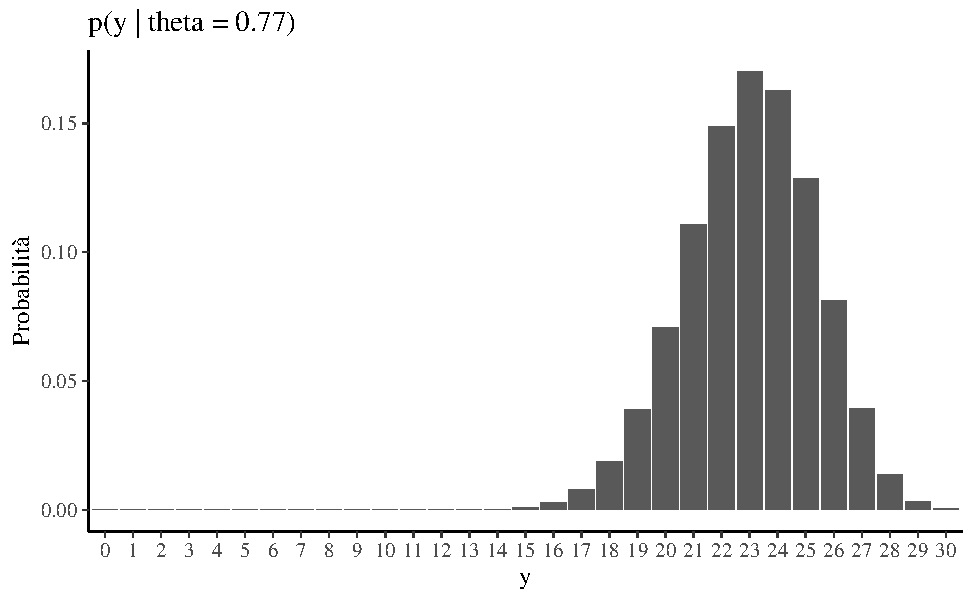
\includegraphics[width=1\linewidth]{ds4psy_files/figure-latex/unnamed-chunk-23-1} 

}

\caption{Istogramma di $M$ campioni casuali $\Theta \sim \mbox{Uniform}(0, 1)$ trasformati in valori $\Phi = \mbox{logit}(\Theta).$ Il profilo limite dell'istogramma è evidenziato nella figura in basso a destra che è stata costruita usando $1\,000\,000$ di osservazioni.}\label{fig:unnamed-chunk-23}
\end{figure}

In un istogramma, l'area di ciascuna barra è proporzionale alla frequenza relativa delle osservazioni in quel'intervallo. Perché tutti gli intervalli hanno la stessa ampiezza, anche l'altezza di ciascuna barra sarà proporzionale alla frequenza relativa delle osservazioni in quel'intervallo.

Nella simulazione, possiamo pensare all'area di ciascuna barra dell'istogramma come alla stima della probabilità che la variabile casuale assuma un valore compreso nell'intervallo considerato. All'aumentare del numero \(M\) di osservazioni, le probabilità stimate si avvicinano sempre di più ai veri valori della probabilità. All'aumentare del numero degli intervalli (quando l'ampiezza \(\Delta\) dell'intervallo \(\rightarrow\) 0), il profilo dell'istogramma tende a diventare una curva continua. Tale curva continua è la funzione di densità di probabilità della variabile casuale. Per l'esempio presente, con \(M =1\,000\,000\), otteniamo il grafico riportato nella figura \ref{fig:hist-dens-example}.

\begin{Shaded}
\begin{Highlighting}[]
\NormalTok{M }\OtherTok{\textless{}{-}} \FloatTok{1e6}
\NormalTok{alpha }\OtherTok{\textless{}{-}} \FunctionTok{logit}\NormalTok{(}\FunctionTok{runif}\NormalTok{(M))}
\NormalTok{density\_limit\_df }\OtherTok{\textless{}{-}} \FunctionTok{data.frame}\NormalTok{(}\AttributeTok{alpha =}\NormalTok{ alpha)}
\NormalTok{density\_limit\_plot }\OtherTok{\textless{}{-}}
\NormalTok{  density\_limit\_df }\SpecialCharTok{\%\textgreater{}\%}
  \FunctionTok{ggplot}\NormalTok{(}\FunctionTok{aes}\NormalTok{(alpha)) }\SpecialCharTok{+}
  \FunctionTok{geom\_histogram}\NormalTok{(}
    \AttributeTok{stat =} \StringTok{"density"}\NormalTok{, }\AttributeTok{n =} \DecValTok{75}\NormalTok{, }\AttributeTok{color =} \StringTok{"black"}\NormalTok{, }\AttributeTok{size =} \FloatTok{0.15}
\NormalTok{  ) }\SpecialCharTok{+}
  \FunctionTok{stat\_function}\NormalTok{(}
    \AttributeTok{fun =}\NormalTok{ dlogis,}
    \AttributeTok{args =} \FunctionTok{list}\NormalTok{(}\AttributeTok{location =} \DecValTok{0}\NormalTok{, }\AttributeTok{scale =} \DecValTok{1}\NormalTok{),}
    \AttributeTok{col =} \StringTok{"black"}\NormalTok{,}
    \AttributeTok{size =} \FloatTok{0.3}
\NormalTok{  ) }\SpecialCharTok{+}
  \FunctionTok{scale\_x\_continuous}\NormalTok{(}
    \AttributeTok{lim =} \FunctionTok{c}\NormalTok{(}\SpecialCharTok{{-}}\DecValTok{9}\NormalTok{, }\DecValTok{9}\NormalTok{),}
    \AttributeTok{breaks =} \FunctionTok{c}\NormalTok{(}\SpecialCharTok{{-}}\DecValTok{6}\NormalTok{, }\SpecialCharTok{{-}}\DecValTok{4}\NormalTok{, }\SpecialCharTok{{-}}\DecValTok{2}\NormalTok{, }\DecValTok{0}\NormalTok{, }\DecValTok{2}\NormalTok{, }\DecValTok{4}\NormalTok{, }\DecValTok{6}\NormalTok{)}
\NormalTok{  ) }\SpecialCharTok{+}
  \FunctionTok{xlab}\NormalTok{(}
    \FunctionTok{expression}\NormalTok{(}\FunctionTok{paste}\NormalTok{(Phi, }\StringTok{" = "}\NormalTok{, }\FunctionTok{logit}\NormalTok{(Theta)))}
\NormalTok{  ) }\SpecialCharTok{+}
  \FunctionTok{ylab}\NormalTok{(}\StringTok{"Frequenza relativa"}\NormalTok{) }\SpecialCharTok{+}
  \FunctionTok{theme}\NormalTok{(}
    \AttributeTok{axis.text.y =} \FunctionTok{element\_blank}\NormalTok{(),}
    \AttributeTok{axis.ticks.y =} \FunctionTok{element\_blank}\NormalTok{()}
\NormalTok{  )}
\NormalTok{density\_limit\_plot}
\end{Highlighting}
\end{Shaded}

\begin{figure}[h]

{\centering 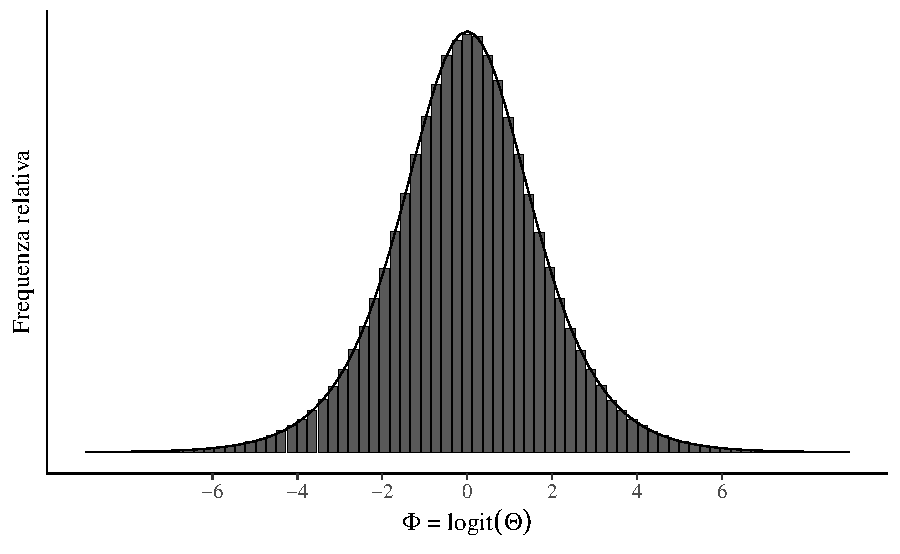
\includegraphics[width=1\linewidth]{ds4psy_files/figure-latex/hist-dens-example-1} 

}

\caption{Istogramma di $M = 1\,000\,000$ campioni casuali $\Theta \sim \mbox{Uniform}(0,1)$ trasformati in valori $\Phi = \mbox{logit}(\Theta)$. La spezzata nera congiunge i punti centrali superiori delle barre dell'istogramma. Nel limite, quando il numero di osservazioni e di barre tende all'infinito, tale spezzata approssima la funzione di densità di probabilità della variabile casuale.}\label{fig:hist-dens-example}
\end{figure}

Nella statistica descrittiva abbiamo già incontrato una rappresentazione che ha lo stesso significato della funzione di densità, ovvero il kernel density plot. La stima della densità del kernel (KDE), infatti, è un modo non parametrico per stimare la funzione di densità di probabilità di una variabile casuale.

\hypertarget{funzione-di-densituxe0-di-probabilituxe0}{%
\section{Funzione di densità di probabilità}\label{funzione-di-densituxe0-di-probabilituxe0}}

Per descrivere le probabilità che possono essere associate ad una variabile casuale continua \(X\) è necessario definire una funzione \(p(X)\) che deve soddisfare le seguenti due proprietà:

\begin{itemize}
\item
  \(p(x) \geq 0, \forall x\), ovvero, l'ordinata della funzione di densità è 0 o positiva;
\item
  \(\int_{-\infty}^{\infty} p(x) \,\operatorname {d}\!x = 1\), ovvero, l'area sottesa dalla \(p(x)\) è unitaria\footnote{Per quel che riguarda la notazione dell'integrale, ovvero \(\int_x \,\operatorname {d}\!x\), rimando alla discussione di S.P. Thompson: \url{https://calculusmadeeasy.org/1.html}};
\item
  \(p(a < x < b) = \int_a^b p(x) \,\operatorname {d}\!x\), se \(a \leq b\), ovvero, l'area sottesa dalla \(p(y)\) tra due punti \(a\) e \(b\) corrisponde alla probabilità che la v.c. \(x\) assuma un valore compresto tra questi due estremi.
\end{itemize}

\emph{Interpretazione.} È possibile che \(p(x) > 1\), quindi una densità di probabilità non può essere interpretata come una probabilità. Piuttosto, la densità \(p(x)\) può essere utilizzata per confrontare la plausibilità relativa di diversi valori \(X\). Considerata una variabile casuale \(X\) di cui è disponibile un insieme di realizzazioni, tanto maggiore è \(p(x_k)\) rispetto a \(p(x_l)\), tanto più grande sarà la nostra certezza che valori nell'intorno di \(x_k\) verranno osservati con maggiore frequenza di valori nell'intorno di \(x_l\).

\hypertarget{exp-val-and-variance-rv}{%
\chapter{Valore atteso e varianza}\label{exp-val-and-variance-rv}}

Spesso risulta utile fornire una rappresentazione sintetica della distribuzione di una variabile casuale attraverso degli indicatori caratteristici piuttosto che fare riferimento ad una sua rappresentazione completa mediante la funzione di ripartizione, o la funzione di massa o di densità di probabilità. Una descrizione più sintetica di una variabile casuale, tramite pochi valori, ci consente di cogliere le caratteristiche essenziali della distribuzione, quali: la posizione, cioè il baricentro della distribuzione di probabilità; la variabilità, cioè la dispersione della distribuzione di probabilità attorno ad un centro; la forma della distribuzione di probabilità, considerando la simmetria e la curtosi (pesantezza delle code). In questo Capitolo introdurremo quegli indici sintetici che descrivono il centro di una distribuzione di probabilità e la sua variabilità.

\hypertarget{valore-atteso}{%
\section{Valore atteso}\label{valore-atteso}}

Quando vogliamo conoscere il comportamento tipico di una variabile casuale spesso vogliamo sapere qual è il suo ``valore tipico''. La nozione di ``valore tipico'', tuttavia, è ambigua. Infatti, essa può essere definita in almeno tre modi diversi:

\begin{itemize}
\tightlist
\item
  la \emph{media} (somma dei valori divisa per il numero dei valori),
\item
  la \emph{mediana} (il valore centrale della distribuzione, quando la variabile è ordinata in senso crescente o decrescente),
\item
  la \emph{moda} (il valore che ricorre più spesso).
\end{itemize}

Per esempio, la media di \(\{3, 1, 4, 1, 5\}\) è \(\frac{3+1+4+1+5}{5} = 2.8\), la mediana è \(3\) e la moda è \(1\). Tuttavia, la teoria delle probabilità si occupa di variabili casuali piuttosto che di sequenze di numeri. Diventa dunque necessario precisare che cosa intendiamo per ``valore tipico'' quando facciamo riferimento alle variabili casuali. Giungiamo così alla seguente definizione.

\begin{definition}
Sia \(Y\) è una variabile casuale discreta che assume i valori \(y_1, \dots, y_n\) con distribuzione \(p(y)\), ossia

\[
P(Y = y_i) = p(y_i),
\]

per definizione il \emph{valore atteso} di \(Y\), \(\E(Y)\), è

\begin{equation}
\E(Y) = \sum_{i=1}^n y_i \cdot p(y_i).
\label{eq:expval-discr}
\end{equation}
\end{definition}

A parole: il valore atteso (o speranza matematica, o aspettazione, o valor medio) di una variabile casuale è definito come la somma di tutti i valori che la variabile casuale può prendere, ciascuno pesato dalla probabilità con cui il valore è preso.

\begin{exercise}
Calcoliamo il valore atteso della variabile casuale \(Y\) corrispondente al lancio di una moneta equilibrata (testa: \emph{Y} = 1; croce: \emph{Y} = 0).

\[
\E(Y) = \sum_{i=1}^{2} y_i \cdot P(y_i) = 0 \cdot \frac{1}{5} + 1 \cdot \frac{1}{5} = 0.5.
\]
\end{exercise}

\begin{exercise}
Supponiamo ora che \emph{Y} sia il risultato del lancio di un dado equilibrato. Il valore atteso di \emph{Y} diventa:

\[
\E(Y) = \sum_{i=1}^{6} y_i \cdot P(y_i) = 1 \cdot \frac{1}{6} + 2 \cdot \frac{1}{6} + \dots + 6 \cdot \frac{1}{6} = \frac{21}{6} = 3.5.
\]
\end{exercise}

\hypertarget{interpretazione}{%
\subsection{Interpretazione}\label{interpretazione}}

Che interpretazione può essere assegnata alla nozione di valore atteso? Bruno de Finetti adottò lo stesso termine di \emph{previsione} (e lo stesso simbolo) tanto per la probabilità che per la speranza matematica. Si può pertanto dire che, dal punto di vista bayesiano, la speranza matematica è l'estensione naturale della nozione di probabilità soggettiva.

\hypertarget{proprietuxe0-del-valore-atteso}{%
\subsection{Proprietà del valore atteso}\label{proprietuxe0-del-valore-atteso}}

La proprietà più importante del valore atteso è la linearità: il valore atteso di una somma di variabili casuali è uguale alla somma dei lori rispettivi valori attesi:

\begin{equation}
\E(X + Y) = \E(X) + \E(Y).
\label{eq:prop-expval-linearity}
\end{equation}

La \eqref{eq:prop-expval-linearity} sembra ragionevole quando \(X\) e \(Y\) sono indipendenti, ma è anche vera quando \(X\) e \(Y\) sono associati. Abbiamo anche che

\begin{equation}
\E(cY) = c \E(Y).
\label{eq:prop-expval-const}
\end{equation}

La \eqref{eq:prop-expval-const} ci dice che possiamo estrarre una costante dall'operatore di valore atteso. Tale proprietà si estende a qualunque numero di variabili casuali. Infine, se due variabili casuali \(X\) e \(Y\) sono indipendenti, abbiamo che

\begin{equation}
\E(X Y) = \E(X) \E(Y). 
\label{eq:expval-prod-ind-rv}
\end{equation}

\begin{exercise}
Si considerino le seguenti variabili casuali: \(Y\), ovvero il numero che si ottiene dal lancio di un dado equilibrato, e \(Y\), il numero di teste prodotto dal lancio di una moneta equilibrata. Poniamoci il problema di trovare il valore atteso di \(X+Y\).

Per risolvere il problema iniziamo a costruire lo spazio campionario dell'esperimento casuale consistente nel lancio di un dado e di una moneta.

\begin{longtable}[]{@{}ccccccc@{}}
\toprule
\(x/ y\) & 1 & 2 & 3 & 4 & 5 & 6 \\
\midrule
\endhead
0 & (0, 1) & (0, 2) & (0, 3) & (0, 4) & (0, 5) & (0, 6) \\
1 & (1, 1) & (1, 2) & (1, 3) & (1, 4) & (1, 5) & (1, 6) \\
\bottomrule
\end{longtable}

\noindent ovvero

\begin{longtable}[]{@{}ccccccc@{}}
\toprule
\(x/ y\) & 1 & 2 & 3 & 4 & 5 & 6 \\
\midrule
\endhead
0 & 1 & 2 & 3 & 4 & 5 & 6 \\
1 & 2 & 3 & 4 & 5 & 6 & 7 \\
\bottomrule
\end{longtable}

\noindent Il risultato del lancio del dado è indipendente dal risultato del lancio della moneta. Pertanto, ciascun evento elementare dello spazio campionario avrà la stessa probabilità di verificarsi, ovvero \(Pr(\omega) = \frac{1}{12}\). Il valore atteso di \(X+Y\) è dunque uguale a:

\[
\E(X+Y) = 1 \cdot \frac{1}{12} + 2 \cdot \frac{1}{12} + \dots + 7 \cdot \frac{1}{12} = 4.0.
\]

Lo stesso risultato si ottiene nel modo seguente:

\[
\E(X+Y) = \E(X) + E(Y) = 3.5 + 0.5 = 4.0.
\]
\end{exercise}

\begin{exercise}
Si considerino le variabili casuali \(X\) e \(Y\) definite nel caso del lancio di tre monete equilibrate, dove \(X\) conta il numero delle teste nei tre lanci e \(Y\) conta il numero delle teste al primo lancio. Si calcoli il valore atteso del prodotto delle variabili casuali \(X\) e \(Y\).

La distribuzione di probabilità congiunta \(P(X, Y)\) è fornita nella tabella seguente.

\begin{longtable}[]{@{}cccc@{}}
\toprule
\(x/ y\) & 0 & 1 & \(p(Y)\) \\
\midrule
\endhead
0 & 1/8 & 0 & 1/8 \\
1 & 2/8 & 1/8 & 3/8 \\
2 & 1/8 & 2/8 & 3/8 \\
3 & 0 & 1/8 & 1/8 \\
\(p(y)\) & 4/8 & 4/8 & 1.0 \\
\bottomrule
\end{longtable}

\noindent Il calcolo del valore atteso di \(XY\) si riduce a

\[
\E(XY) = 1 \cdot \frac{1}{8} + 2 \cdot \frac{2}{8} + 3 \cdot \frac{1}{8} = 1.0.
\]

Si noti che le variabili casuali \(Y\) e \(Y\) non sono indipendenti. Dunque non possiamo usare la proprietà \ref{thm:prodindrv}. Infatti, il valore atteso di \(X\) è

\[
\E(X) = 1 \cdot \frac{3}{8} + 2 \cdot \frac{3}{8} + 3 \cdot \frac{1}{8} = 1.5
\]

e il valore atteso di \(Y\) è

\[
\E(Y) = 0 \cdot \frac{4}{8} + 1 \cdot \frac{4}{8} = 0.5.
\] Dunque

\[
1.5 \cdot 0.5 \neq 1.0.
\]
\end{exercise}

\hypertarget{variabili-casuali-continue}{%
\subsection{Variabili casuali continue}\label{variabili-casuali-continue}}

Nel caso di una variabile casuale continua \(Y\) il valore atteso diventa:

\begin{equation}
\E(Y) = \int_{-\infty}^{+\infty} y p(y) \,\operatorname {d}\!y
\label{eq:def-ev-rv-cont}
\end{equation}

Anche in questo caso il valore atteso è una media ponderata della \(y\), nella quale ciascun possibile valore \(y\) è ponderato per il corrispondente valore della densità \(p(y)\). Possiamo leggere l'integrale pensando che \(y\) rappresenti l'ampiezza delle barre infinitamente strette di un istogramma, con la densità \(p(y)\) che corrisponde all'altezza di tali barre e la notazione \(\int_{-\infty}^{+\infty}\) che corrisponde ad una somma.

Un'altra misura di tendenza centrale delle variabili casuali continue è la moda. La moda della \(Y\) individua il valore \(y\) più plausibile, ovvero il valore \(y\) che massimizza la funzione di densità \(p(y)\):

\begin{equation}
\Mo(Y) = \argmax_y p(y).
\label{eq:def-mode}
\end{equation}

\hypertarget{varianza}{%
\section{Varianza}\label{varianza}}

La seconda più importante proprietà di una variabile casuale, dopo che conosciamo il suo valore atteso, è la \emph{varianza}.

\begin{definition}
Se \(Y\) è una variabile casuale discreta con distribuzione \(p(y)\), per definizione la varianza di \(Y\), \(\Var(Y)\), è

\begin{equation}
\Var(Y) = \E\Big[\big(Y - \E(Y)\big)^2\Big].
\label{eq:def-var-rv}
\end{equation}
\end{definition}

A parole: la varianza è la deviazione media quadratica della variabile dalla sua media.\footnote{Data una variabile casuale \(Y\) con valore atteso \(\E(Y)\), le ``distanze'' tra i valori di \(Y\) e il valore atteso \(\E(Y)\) definiscono la variabile casuale \(Y - \E(Y)\) chiamata \emph{scarto}, oppure \emph{deviazione} oppure \emph{variabile casuale centrata}. La variabile \(Y - \E(Y)\) equivale ad una traslazione di sistema di riferimento che porta il valore atteso nell'origine degli assi. Si può dimostrare facilmente che il valore atteso della variabile scarto \(Y - \E(Y)\) vale zero, dunque la media di tale variabile non può essere usata per quantificare la ``dispersione'' dei valori di \(Y\) relativamente al suo valore medio. Occorre rendere sempre positivi i valori di \(Y - \E(Y)\) e tale risultato viene ottenuto considerando la variabile casuale \(\left(Y - \E(Y)\right)^2\).} Se denotiamo \(\E(Y) = \mu\), la varianza \(\Var(Y)\) diventa il valore atteso di \((Y - \mu)^2\).

\begin{exercise}
Posta \(S\) uguale alla somma dei punti ottenuti nel lancio di due dadi equilibrati, poniamoci il problema di calcolare la varianza di \(S\).

La variabile casuale \(S\) ha la seguente distribuzione di probabilità:

\begin{longtable}[]{@{}cccccccccccc@{}}
\toprule
\(s\) & 2 & 3 & 4 & 5 & 6 & 7 & 8 & 9 & 10 & 11 & 12 \\
\midrule
\endhead
\(P(S = s)\) & \(\frac{1}{36}\) & \(\frac{2}{36}\) & \(\frac{3}{36}\) & \(\frac{4}{36}\) & \(\frac{5}{36}\) & \(\frac{6}{36}\) & \(\frac{5}{36}\) & \(\frac{4}{36}\) & \(\frac{3}{36}\) & \(\frac{2}{36}\) & \(\frac{1}{36}\) \\
\bottomrule
\end{longtable}

\noindent Essendo \(\E(S) = 7\), la varianza diventa

\begin{align}
\Var(S) &= \sum \left(S- \mathbb{E}(S)\right)^2 \cdot P(S) \notag\\
&= (2 - 7)^2 \cdot 0.0278 + (3-7)^2 \cdot 0.0556 + \dots + (12 - 7)^2 \cdot 0.0278 \notag\\
&= 5.8333.\notag
\end{align}
\end{exercise}

\hypertarget{formula-alternativa-per-la-varianza}{%
\subsection{Formula alternativa per la varianza}\label{formula-alternativa-per-la-varianza}}

C'è un modo più semplice per calcolare la varianza:

\begin{align}
\E\Big[\big(X - \E(Y)\big)^2\Big] &= \E\big(X^2 - 2X\E(Y) + \E(Y)^2\big)\notag\\
&= \E(Y^2) - 2\E(Y)\E(Y) + \E(Y)^2,\notag
\end{align}

dato che \(\E(Y)\) è una costante; pertanto

\begin{equation}
\Var(Y) = \E(Y^2) - \big(\E(Y) \big)^2.
\label{eq:def-alt-var-rv}
\end{equation}

A parole: la varianza è la media dei quadrati meno il quadrato della media.

\begin{exercise}
Consideriamo la variabile casuale \(Y\) che corrisponde al numero di teste che si osservano nel lancio di una moneta truccata con probabilità di testa uguale a 0.8. Il valore atteso di \(Y\) è

\[
\E(Y) = 0 \cdot 0.2 + 1 \cdot 0.8 = 0.8.
\] Usando la formula tradizionale della varianza otteniamo:

\[
\Var(Y) = (0 - 0.8)^2 \cdot 0.2 + (1 - 0.8)^2 \cdot 0.8 = 0.16.
\] Lo stesso risultato si trova con la formula alternativa della varianza. Il valore atteso di \(Y^2\) è

\[
\E(Y^2) = 0^2 \cdot 0.2 + 1^2 * 0.8 = 0.8.
\] e la varianza diventa

\[
\Var(Y) = \E(Y^2) - \big(\E(Y) \big)^2 = 0.8 - 0.8^2 = 0.16.
\]
\end{exercise}

\hypertarget{variabili-casuali-continue-1}{%
\subsection{Variabili casuali continue}\label{variabili-casuali-continue-1}}

Nel caso di una variabile casuale continua \(Y\), la varianza diventa:

\begin{equation}
\Var(Y) = \int_{-\infty}^{+\infty} \large[y - \E(Y)\large]^2 p(y) \,\operatorname {d}\!y
\label{eq:def-var-rv-cont}
\end{equation}

Come nel caso discreto, la varianza di una v.c. continua \(y\) misura approssimativamente la distanza al quadrato tipica o prevista dei possibili valori \(y\) dalla loro media.

\hypertarget{deviazione-standard}{%
\section{Deviazione standard}\label{deviazione-standard}}

Quando lavoriamo con le varianze, i termini sono innalzati al quadrato e quindi i numeri possono diventare molto grandi (o molto piccoli). Per trasformare nuovamente i valori nell'unità di misura della scala originaria si prende la radice quadrata. Il valore risultante viene chiamato \emph{deviazione standard} e solitamente è denotato dalla lettera greca \(\sigma\).

\begin{definition}
Si definisce scarto quadratico medio (o deviazione standard o scarto tipo) la radice quadrata della varianza:

\begin{equation}
\sigma_Y = \sqrt{\Var(Y)}.
\label{eq:def-sd}
\end{equation}
\end{definition}

Interpretiamo la deviazione standard di una variabile casuale come nella statistica descrittiva: misura approssimativamente la distanza tipica o prevista dei possibili valori \(y\) dalla loro media.

\begin{exercise}
Per i dadi equilibrati dell'esempio precedente, la deviazione standard della variabile casuale \(S\) è uguale a \(\sqrt{5.833} = 2.415\).
\end{exercise}

\hypertarget{standardizzazione}{%
\section{Standardizzazione}\label{standardizzazione}}

\begin{definition}
Data una variabile casuale \(Y\), si dice variabile standardizzata di \(Y\) l'espressione

\begin{equation}
Z = \frac{Y - \E(Y)}{\sigma_Y}.
\label{eq:standardization}
\end{equation}
\end{definition}

Solitamente, una variabile standardizzata viene denotata con la lettera \(Z\).

\hypertarget{momenti-di-variabili-casuali}{%
\section{Momenti di variabili casuali}\label{momenti-di-variabili-casuali}}

\begin{definition}
Si chiama \emph{momento} di ordine \(q\) di una v.c. \(X\), dotata di densità \(p(x)\), la quantità

\begin{equation}
\E(X^q) = \int_{-\infty}^{+\infty} x^q p(x) \; dx.
\end{equation}

Se \(X\) è una v.c. discreta, i suoi momenti valgono:

\begin{equation}
\E(X^q) = \sum_i x_i^q p(x_i).
\end{equation}
\end{definition}

I momenti sono importanti parametri indicatori di certe proprietà di \(X\). I più noti sono senza dubbio quelli per \(q = 1\) e \(q = 2\). Il momento del primo ordine corrisponde al valore atteso di \(X\). Spesso i momenti di ordine superiore al primo vengono calcolati rispetto al valor medio di \(X\), operando una traslazione \(x_0 = x − \E(X)\) che individua lo scarto dalla media. Ne deriva che il momento centrale di ordine 2 corrisponde alla varianza.

\hypertarget{funzione-di-ripartizione}{%
\section{Funzione di ripartizione}\label{funzione-di-ripartizione}}

Il concetto di funzione di ripartizione è molto importante nella teoria della probabilità, sia nel caso discreto, sia in quello continuo. L'insieme \(\{\omega: Y \leq y\}\) è un evento in \(\Omega\) e si può scrivere \((Y \leq y)\). A tale evento è possibile assegnare una probabilità \(P(Y \leq y)\) che, al variare di \(y \in \mathbb{R}\), definisce la funzione di ripartizione della variabile casuale \(Y\).

\begin{definition}
Si chiama \emph{funzione di ripartizione} o \emph{funzione di distribuzione} della variabile casuale \(X\) la funzione \(F(X)\) definita da

\begin{equation}
F(X) \triangleq P(X \le x), \qquad x \in \mathbb{R}.
\label{eq:funrip}
\end{equation}
\end{definition}

Detto a parole: la funzione di distribuzione cumulata, o funzione di ripartizione di \(X\), misura la probabilità che \(X\) assuma valori minori o uguali al valore \(x\).

La funzione di ripartizione è sempre non negativa, monotona non decrescente tra \(0\) e \(1\), tale che:

\[
\lim_{x \to -\infty} F_x(X) = F_X(-\infty) = 0, \quad \lim_{x \to +\infty} F_X(X) = F_X(+\infty) = 1.
\]

\begin{exercise}
Consideriamo l'esperimento casuale corrispondente al lancio di due monete. Sia \(X\) il numero di volte in cui esce testa. La distribuzione di probabilità di \(X\) è:

\[
P(X) = 
\begin{cases}
    0, & 0.25,\\
    1, & 0.50,\\
    2, & 0.25.
\end{cases}
\] La funzione di ripartizione di \(X\) è:

\[
    F(X) = 
\begin{cases}
    0,   & \text{se } x < 0,\\
    1/4, & \text{se } 0 \leq x < 1,\\
    3/4, & \text{se } 1 \leq x < 2,\\
     1,  & \text{se } 2 \leq x.
\end{cases}
\]

Il valore della funzione di ripartizione in corrispondenza di \(x = 1.5\), ad esempio, è:

\[
F(1.5) = P(X \leq 1.5) = P(X=0) + P(X=1) = \frac{1}{4} + \frac{2}{4} = \frac{3}{4}.
\]
\end{exercise}

\mainmatter

\hypertarget{part-distribuzioni-teoriche-di-probabilituxe0}{%
\part{Distribuzioni teoriche di probabilità}\label{part-distribuzioni-teoriche-di-probabilituxe0}}

\hypertarget{distr-rv-discr}{%
\chapter{Distribuzioni di v.c. discrete}\label{distr-rv-discr}}

In questo Capitolo verranno esaminate le principali distribuzioni di probabilità delle variabili casuali discrete. Un esperimento casuale che può dare luogo a solo due possibili esiti (successo, insuccesso) è modellabile con una variabile casuale di Bernoulli. Una sequenza di prove di Bernoulli costituisce un processo Bernoulliano. Il numero di successi dopo \(n\) prove di Bernoulli corrisponde ad una variabile casuale che segue la legge binomiale. La distribuzione binomiale risulta da un insieme di prove di Bernoulli solo se il numero totale \(n\) è fisso per disegno. Se il numero di prove è esso stesso una variabile casuale, allora il numero di successi nella corrispondente sequenza di prove bernoulliane segue al distribuzione di Poisson.

\hypertarget{una-prova-bernoulliana}{%
\section{Una prova Bernoulliana}\label{una-prova-bernoulliana}}

Se un esperimento casuale ha solo due esiti possibili, allora le repliche indipendenti di questo esperimento sono chiamate ``prove Bernoulliane'' (il lancio di una moneta è il tipico esempio).

\begin{definition}
Viene detta variabile di Bernoulli una variabile casuale discreta \(Y = \{0, 1\}\) con la seguente distribuzione di probabilità:

\[
P(Y \mid \theta) =
  \begin{cases}
    \theta     & \text{se $Y = 1$}, \\
    1 - \theta & \text{se $Y = 0$},
  \end{cases}
\]

con \(0 \leq \theta \leq 1\). Convenzionalmente l'evento \(\{Y = 1\}\) con probabilità \(\theta\) viene chiamato ``successo'' mentre l'evento \(\{Y = 0\}\) con probabilità \(1-\theta\) viene chiamato ``insuccesso''.
\end{definition}

Applicando l'operatore di valore atteso e di varianza, otteniamo

\begin{align}
\E(Y) &= 0 \cdot Pr(Y=0) + 1 \cdot Pr(Y=1) = \theta, \\
\Var(Y) &= (0 - \theta)^2 \cdot Pr(Y=0) + (1 - \theta)^2 \cdot rP(Y=1) = \theta(1-\theta).
\label{eq:ev-var-bern}
\end{align}

Scriviamo \(Y \sim \mathcal{B}(\theta)\) per indicare che la variabile casuale \(Y\) ha una distribuzione Bernoulliana di parametro \(\theta\).

\begin{exercise}
Nel caso del lancio di una moneta equilibrata la variabile casuale di Bernoulli assume i valori \(0\) e \(1\). La distribuzione di massa di probabilità è pari a \(\frac{1}{2}\) in corrispondenza di entrambi iv valori. La funzione di distribuzione vale \(\frac{1}{2}\) per \(Y = 0\) e \(1\) per \(Y = 1\).
\end{exercise}

\hypertarget{una-sequenza-di-prove-bernoulliane}{%
\section{Una sequenza di prove Bernoulliane}\label{una-sequenza-di-prove-bernoulliane}}

La distribuzione binomiale è rappresentata dall'elenco di tutti i possibili numeri di successi \(Y = \{0, 1, 2, \dots n\}\) che possono essere osservati in \(n\) prove Bernoulliane indipendenti di probabilità \(\theta\), a ciascuno dei quali è associata la relativa probabilità. Esempi di una distribuzione binomiale sono i risultati di una serie di lanci di una stessa moneta o di una serie di estrazioni da un'urna (con reintroduzione). La distribuzione binomiale di parametri \(n\) e \(\theta\) è in realtà una famiglia di distribuzioni: al variare dei parametri \(\theta\) e \(n\) variano le probabilità.

\begin{definition}
La probabilità di ottenere \(y\) successi e \(n-y\) insuccessi in \(n\) prove Bernoulliane è data dalla distribuzione binomiale:

\begin{align}
P(Y=y) &= \binom{n}{y} \theta^{y} (1-\theta)^{n-y} \notag \\
&= \frac{n!}{y!(n-y)!} \theta^{y} (1-\theta)^{n-y}, 
\label{eq:binomialdistribution}
\end{align}

dove \(n\) = numero di prove Bernoulliane, \(\theta\) = probabilità di successo in ciascuna prova e \(y\) = numero di successi.
\end{definition}

\begin{proof}
La \eqref{eq:binomialdistribution} può essere derivata nel modo seguente. Indichiamo con \(S\) il successo e con \(I\) l'insuccesso di ciascuna prova. Una sequenza di \(n\) prove Bernoulliane darà come esito una sequenza di \(n\) elementi \(S\) e \(I\). Ad esempio, una sequenza che contiene \(y\) successi è la seguente:

\[
\overbrace{SS\dots S}^\text{$y$ volte} \overbrace{II\dots I}^\text{$n-y$ volte}
\] Essendo \(\theta\) la probabilità di \(S\) e \(1-\theta\) la probabilità di \(I\), la probabilità di ottenere la specifica sequenza riportata sopra è

\begin{equation}
\overbrace{\theta \theta\dots \theta}^\text{$y$ volte} \overbrace{(1-\theta)(1-\theta)\dots (1-\theta)}^\text{$n-y$ volte} = \theta^y \cdot (1-\theta)^{n-y}.
\label{eq:demo-bino-kernel}
\end{equation}

Non siamo però interessati alla probabilità di una \emph{specifica} sequenza di \(S\) e \(I\) ma, bensì, alla probabilità di osservare una \emph{qualsiasi} sequenza di \(y\) successi in \(n\) prove. In altre parole, vogliamo la probabilità dell'unione di tutti gli eventi corrispondenti a \(y\) successi in \(n\) prove.

È immediato notare che una qualsiasi altra sequenza contenente esattamente \(y\) successi avrà sempre come probabilità \(\theta^y \cdot (1-\theta)^{n-y}\): il prodotto infatti resta costante anche se cambia l'ordine dei fattori.\footnote{Viene detta \emph{scambiabilità} la proprietà per cui l'ordine con cui compiamo le osservazioni è irrilevante per l'assegnazione delle probabilità.} Per trovare il risultato cercato dobbiamo moltiplicare la \eqref{eq:demo-bino-kernel} per il numero di sequenze possibili di \(y\) successi in \(n\) prove.

Il numero di sequenze che contengono esattamente \(y\) successi in \(n\) prove. La risposta è fornita dal coefficiente binomiale\footnote{La derivazione della formula del coefficiente binomiale è fornita nell'Appendice \ref{derivazione-coef-binom}.}:

\begin{equation}
\binom{n}{y} = \frac{n!}{y!(n-y)!},
\label{eq:binomial-coefficient}
\end{equation}

dove il simbolo \(n!\) si legge \(n\) fattoriale ed è uguale al prodotto di \(n\) numeri interi decrescenti a partire da \(n\). Per definizione \(0! = 1\).

Essendo la probabilità dell'unione di \(K\) elementi incompatibili uguale alla somma delle loro rispettive probabilità, e dato che le sequenze di \(y\) successi in \(n\) prove hanno tutte la stessa probabilità, per trovare la formula della distributione binomiale \eqref{eq:binomialdistribution} è sufficiente moltiplicare la \eqref{eq:demo-bino-kernel} per la \eqref{eq:binomial-coefficient}.
\end{proof}

La distribuzione di probabilità di alcune distribuzioni binomiali, per due valori di \(n\) e \(\theta\), è fornita nella figura \ref{fig:example-binomial-distr}.

\begin{figure}[h]

{\centering 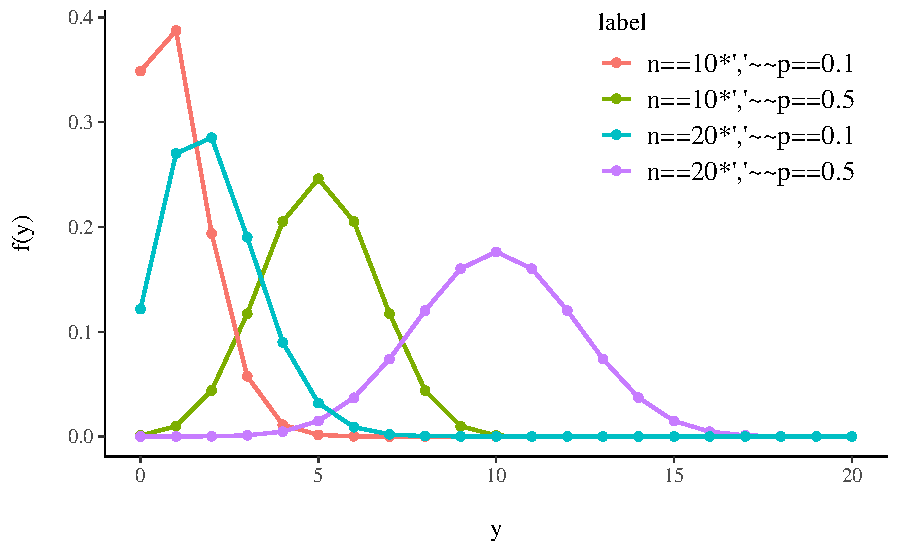
\includegraphics{ds4psy_files/figure-latex/example-binomial-distr-1} 

}

\caption{Alcune distribuzioni binomiali. Nella figura, il parametro $\theta$ è indicato con $p$.}\label{fig:example-binomial-distr}
\end{figure}

\begin{exercise}

Usando la \eqref{eq:binomialdistribution}, si trovi la probabilità di \(y = 2\) successi in \(n = 4\) prove Bernoulliane indipendenti con \(\theta = 0.2\)

\[
\begin{aligned}
P(Y=2) &= \frac{4!}{2!(4-2)!} 0.2^{2} (1-0.2)^{4-2} \notag  \\
 &= \frac{4 \cdot 3 \cdot 2 \cdot 1}{(2 \cdot 1)(2 \cdot 1)}
0.2^{2} 0.8^{2} = 0.1536. \notag
\end{aligned}
\]

Ripetendo i calcoli per i valori \(y = 0, \dots, 4\) troviamo la distribuzione binomiale di parametri \(n = 4\) e \(\theta = 0.2\):

\begin{longtable}[]{@{}cc@{}}
\toprule
y & P(Y = y) \\
\midrule
\endhead
0 & 0.4096 \\
1 & 0.4096 \\
2 & 0.1536 \\
3 & 0.0256 \\
4 & 0.0016 \\
sum & 1.0 \\
\bottomrule
\end{longtable}

Lo stesso risultato si ottiene usando la sequente istruzione \R:

\begin{Shaded}
\begin{Highlighting}[]
\FunctionTok{dbinom}\NormalTok{(}\DecValTok{0}\SpecialCharTok{:}\DecValTok{4}\NormalTok{, }\DecValTok{4}\NormalTok{, }\FloatTok{0.2}\NormalTok{)}
\CommentTok{\#\textgreater{} [1] 0.4096 0.4096 0.1536 0.0256 0.0016}
\end{Highlighting}
\end{Shaded}

\end{exercise}

\begin{exercise}

Lanciando \(5\) volte una moneta onesta, qual è la probabilità che esca testa almeno tre volte?

In \R, la soluzione si trova con

\begin{Shaded}
\begin{Highlighting}[]
\FunctionTok{dbinom}\NormalTok{(}\DecValTok{3}\NormalTok{, }\DecValTok{5}\NormalTok{, }\FloatTok{0.5}\NormalTok{) }\SpecialCharTok{+} \FunctionTok{dbinom}\NormalTok{(}\DecValTok{4}\NormalTok{, }\DecValTok{5}\NormalTok{, }\FloatTok{0.5}\NormalTok{) }\SpecialCharTok{+} \FunctionTok{dbinom}\NormalTok{(}\DecValTok{5}\NormalTok{, }\DecValTok{5}\NormalTok{, }\FloatTok{0.5}\NormalTok{)}
\CommentTok{\#\textgreater{} [1] 0.5}
\end{Highlighting}
\end{Shaded}

Alternativamente, possiamo trovare la probabilità dell'evento complementare a quello definito dalla funzione di ripartizione calcolata mediante \texttt{pbinom()}, ovvero

\begin{Shaded}
\begin{Highlighting}[]
\DecValTok{1} \SpecialCharTok{{-}} \FunctionTok{pbinom}\NormalTok{(}\DecValTok{2}\NormalTok{, }\DecValTok{5}\NormalTok{, }\FloatTok{0.5}\NormalTok{)}
\CommentTok{\#\textgreater{} [1] 0.5}
\end{Highlighting}
\end{Shaded}

\end{exercise}

\hypertarget{valore-atteso-e-deviazione-standard}{%
\subsection{Valore atteso e deviazione standard}\label{valore-atteso-e-deviazione-standard}}

La media (numero atteso di successi in \(n\) prove) e la deviazione standard di una distribuzione binomiale sono molto semplici:

\begin{align}
\mu    &= n\theta,  \notag \\
\sigma &= \sqrt{n\theta(1-\theta)}.
\end{align}

\begin{proof}
Essendo \(Y\) la somma di \(n\) prove Bernoulliane indipendenti \(Y_i\), è facile vedere che \begin{align}
\E(Y) &= \E \left( \sum_{i=1}^n Y_i \right) = \sum_{i=1}^n \E(Y_i) = n\theta, \\
\Var(Y) &= \Var \left( \sum_{i=1}^n Y_i \right) = \sum_{i=1}^n \Var(Y_i) = n \theta (1-\theta).
\end{align}
\end{proof}

\begin{exercise}
Si trovino il valore atteso e la varianza del lancio di quattro monete con probabilità di successo pari a \(\theta = 0.2\).

Il valore atteso è \(\mu = n\theta = 4 \cdot 0.2 = 0.8.\) Ciò significa che, se l'esperimento casuale venisse ripetuto infinite volte, l'esito testa verrebbe osservato un numero medio di volte pari a 0.8. La varianza è \(n \theta (1-\theta) = 4 \cdot(1 - 0.2) = 0.8\).\footnote{L'eguaglianza di \(\mu\) e \(\sigma\) è solo una peculiarità di questo esempio.}
\end{exercise}

\hypertarget{distribuzione-di-poisson}{%
\section{Distribuzione di Poisson}\label{distribuzione-di-poisson}}

La distribuzione di Poisson è una distribuzione di probabilità discreta che esprime le probabilità per il numero di eventi che si verificano successivamente ed indipendentemente in un dato intervallo di tempo, sapendo che mediamente se ne verifica un numero \(\lambda\). La distribuzione di Poisson serve dunque per contare il numero di volte in cui un evento ha luogo in un determinato intervallo di tempo. La stessa distribuzione può essere estesa anche per contare gli eventi che hanno luogo in una determinata porzione di spazio.

\begin{definition}
La distribuzione di Poisson può essere intesa come limite della distribuzione binomiale, dove la probabilità di successo \(\theta\) è pari a \(\frac{\lambda}{n}\) con \(n\) che tende a \(\infty\):

\begin{equation}
\lim_{y \rightarrow \infty} \binom{n}{y} \theta^y (1-\theta)^{n-y} = \frac{\lambda^y}{y!}e^{-\lambda}.
\end{equation}
\end{definition}

Alcune distribuzioni di Poisson sono riportate nella figura \ref{fig:examples-poisson-distrib}.

\begin{figure}[h]

{\centering 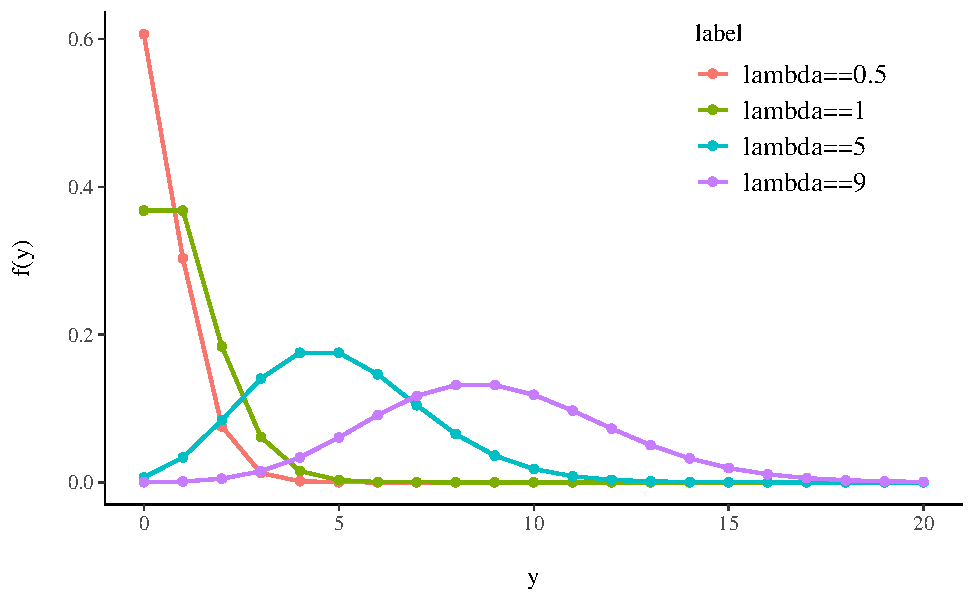
\includegraphics{ds4psy_files/figure-latex/examples-poisson-distrib-1} 

}

\caption{Alcune distribuzioni di Poisson.}\label{fig:examples-poisson-distrib}
\end{figure}

\begin{exercise}

Supponiamo che un evento accada 300 volte all'ora e si vuole determinare la probabilità che in un minuto accadano esattamente 3 eventi.

Il numero medio di eventi in un minuto è pari a

\begin{Shaded}
\begin{Highlighting}[]
\NormalTok{lambda }\OtherTok{\textless{}{-}} \DecValTok{300} \SpecialCharTok{/} \DecValTok{60}
\NormalTok{lambda}
\CommentTok{\#\textgreater{} [1] 5}
\end{Highlighting}
\end{Shaded}

\noindent Quindi la probabilità che in un minuto si abbiano 3 eventi è pari a

\begin{Shaded}
\begin{Highlighting}[]
\NormalTok{y }\OtherTok{\textless{}{-}} \DecValTok{3}
\NormalTok{(lambda}\SpecialCharTok{\^{}}\NormalTok{y }\SpecialCharTok{/} \FunctionTok{factorial}\NormalTok{(y)) }\SpecialCharTok{*} \FunctionTok{exp}\NormalTok{(}\SpecialCharTok{{-}}\NormalTok{lambda)}
\CommentTok{\#\textgreater{} [1] 0.1404}
\end{Highlighting}
\end{Shaded}

\end{exercise}

\begin{exercise}

Per i dati dell'esempio precedente, si trovi la probabilità che un evento accada almeno 8 volte in un minuto.

La probabilità cercata è

\[
p(y \geq 8) = 1 - p (y \leq 7) = 1- \sum_{i = 0}^7 \frac{\lambda^7}{7!}e^{-\lambda},
\] \noindent con \(\lambda = 5\).

Svolgendo i calcoli in \R otteniamo:

\begin{Shaded}
\begin{Highlighting}[]
\DecValTok{1} \SpecialCharTok{{-}} \FunctionTok{ppois}\NormalTok{(}\AttributeTok{q =} \DecValTok{7}\NormalTok{, }\AttributeTok{lambda =} \DecValTok{5}\NormalTok{)}
\CommentTok{\#\textgreater{} [1] 0.1334}
\FunctionTok{ppois}\NormalTok{(}\AttributeTok{q =} \DecValTok{7}\NormalTok{, }\AttributeTok{lambda =} \DecValTok{5}\NormalTok{, }\AttributeTok{lower.tail =} \ConstantTok{FALSE}\NormalTok{)}
\CommentTok{\#\textgreater{} [1] 0.1334}
\end{Highlighting}
\end{Shaded}

\end{exercise}

\begin{exercise}

Sapendo che un evento avviene in media 6 volte al minuto, si calcoli (a) la probabilità di osservare un numero di eventi uguale o inferiore a 3 in un minuto, e (b) la probabilità di osservare esattamente 2 eventi in 30 secondi.

\begin{enumerate}
\def\labelenumi{(\alph{enumi})}
\tightlist
\item
  In questo caso \(\lambda = 6\) e la probabilità richiesta è
\end{enumerate}

\begin{Shaded}
\begin{Highlighting}[]
\FunctionTok{ppois}\NormalTok{(}\AttributeTok{q =} \DecValTok{3}\NormalTok{, }\AttributeTok{lambda =} \DecValTok{6}\NormalTok{, }\AttributeTok{lower.tail =} \ConstantTok{TRUE}\NormalTok{)}
\CommentTok{\#\textgreater{} [1] 0.1512}
\end{Highlighting}
\end{Shaded}

\begin{enumerate}
\def\labelenumi{(\alph{enumi})}
\setcounter{enumi}{1}
\tightlist
\item
  In questo caso \(\lambda = 6 / 2\) e la probabilità richiesta è
\end{enumerate}

\begin{Shaded}
\begin{Highlighting}[]
\FunctionTok{dpois}\NormalTok{(}\AttributeTok{x =} \DecValTok{2}\NormalTok{, }\AttributeTok{lambda =} \DecValTok{3}\NormalTok{)}
\CommentTok{\#\textgreater{} [1] 0.224}
\end{Highlighting}
\end{Shaded}

\end{exercise}

\hypertarget{alcune-proprietuxe0-della-variabile-di-poisson}{%
\section{Alcune proprietà della variabile di Poisson}\label{alcune-proprietuxe0-della-variabile-di-poisson}}

\begin{itemize}
\item
  Il valore atteso, la moda e la varianza della variabile di Poisson sono uguali a \(\lambda\).
\item
  La somma \(Y_1 + \dots + Y_n\) di \(n\) variabili casuali indipendenti con distribuzioni di Poisson di parametri \(\lambda_{1},\dots,\lambda_{n}\) segue una distribuzione di Poisson di parametro \(\lambda = \lambda_{1}+\dots+\lambda_{n}\).
\item
  La differenze di due variabili di Poisson non è una variabile di Poisson. Basti infatti pensare che può assumere valori negativi.
\end{itemize}

\hypertarget{commenti-e-considerazioni-finali-4}{%
\section*{Commenti e considerazioni finali}\label{commenti-e-considerazioni-finali-4}}


La distribuzione binomiale è una distribuzione di probabilità discreta che descrive il numero di successi in un processo di Bernoulli, ovvero la variabile aleatoria \(Y = Y_1 + \dots + Y_n\) che somma \(n\) variabili casuali indipendenti di uguale distribuzione di Bernoulli \(\mathcal{B}(\theta)\), ognuna delle quali può fornire due soli risultati: il successo con probabilità \(\theta\) e il fallimento con probabilità \(1 - \theta\).

La distribuzione binomiale è molto importante per le sue molte applicazioni. Nelle presenti dispense, dedicate all'analisi bayesiana, è soprattutto importante perché costituisce il fondamento del caso più semplice del cosiddetto ``aggiornamento bayesiano'', ovvero il caso Beta-Binomiale. Il modello Beta-Binomiale ci fornirà infatti un esempio paradigmatico dell'approccio bayesiano all'inferenza e sarà trattato in maniera analitica. È dunque importante che le proprietà della distribuzione binomiale risultino ben chiare.

\hypertarget{distr-rv-cont}{%
\chapter{Distribuzioni di v.c. continue}\label{distr-rv-cont}}

Dopo avere introdotto con una simulazione il concetto di funzione di densità nel Capitolo \ref{chapter-intro-density-function}, prendiamo ora in esame alcune delle densità di probabilità più note. La più importante di esse è sicuramente la distribuzione Normale.

\hypertarget{distribuzione-normale}{%
\section{Distribuzione Normale}\label{distribuzione-normale}}

Non c'è un'unica distribuzione Normale, ma ce ne sono molte. Tali distribuzioni sono anche dette ``gaussiane'' in onore di Carl Friedrich Gauss (uno dei più grandi matematici della storia il quale, tra le altre cose, scoprì l'utilità di tale funzione di densità per descrivere gli errori di misurazione). Adolphe Quetelet, il padre delle scienze sociali quantitative, fu il primo ad applicare tale densità alle misurazioni dell'uomo. Karl Pearson usò per primo il termine ``distribuzione Normale'' anche se ammise che questa espressione ``ha lo svantaggio di indurre le persone a credere che le altre distribuzioni, in un senso o nell'altro, non siano normali.''

\hypertarget{limite-delle-distribuzioni-binomiali}{%
\subsection{Limite delle distribuzioni binomiali}\label{limite-delle-distribuzioni-binomiali}}

Iniziamo con un un breve excursus storico. Nel 1733, Abraham de Moivre notò che, aumentando il numero di prove in una distribuzione binomiale, la distribuzione risultante diventava quasi simmetrica e a forma campanulare. Con 10 prove e una probabilità di successo di 0.9 in ciascuna prova, la distribuzione è chiaramente asimmetrica.

\begin{Shaded}
\begin{Highlighting}[]
\NormalTok{N }\OtherTok{\textless{}{-}} \DecValTok{10}
\NormalTok{x }\OtherTok{\textless{}{-}} \DecValTok{0}\SpecialCharTok{:}\DecValTok{10}
\NormalTok{y }\OtherTok{\textless{}{-}} \FunctionTok{dbinom}\NormalTok{(x, N, }\FloatTok{0.9}\NormalTok{)}
\NormalTok{binomial\_limit\_plot }\OtherTok{\textless{}{-}}
  \FunctionTok{tibble}\NormalTok{(}\AttributeTok{x =}\NormalTok{ x, }\AttributeTok{y =}\NormalTok{ y) }\SpecialCharTok{\%\textgreater{}\%}
  \FunctionTok{ggplot}\NormalTok{(}\FunctionTok{aes}\NormalTok{(}\AttributeTok{x =}\NormalTok{ x, }\AttributeTok{y =}\NormalTok{ y)) }\SpecialCharTok{+}
  \FunctionTok{geom\_bar}\NormalTok{(}
    \AttributeTok{stat =} \StringTok{"identity"}\NormalTok{, }\AttributeTok{color =} \StringTok{"black"}\NormalTok{, }\AttributeTok{size =} \FloatTok{0.2}
\NormalTok{  ) }\SpecialCharTok{+}
  \FunctionTok{xlab}\NormalTok{(}\StringTok{"y"}\NormalTok{) }\SpecialCharTok{+}
  \FunctionTok{scale\_x\_continuous}\NormalTok{(}\AttributeTok{breaks =} \FunctionTok{c}\NormalTok{(}\DecValTok{0}\NormalTok{, }\DecValTok{2}\NormalTok{, }\DecValTok{4}\NormalTok{, }\DecValTok{6}\NormalTok{, }\DecValTok{8}\NormalTok{, }\DecValTok{10}\NormalTok{)) }\SpecialCharTok{+}
  \FunctionTok{ylab}\NormalTok{(}\StringTok{"Binomial(y | 10, 0.9)"}\NormalTok{)}
\NormalTok{binomial\_limit\_plot}
\end{Highlighting}
\end{Shaded}

\begin{figure}[h]

{\centering 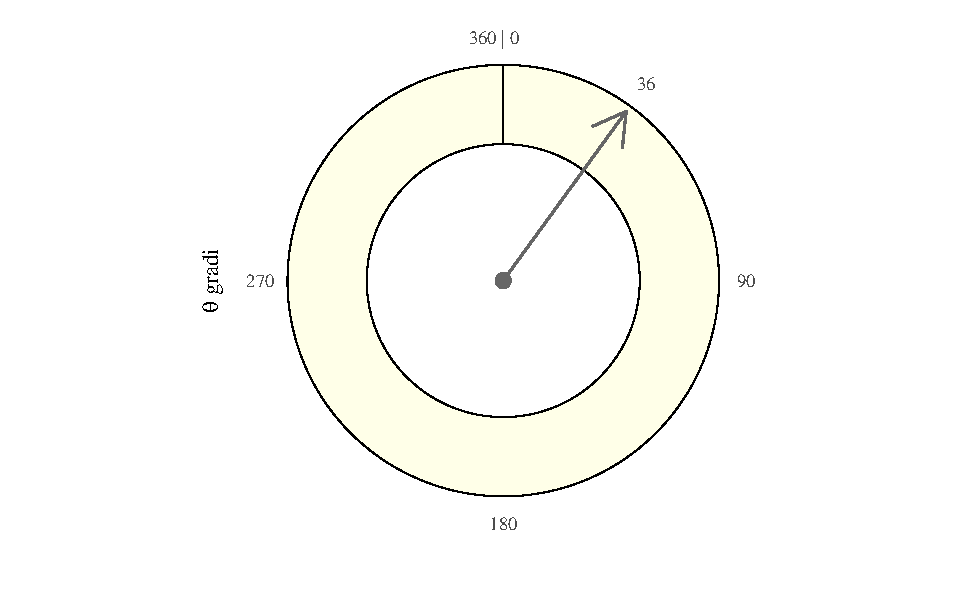
\includegraphics{ds4psy_files/figure-latex/unnamed-chunk-32-1} 

}

\caption{Probabilità del numero di successi in $N = 10$ prove bernoulliane indipendenti, ciascuna con una probabilità di successo di 0.90. Il risultato è una distribuzione $\Bin(y \mid 10, 0.9)$. Con solo dieci prove, la distribuzione è fortemente asimmetrica negativa.}\label{fig:unnamed-chunk-32}
\end{figure}

Ma se aumentiamo il numero di prove di un fattore di 100 a \emph{N} = 1000, senza modificare la probabilità di successo di 0.9, la distribuzione assume una forma campanulare quasi simmetrica. Dunque, de Moivre scoprì che, quando \emph{N} è grande, la funzione Normale (che introdurremo qui sotto), nonostante sia la densità di v.a. continue, fornisce una buona approssimazione alla funzione di massa di probabilità binomiale.

\begin{Shaded}
\begin{Highlighting}[]
\NormalTok{N }\OtherTok{\textless{}{-}} \DecValTok{1000}
\NormalTok{x }\OtherTok{\textless{}{-}} \DecValTok{0}\SpecialCharTok{:}\DecValTok{1000}
\NormalTok{y }\OtherTok{\textless{}{-}} \FunctionTok{dbinom}\NormalTok{(x, N, }\FloatTok{0.9}\NormalTok{)}
\NormalTok{binomial\_limit\_plot }\OtherTok{\textless{}{-}}
  \FunctionTok{tibble}\NormalTok{(}\AttributeTok{x =}\NormalTok{ x, }\AttributeTok{y =}\NormalTok{ y) }\SpecialCharTok{\%\textgreater{}\%}
  \FunctionTok{ggplot}\NormalTok{(}\FunctionTok{aes}\NormalTok{(}\AttributeTok{x =}\NormalTok{ x, }\AttributeTok{y =}\NormalTok{ y)) }\SpecialCharTok{+}
  \FunctionTok{geom\_bar}\NormalTok{(}\AttributeTok{stat =} \StringTok{"identity"}\NormalTok{, }\AttributeTok{color =} \StringTok{"black"}\NormalTok{, }\AttributeTok{size =} \FloatTok{0.2}\NormalTok{) }\SpecialCharTok{+}
  \FunctionTok{xlab}\NormalTok{(}\StringTok{"y"}\NormalTok{) }\SpecialCharTok{+}
  \FunctionTok{ylab}\NormalTok{(}\StringTok{"Binomial(y | 1000, 0.9)"}\NormalTok{) }\SpecialCharTok{+}
  \FunctionTok{xlim}\NormalTok{(}\DecValTok{850}\NormalTok{, }\DecValTok{950}\NormalTok{)}
\NormalTok{binomial\_limit\_plot}
\end{Highlighting}
\end{Shaded}

\begin{figure}[h]

{\centering 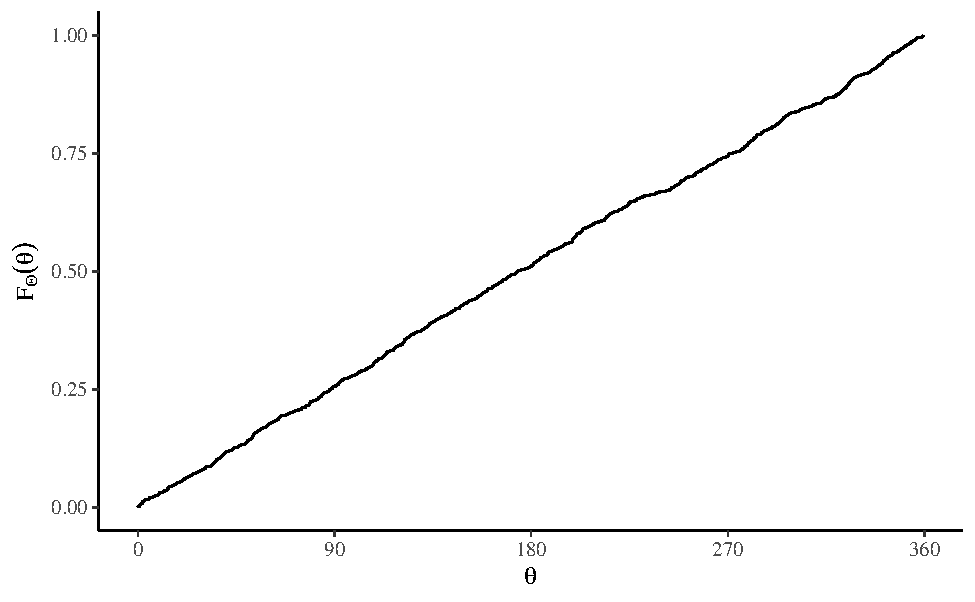
\includegraphics{ds4psy_files/figure-latex/unnamed-chunk-33-1} 

}

\caption{Probabilità del numero di successi in $N = 1000$ prove bernoulliane indipendenti, ciascuna con una probabilità di successo di 0.90. Il risultato è una distribuzione $\Bin(y \mid 1000, 0.9)$. Con mille prove, la distribuzione è quasi simmetrica a forma campanulare.}\label{fig:unnamed-chunk-33}
\end{figure}

La distribuzione Normale fu scoperta da Gauss nel 1809 e, storicamente, è intimamente legata al metodo dei minimi quadrati -- si veda l'Appendice \ref{gauss-normale}. Il Paragrafo successivo illustra come si possa giungere alla Normale mediante una simulazione.

\hypertarget{normal-random-walk}{%
\section{La Normale prodotta con una simulazione}\label{normal-random-walk}}

\citet{McElreath_rethinking} presenta un esempio che illustra come sia possibile giungere alla distribuzione Normale mediante una simulazione. Supponiamo che vi siano mille persone tutte allineate su una linea di partenza. Quando viene dato un segnale, ciascuna persona lancia una moneta e fa un passo in avanti oppure all'indietro a seconda che sia uscita testa o croce. Supponiamo che la lunghezza di ciascun passo vari da 0 a 1 metro. Ciascuna persona lancia una moneta 16 volte e dunque compie 16 passi.

Alla conclusione di queste passeggiate casuali (\emph{random walk}) non possiamo sapere con esattezza dove si troverà ciascuna persona, ma possiamo conoscere con certezza le caratteristiche della distribuzione delle mille distanze dall'origine. Per esempio, possiamo predire in maniera accurata la proporzione di persone che si sono spostate in avanti oppure all'indietro. Oppure, possiamo predire accuratamente la proporzione di persone che si troveranno ad una certa distanza dalla linea di partenza (es., a 1.5 m dall'origine).

Queste predizioni sono possibili perché tali distanze si distribuiscono secondo la legge Normale. È facile simulare questo processo usando \R. I risultati della simulazione sono riportati nella figura \ref{fig:rw-normal-4816}.

\begin{Shaded}
\begin{Highlighting}[]
\NormalTok{pos }\OtherTok{\textless{}{-}}
  \FunctionTok{replicate}\NormalTok{(}\DecValTok{100}\NormalTok{, }\FunctionTok{runif}\NormalTok{(}\DecValTok{16}\NormalTok{, }\SpecialCharTok{{-}}\DecValTok{1}\NormalTok{, }\DecValTok{1}\NormalTok{)) }\SpecialCharTok{\%\textgreater{}\%}
  \FunctionTok{as\_tibble}\NormalTok{() }\SpecialCharTok{\%\textgreater{}\%}
  \FunctionTok{rbind}\NormalTok{(}\DecValTok{0}\NormalTok{, .) }\SpecialCharTok{\%\textgreater{}\%}
  \FunctionTok{mutate}\NormalTok{(}\AttributeTok{step =} \DecValTok{0}\SpecialCharTok{:}\DecValTok{16}\NormalTok{) }\SpecialCharTok{\%\textgreater{}\%}
  \FunctionTok{gather}\NormalTok{(key, value, }\SpecialCharTok{{-}}\NormalTok{step) }\SpecialCharTok{\%\textgreater{}\%}
  \FunctionTok{mutate}\NormalTok{(}\AttributeTok{person =} \FunctionTok{rep}\NormalTok{(}\DecValTok{1}\SpecialCharTok{:}\DecValTok{100}\NormalTok{, }\AttributeTok{each =} \DecValTok{17}\NormalTok{)) }\SpecialCharTok{\%\textgreater{}\%}
  \FunctionTok{group\_by}\NormalTok{(person) }\SpecialCharTok{\%\textgreater{}\%}
  \FunctionTok{mutate}\NormalTok{(}\AttributeTok{position =} \FunctionTok{cumsum}\NormalTok{(value)) }\SpecialCharTok{\%\textgreater{}\%}
  \FunctionTok{ungroup}\NormalTok{()}

\FunctionTok{ggplot}\NormalTok{(}
  \AttributeTok{data =}\NormalTok{ pos,}
  \FunctionTok{aes}\NormalTok{(}\AttributeTok{x =}\NormalTok{ step, }\AttributeTok{y =}\NormalTok{ position, }\AttributeTok{group =}\NormalTok{ person)}
\NormalTok{) }\SpecialCharTok{+}
  \FunctionTok{geom\_vline}\NormalTok{(}\AttributeTok{xintercept =} \FunctionTok{c}\NormalTok{(}\DecValTok{4}\NormalTok{, }\DecValTok{8}\NormalTok{, }\DecValTok{16}\NormalTok{), }\AttributeTok{linetype =} \DecValTok{2}\NormalTok{) }\SpecialCharTok{+}
  \FunctionTok{geom\_line}\NormalTok{(}\FunctionTok{aes}\NormalTok{(}\AttributeTok{color =}\NormalTok{ person }\SpecialCharTok{\textless{}} \DecValTok{2}\NormalTok{, }\AttributeTok{alpha =}\NormalTok{ person }\SpecialCharTok{\textless{}} \DecValTok{2}\NormalTok{)) }\SpecialCharTok{+}
  \FunctionTok{scale\_color\_manual}\NormalTok{(}\AttributeTok{values =} \FunctionTok{c}\NormalTok{(}\StringTok{"gray"}\NormalTok{, }\StringTok{"black"}\NormalTok{)) }\SpecialCharTok{+}
  \FunctionTok{scale\_alpha\_manual}\NormalTok{(}\AttributeTok{values =} \FunctionTok{c}\NormalTok{(}\DecValTok{1} \SpecialCharTok{/} \DecValTok{5}\NormalTok{, }\DecValTok{1}\NormalTok{)) }\SpecialCharTok{+}
  \FunctionTok{scale\_x\_continuous}\NormalTok{(}
    \StringTok{"Numero di passi"}\NormalTok{,}
    \AttributeTok{breaks =} \FunctionTok{c}\NormalTok{(}\DecValTok{0}\NormalTok{, }\DecValTok{4}\NormalTok{, }\DecValTok{8}\NormalTok{, }\DecValTok{12}\NormalTok{, }\DecValTok{16}\NormalTok{)}
\NormalTok{  ) }\SpecialCharTok{+}
  \FunctionTok{labs}\NormalTok{(}\AttributeTok{y =} \StringTok{"Posizione"}\NormalTok{) }\SpecialCharTok{+}
  \FunctionTok{theme}\NormalTok{(}\AttributeTok{legend.position =} \StringTok{"none"}\NormalTok{)}
\end{Highlighting}
\end{Shaded}

\begin{figure}[h]

{\centering 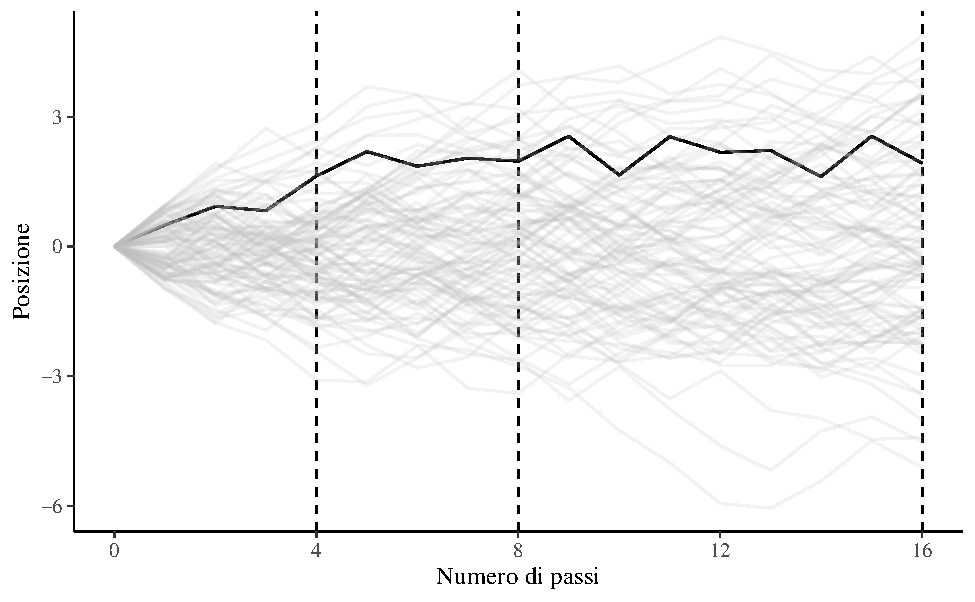
\includegraphics{ds4psy_files/figure-latex/rw-normal-4816-1} 

}

\caption{Passeggiata casuale di 4, 8 e 16 passi. La spezzata nera indica la media delle distanze dall'origine come funzione del numero di passi.}\label{fig:rw-normal-4816}
\end{figure}

Un kernel density plot delle distanze ottenute dopo 4, 8 e 16 passi è riportato nella figura \ref{fig:rw-normal-3panels}. Nel pannello di destra, al kernel density plot è stata sovrapposta una densità Normale di opportuni parametri (linea tratteggiata).

\begin{Shaded}
\begin{Highlighting}[]
\NormalTok{p1 }\OtherTok{\textless{}{-}}
\NormalTok{  pos }\SpecialCharTok{\%\textgreater{}\%}
  \FunctionTok{filter}\NormalTok{(step }\SpecialCharTok{==} \DecValTok{4}\NormalTok{) }\SpecialCharTok{\%\textgreater{}\%}
  \FunctionTok{ggplot}\NormalTok{(}\FunctionTok{aes}\NormalTok{(}\AttributeTok{x =}\NormalTok{ position)) }\SpecialCharTok{+}
  \FunctionTok{geom\_line}\NormalTok{(}\AttributeTok{stat =} \StringTok{"density"}\NormalTok{, }\AttributeTok{color =} \StringTok{"black"}\NormalTok{) }\SpecialCharTok{+}
  \FunctionTok{labs}\NormalTok{(}\AttributeTok{title =} \StringTok{"4 passi"}\NormalTok{)}

\NormalTok{p2 }\OtherTok{\textless{}{-}}
\NormalTok{  pos }\SpecialCharTok{\%\textgreater{}\%}
  \FunctionTok{filter}\NormalTok{(step }\SpecialCharTok{==} \DecValTok{8}\NormalTok{) }\SpecialCharTok{\%\textgreater{}\%}
  \FunctionTok{ggplot}\NormalTok{(}\FunctionTok{aes}\NormalTok{(}\AttributeTok{x =}\NormalTok{ position)) }\SpecialCharTok{+}
  \FunctionTok{geom\_density}\NormalTok{(}\AttributeTok{color =} \StringTok{"black"}\NormalTok{, }\AttributeTok{outline.type =} \StringTok{"full"}\NormalTok{) }\SpecialCharTok{+}
  \FunctionTok{labs}\NormalTok{(}\AttributeTok{title =} \StringTok{"8 passi"}\NormalTok{)}

\NormalTok{sd }\OtherTok{\textless{}{-}}
\NormalTok{  pos }\SpecialCharTok{\%\textgreater{}\%}
  \FunctionTok{filter}\NormalTok{(step }\SpecialCharTok{==} \DecValTok{16}\NormalTok{) }\SpecialCharTok{\%\textgreater{}\%}
  \FunctionTok{summarise}\NormalTok{(}\AttributeTok{sd =} \FunctionTok{sd}\NormalTok{(position)) }\SpecialCharTok{\%\textgreater{}\%}
  \FunctionTok{pull}\NormalTok{(sd)}

\NormalTok{p3 }\OtherTok{\textless{}{-}}
\NormalTok{  pos }\SpecialCharTok{\%\textgreater{}\%}
  \FunctionTok{filter}\NormalTok{(step }\SpecialCharTok{==} \DecValTok{16}\NormalTok{) }\SpecialCharTok{\%\textgreater{}\%}
  \FunctionTok{ggplot}\NormalTok{(}\FunctionTok{aes}\NormalTok{(}\AttributeTok{x =}\NormalTok{ position)) }\SpecialCharTok{+}
  \FunctionTok{stat\_function}\NormalTok{(}
    \AttributeTok{fun =}\NormalTok{ dnorm,}
    \AttributeTok{args =} \FunctionTok{list}\NormalTok{(}\AttributeTok{mean =} \DecValTok{0}\NormalTok{, }\AttributeTok{sd =}\NormalTok{ sd),}
    \AttributeTok{linetype =} \DecValTok{2}
\NormalTok{  ) }\SpecialCharTok{+}
  \FunctionTok{geom\_density}\NormalTok{(}\AttributeTok{color =} \StringTok{"black"}\NormalTok{, }\AttributeTok{alpha =} \DecValTok{1} \SpecialCharTok{/} \DecValTok{2}\NormalTok{) }\SpecialCharTok{+}
  \FunctionTok{labs}\NormalTok{(}
    \AttributeTok{title =} \StringTok{"16 passi"}\NormalTok{,}
    \AttributeTok{y =} \StringTok{"Densità"}
\NormalTok{  )}

\NormalTok{(p1 }\SpecialCharTok{|}\NormalTok{ p2 }\SpecialCharTok{|}\NormalTok{ p3) }\SpecialCharTok{\&} \FunctionTok{coord\_cartesian}\NormalTok{(}\AttributeTok{xlim =} \FunctionTok{c}\NormalTok{(}\SpecialCharTok{{-}}\DecValTok{6}\NormalTok{, }\DecValTok{6}\NormalTok{))}
\end{Highlighting}
\end{Shaded}

\begin{figure}[h]

{\centering 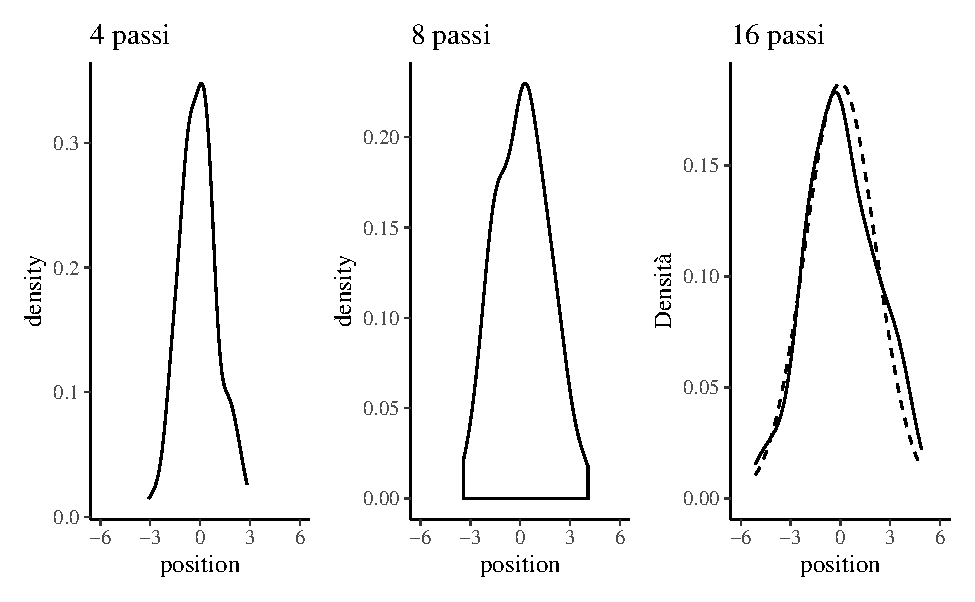
\includegraphics{ds4psy_files/figure-latex/rw-normal-3panels-1} 

}

\caption{Kernel density plot dei risultati della passeggiata casuale riportata nella figura precente, dopo 4, 8 e 16 passi. Nel pannello di destra, una densità Normale di opportuni parametri è sovrapposta all'istogramma lisciato.}\label{fig:rw-normal-3panels}
\end{figure}

Questa simulazione mostra che qualunque processo nel quale viene sommato un certo numero di valori casuali, tutti provenienti dalla medesima distribuzione, converge ad una distribuzione Normale. Non importa quale sia la forma della distribuzione di partenza: essa può essere uniforme, come nell'esempio presente, o di qualunque altro tipo. La forma della distribuzione da cui viene realizzato il campionamento determina la velocità della convergenza alla Normale. In alcuni casi la convergenza è lenta; in altri casi la convergenza è molto rapida (come nell'esempio presente).

Da un punto di vista formale, diciamo che una variabile casuale continua \(Y\) ha una distribuzione Normale se la sua densità è

\begin{equation}
f(y; \mu, \sigma) = {1 \over {\sigma\sqrt{2\pi} }} \exp \left\{-\frac{(y -  \mu)^2}{2 \sigma^2} \right\},
\label{eq:normal-formula}
\end{equation}

dove \(\mu \in \mathbb{R}\) e \(\sigma > 0\) sono i parametri della distribuzione.

La densità normale è unimodale e simmetrica con una caratteristica forma a campana e con il punto di massima densità in corrispondenza di \(\mu\).

Il significato dei parametri \(\mu\) e \(\sigma\) che appaiono nella \eqref{eq:normal-formula} viene chiarito dalla dimostrazione che

\begin{equation}
\E(X) = \mu, \qquad \Var(X) = \sigma^2.
\end{equation}

La rappresentazione grafica di quattro densità Normali tutte con media 0 e con deviazioni standard 0.25, 0.5, 1 e 2 è fornita nella figura \ref{fig:gaussian-plot-demo}.

\begin{figure}[h]

{\centering 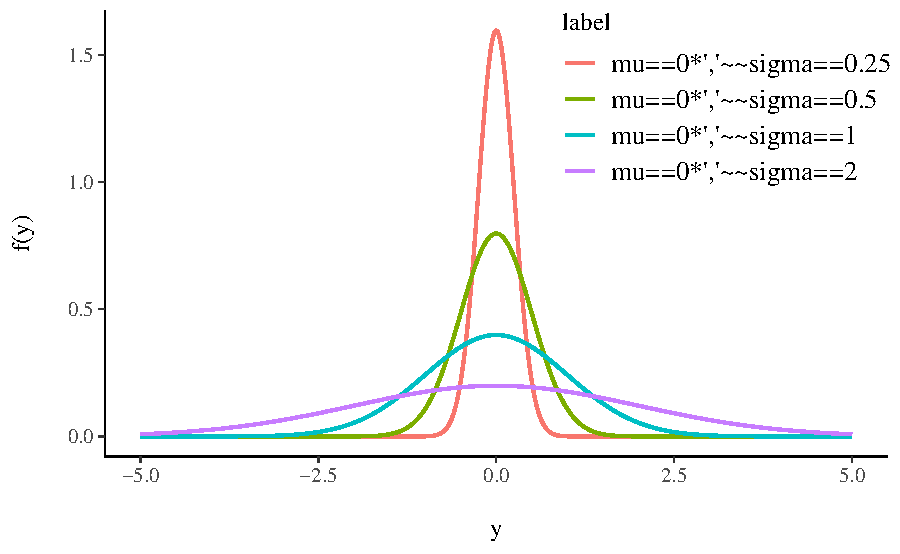
\includegraphics{ds4psy_files/figure-latex/gaussian-plot-demo-1} 

}

\caption{Alcune distribuzioni Normali.}\label{fig:gaussian-plot-demo}
\end{figure}

\hypertarget{concentrazione}{%
\subsection{Concentrazione}\label{concentrazione}}

È istruttivo osservare il grado di concentrazione della distribuzione Normale attorno alla media:

\begin{align}
P(\mu - \sigma < X < \mu + \sigma) &= P (-1 < Z < 1) \simeq 0.683, \notag\\
P(\mu - 2\sigma < X < \mu + 2\sigma) &= P (-2 < Z < 2) \simeq 0.956, \notag\\
P(\mu - 3\sigma < X < \mu + 3\sigma) &= P (-3 < Z < 3) \simeq 0.997. \notag
\end{align}

\noindent Si noti come un dato la cui distanza dalla media è superiore a 3 volte la deviazione standard presenti un carattere di eccezionalità perché meno del 0.3\% dei dati della distribuzione Normale presentano questa caratteristica.

Per indicare la distribuzione Normale si usa la notazione \(\mathcal{N}(\mu, \sigma)\).

\hypertarget{funzione-di-ripartizione-1}{%
\subsection{Funzione di ripartizione}\label{funzione-di-ripartizione-1}}

Il valore della funzione di ripartizione di \(Y\) nel punto \(y\) è l'area sottesa alla curva di densità \(f(y)\) nella semiretta \((-\infty, y]\). Non esiste alcuna funzione elementare per la funzione di ripartizione

\begin{equation}
F(y) = \int_{-\infty}^y {1 \over {\sigma\sqrt{2\pi} }} \exp \left\{-\frac{(y - \mu)^2}{2\sigma^2} \right\} dy, 
\end{equation}

pertanto le probabilità \(P(Y < y)\) vengono calcolate mediante integrazione numerica approssimata. I valori della funzione di ripartizione di una variabile casuale Normale sono dunque forniti da un software.

\begin{exercise}

Usiamo \R per calcolare la funzione di ripartizione della Normale. La funzione \texttt{pnorm(q,\ mean,\ sd)} restituisce la funzione di ripartizione della Normale con media \texttt{mean} e deviazione standard \texttt{sd}, ovvero l'area sottesa alla funzione di densità di una Normale con media \texttt{mean} e deviazione standard \texttt{sd} nell'intervallo \([-\infty, q]\).

Per esempio, in precedenza abbiamo detto che il 68\% circa dell'area sottesa ad una Normale è compresa nell'intervallo \(\mu \pm \sigma\). Verifichiamo per la distribuzione del QI \(\sim \mathcal{N}(\mu = 100, \sigma = 15)\):

\begin{Shaded}
\begin{Highlighting}[]
\FunctionTok{pnorm}\NormalTok{(}\DecValTok{100}\SpecialCharTok{+}\DecValTok{15}\NormalTok{, }\DecValTok{100}\NormalTok{, }\DecValTok{15}\NormalTok{) }\SpecialCharTok{{-}} \FunctionTok{pnorm}\NormalTok{(}\DecValTok{100{-}15}\NormalTok{, }\DecValTok{100}\NormalTok{, }\DecValTok{15}\NormalTok{)}
\CommentTok{\#\textgreater{} [1] 0.6827}
\end{Highlighting}
\end{Shaded}

Il 95\% dell'area è compresa nell'intervallo \(\mu \pm 1.96 \cdot\sigma\):

\begin{Shaded}
\begin{Highlighting}[]
\FunctionTok{pnorm}\NormalTok{(}\DecValTok{100} \SpecialCharTok{+} \FloatTok{1.96} \SpecialCharTok{*} \DecValTok{15}\NormalTok{, }\DecValTok{100}\NormalTok{, }\DecValTok{15}\NormalTok{) }\SpecialCharTok{{-}} \FunctionTok{pnorm}\NormalTok{(}\DecValTok{100} \SpecialCharTok{{-}} \FloatTok{1.96} \SpecialCharTok{*} \DecValTok{15}\NormalTok{, }\DecValTok{100}\NormalTok{, }\DecValTok{15}\NormalTok{)}
\CommentTok{\#\textgreater{} [1] 0.95}
\end{Highlighting}
\end{Shaded}

Quasi tutta la distribuzione è compresa nell'intervallo \(\mu \pm 3 \cdot\sigma\):

\begin{Shaded}
\begin{Highlighting}[]
\FunctionTok{pnorm}\NormalTok{(}\DecValTok{100} \SpecialCharTok{+} \DecValTok{3} \SpecialCharTok{*} \DecValTok{15}\NormalTok{, }\DecValTok{100}\NormalTok{, }\DecValTok{15}\NormalTok{) }\SpecialCharTok{{-}} \FunctionTok{pnorm}\NormalTok{(}\DecValTok{100} \SpecialCharTok{{-}} \DecValTok{3} \SpecialCharTok{*} \DecValTok{15}\NormalTok{, }\DecValTok{100}\NormalTok{, }\DecValTok{15}\NormalTok{)}
\CommentTok{\#\textgreater{} [1] 0.9973}
\end{Highlighting}
\end{Shaded}

\end{exercise}

\hypertarget{distribuzione-normale-standard}{%
\subsection{Distribuzione Normale standard}\label{distribuzione-normale-standard}}

La distribuzione Normale di parametri \(\mu = 0\) e \(\sigma = 1\) viene detta \emph{distribuzione Normale standard}. La famiglia Normale è l'insieme avente come elementi tutte le distribuzioni Normali con parametri \(\mu\) e \(\sigma\) diversi. Tutte le distribuzioni Normali si ottengono dalla Normale standard mediante una trasformazione lineare: se \(Y \sim \mathcal{N}(\mu_Y, \sigma_Y)\) allora

\begin{equation}
X = a + b Y \sim \mathcal{N}(\mu_X = a+b \mu_Y, \sigma_X = \left|b\right|\sigma_Y).
\end{equation}

L'area sottesa alla curva di densità di \(\mathcal{N}(\mu, \sigma)\) nella semiretta \((-\infty, y]\) è uguale all'area sottesa alla densità Normale standard nella semiretta \((-\infty, z]\), in cui \(z = (y -\mu_Y )/\sigma_Y\) è il punteggio standard di \(Y\). Per la simmetria della distribuzione, l'area sottesa nella semiretta \([1, \infty)\) è uguale all'area sottesa nella semiretta \((-\infty, 1]\) e quest'ultima coincide con \(F(-1)\). Analogamente, l'area sottesa nell'intervallo \([y_a, y_b]\), con \(y_a < y_b\), è pari a \(F(z_b) - F(z_a)\), dove \(z_a\) e \(z_b\) sono i punteggi standard di \(y_a\) e \(y_b\).

Si ha anche il problema inverso rispetto a quello del calcolo delle aree: dato un numero \(0 \leq p \leq 1\), il problema è quello di determinare un numero \(z \in \mathbb{R}\) tale che \(P(Z < z) = p\). Il valore \(z\) cercato è detto \emph{quantile} di ordine \(p\) della Normale standard e può essere trovato mediante un software.

\begin{exercise}
Supponiamo che l'altezza degli individui adulti segua la distribuzione Normale di media \(\mu = 1.7\) m e deviazione standard \(\sigma = 0.1\) m. Vogliamo sapere la proporzione di individui adulti con un'altezza compresa tra \(1.7\) e \(1.8\) m.

Il problema ci chiede di trovare l'area sottesa alla distribuzione \(\mathcal{N}(\mu = 1.7, \sigma = 0.1)\) nell'intervallo \([1.7, 1.8]\):

\begin{Shaded}
\begin{Highlighting}[]
\NormalTok{df }\OtherTok{\textless{}{-}} \FunctionTok{tibble}\NormalTok{(}\AttributeTok{x =} \FunctionTok{seq}\NormalTok{(}\FloatTok{1.4}\NormalTok{, }\FloatTok{2.0}\NormalTok{, }\AttributeTok{length.out =} \DecValTok{100}\NormalTok{)) }\SpecialCharTok{\%\textgreater{}\%}
  \FunctionTok{mutate}\NormalTok{(}\AttributeTok{y =} \FunctionTok{dnorm}\NormalTok{(x, }\AttributeTok{mean =} \FloatTok{1.7}\NormalTok{, }\AttributeTok{sd =} \FloatTok{0.1}\NormalTok{))}

\FunctionTok{ggplot}\NormalTok{(df, }\FunctionTok{aes}\NormalTok{(x, y)) }\SpecialCharTok{+}
  \FunctionTok{geom\_area}\NormalTok{(}\AttributeTok{fill =} \StringTok{"sky blue"}\NormalTok{) }\SpecialCharTok{+}
  \FunctionTok{gghighlight}\NormalTok{(x }\SpecialCharTok{\textless{}} \FloatTok{1.8} \SpecialCharTok{\&}\NormalTok{ x }\SpecialCharTok{\textgreater{}} \FloatTok{1.7}\NormalTok{) }\SpecialCharTok{+}
  \FunctionTok{labs}\NormalTok{(}
    \AttributeTok{x =} \StringTok{"Altezza"}\NormalTok{,}
    \AttributeTok{y =} \StringTok{"Densità"}
\NormalTok{  )}
\end{Highlighting}
\end{Shaded}

\begin{center}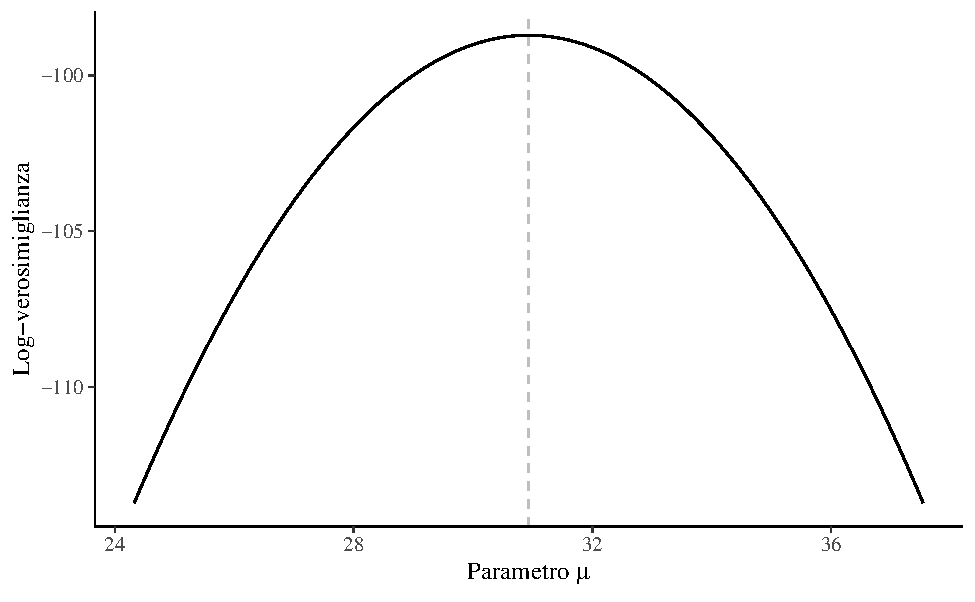
\includegraphics{ds4psy_files/figure-latex/unnamed-chunk-37-1} \end{center}

\noindent La risposta si trova utilizzando la funzione di ripartizione \(F(X)\) della legge \(\mathcal{N}(1.7, 0.1)\) in corrispondenza dei due valori forniti dal problema: \(F(X = 1.8) - F(X = 1.7)\). Utilizzando la seguente istruzione

\begin{Shaded}
\begin{Highlighting}[]
\FunctionTok{pnorm}\NormalTok{(}\FloatTok{1.8}\NormalTok{, }\FloatTok{1.7}\NormalTok{, }\FloatTok{0.1}\NormalTok{) }\SpecialCharTok{{-}} \FunctionTok{pnorm}\NormalTok{(}\FloatTok{1.7}\NormalTok{, }\FloatTok{1.7}\NormalTok{, }\FloatTok{0.1}\NormalTok{)}
\CommentTok{\#\textgreater{} [1] 0.3413}
\end{Highlighting}
\end{Shaded}

otteniamo il \(31.43\%\).

In maniera equivalente, possiamo standardizzare i valori che delimitano l'intervallo considerato e utilizzare la funzione di ripartizione della normale standardizzata. I limiti inferiore e superiore dell'intervallo sono

\[
z_{\text{inf}} = \frac{1.7 - 1.7}{0.1} = 0, \quad z_{\text{sup}} = \frac{1.8 - 1.7}{0.1} = 1.0,
\]

quindi otteniamo

\begin{Shaded}
\begin{Highlighting}[]
\FunctionTok{pnorm}\NormalTok{(}\FloatTok{1.0}\NormalTok{, }\DecValTok{0}\NormalTok{, }\DecValTok{1}\NormalTok{) }\SpecialCharTok{{-}} \FunctionTok{pnorm}\NormalTok{(}\DecValTok{0}\NormalTok{, }\DecValTok{0}\NormalTok{, }\DecValTok{1}\NormalTok{)}
\CommentTok{\#\textgreater{} [1] 0.3413}
\end{Highlighting}
\end{Shaded}

Il modo più semplice per risolvere questo problema resta comunque quello di rendersi conto che la probabilità richiesta non è altro che la metà dell'area sottesa dalle distribuzioni Normali nell'intervallo \([\mu - \sigma, \mu + \sigma]\), ovvero \(0.683/2\).
\end{exercise}

\hypertarget{funzione-di-ripartizione-della-normale-standard-e-funzione-logistica}{%
\subsubsection{Funzione di ripartizione della normale standard e funzione logistica}\label{funzione-di-ripartizione-della-normale-standard-e-funzione-logistica}}

Si noti che la funzione logistica (in blu), pur essendo del tutto diversa dalla Normale dal punto di vista formale, assomiglia molto alla Normale standard quando le due cdf hanno la stessa varianza.

\begin{Shaded}
\begin{Highlighting}[]
\FunctionTok{tibble}\NormalTok{(}\AttributeTok{x =} \FunctionTok{c}\NormalTok{(}\SpecialCharTok{{-}}\DecValTok{3}\NormalTok{, }\DecValTok{3}\NormalTok{)) }\SpecialCharTok{\%\textgreater{}\%}
  \FunctionTok{ggplot}\NormalTok{(}\FunctionTok{aes}\NormalTok{(}\AttributeTok{x =}\NormalTok{ x)) }\SpecialCharTok{+}
  \FunctionTok{stat\_function}\NormalTok{(}\AttributeTok{fun =}\NormalTok{ pnorm) }\SpecialCharTok{+}
  \FunctionTok{stat\_function}\NormalTok{(}
    \AttributeTok{fun =}\NormalTok{ plogis,}
    \AttributeTok{args =} \FunctionTok{list}\NormalTok{(}\AttributeTok{scale =} \FloatTok{0.56}\NormalTok{)}
\NormalTok{  )}
\end{Highlighting}
\end{Shaded}

\begin{center}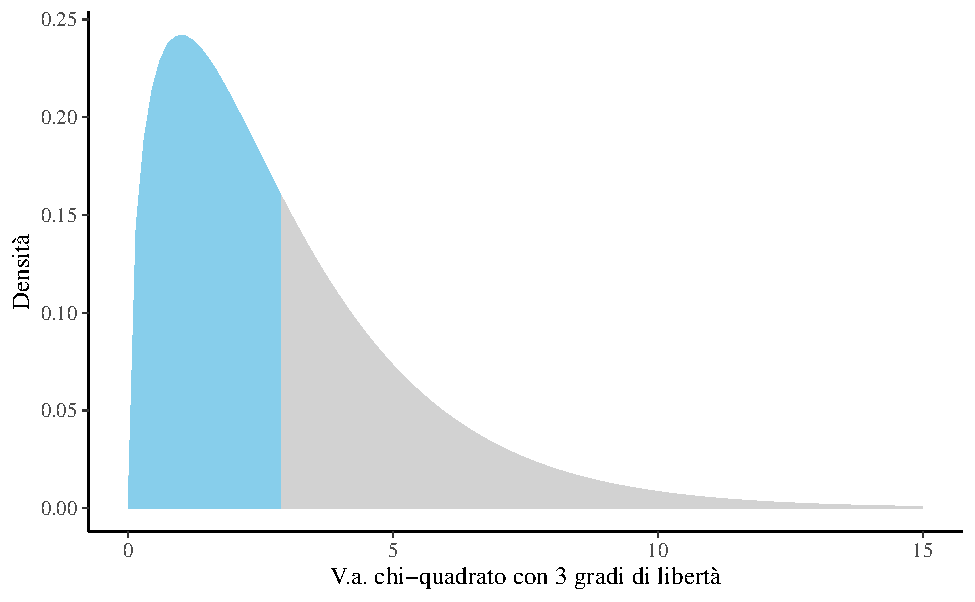
\includegraphics{ds4psy_files/figure-latex/unnamed-chunk-40-1} \end{center}

\hypertarget{teorema-del-limite-centrale}{%
\section{Teorema del limite centrale}\label{teorema-del-limite-centrale}}

Laplace dimostrò il teorema del limite centrale (TLC) nel 1812. Il TLC ci dice che se prendiamo una sequenza di variabili casuali indipendenti e le sommiamo, tale somma tende a distribuirisi come una Normale. Il TLC specifica inoltre, sulla base dei valori attesi e delle varianze delle v.c. che vengono sommate, quali saranno i parametri della distribuzione Normale così ottenuta.

\begin{theorem}
Si supponga che \(Y = Y_1, Y_2, \ldots, Y_N\) sia una sequenza di v.a. i.i.d. con \(\E(Y_n) = \mu\) e \(\SD(Y_n) = \sigma\). Si definisca una nuova v.c. come la media di \(Y\):

\[
Z = \frac{1}{N} \sum_{n=1}^N Y_n.
\]

Con \(N \rightarrow \infty\), \(Z\) tenderà ad una Normale con lo stesso valore atteso di \(Y_n\) e una deviazione standard che sarà più piccola della deviazione standard originaria di un fattore pari a \(\sqrt{\frac{1}{\sqrt{N}}}\):

\begin{equation}
p_Z(z) \rightarrow \mathcal{N}\left(z \ \Bigg| \ \mu, \, \frac{1}{\sqrt{N}} \cdot \sigma \right).
\end{equation}
\end{theorem}

Il TLC può essere generalizzato a variabili che non hanno la stessa distribuzione purché siano indipendenti e abbiano aspettative e varianze finite.

Molti fenomeni naturali, come l'altezza dell'uomo adulto di entrambi i sessi, sono il risultato di una serie di effetti additivi relativamente piccoli, la cui combinazione porta alla normalità, indipendentemente da come gli effetti additivi sono distribuiti. In pratica, questo è il motivo per cui la distribuzione normale ha senso come rappresentazione di molti fenomeni naturali.

\hypertarget{distribuzione-chi-quadrato}{%
\section{Distribuzione Chi-quadrato}\label{distribuzione-chi-quadrato}}

Dalla Normale deriva la distribuzione \(\chi^2\). La distribuzione \(\chi^2_{~k}\) con \(k\) gradi di libertà descrive la variabile casuale

\[
Z_1^2 + Z_2^2 + \dots + Z_k^2,
\]

dove \(Z_1, Z_2, \dots, Z_k\) sono variabili casuali i.i.d. con distribuzione Normale standard \(\mathcal{N}(0, 1)\). La variabile casuale chi-quadrato dipende dal parametro intero positivo \(\nu = k\) che ne identifica il numero di gradi di libertà. La densità di probabilità di \(\chi^2_{~\nu}\) è

\[
f(x) = C_{\nu} x^{\nu/2-1} \exp (-x/2), \qquad \text{se } x > 0,
\]

dove \(C_{\nu}\) è una costante positiva.

La figura \ref{fig:alcune-chi-quadrato} mostra alcune distribuzioni Chi-quadrato variando il parametro \(\nu\).

\begin{figure}[h]

{\centering 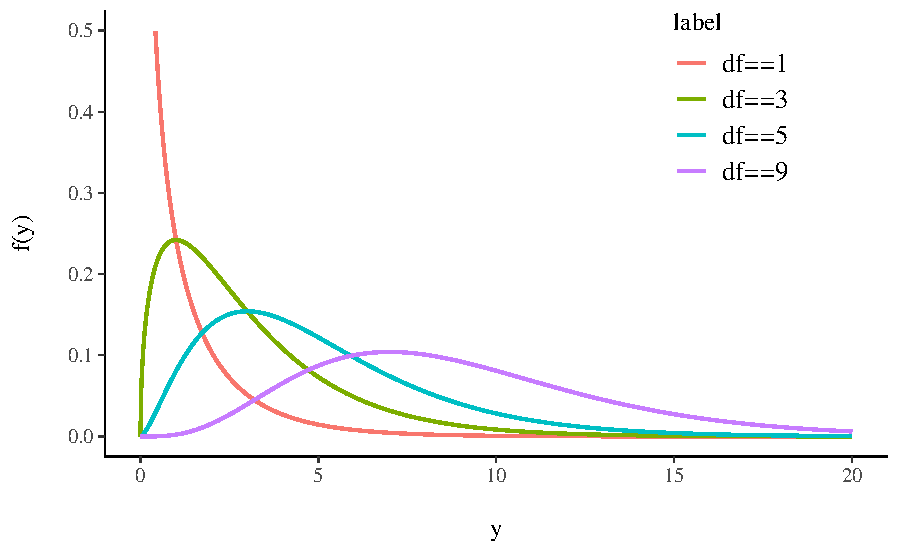
\includegraphics{ds4psy_files/figure-latex/alcune-chi-quadrato-1} 

}

\caption{Alcune distribuzioni Chi-quadrato.}\label{fig:alcune-chi-quadrato}
\end{figure}

\hypertarget{proprietuxe0-1}{%
\subsection{Proprietà}\label{proprietuxe0-1}}

\begin{itemize}
\item
  La distribuzione di densità \(\chi^2_{~\nu}\) è asimmetrica.
\item
  Il valore atteso di una variabile \(\chi^2_{~\nu}\) è uguale a \(\nu\).
\item
  La varianza di una variabile \(\chi^2_{~\nu}\) è uguale a \(2\nu\).
\item
  Per \(k \rightarrow \infty\), la \(\chi^2_{~\nu} \rightarrow \mathcal{N}\).
\item
  Se \(X\) e \(Y\) sono due variabili casuali chi-quadrato indipendenti con \(\nu_1\) e \(\nu_2\) gradi di libertà, ne segue che \(X + Y \sim \chi^2_m\), con \(m = \nu_1 + \nu_2\). Tale principio si estende a qualunque numero finito di variabili casuali chi-quadrato indipendenti.
\end{itemize}

\begin{exercise}

Usiamo \(\R\) per disegnare la densità chi-quadrato con 3 gradi di libertà dividendo l'area sottesa alla curva di densità in due parti uguali.

\begin{Shaded}
\begin{Highlighting}[]
\NormalTok{df }\OtherTok{\textless{}{-}} \FunctionTok{tibble}\NormalTok{(}\AttributeTok{x =} \FunctionTok{seq}\NormalTok{(}\DecValTok{0}\NormalTok{, }\FloatTok{15.0}\NormalTok{, }\AttributeTok{length.out =} \DecValTok{100}\NormalTok{)) }\SpecialCharTok{\%\textgreater{}\%}
  \FunctionTok{mutate}\NormalTok{(}\AttributeTok{y =} \FunctionTok{dchisq}\NormalTok{(x, }\DecValTok{3}\NormalTok{))}

\FunctionTok{ggplot}\NormalTok{(df, }\FunctionTok{aes}\NormalTok{(x, y)) }\SpecialCharTok{+}
  \FunctionTok{geom\_area}\NormalTok{(}\AttributeTok{fill =} \StringTok{"sky blue"}\NormalTok{) }\SpecialCharTok{+}
  \FunctionTok{gghighlight}\NormalTok{(x }\SpecialCharTok{\textless{}} \DecValTok{3}\NormalTok{) }\SpecialCharTok{+}
  \FunctionTok{labs}\NormalTok{(}
    \AttributeTok{x =} \StringTok{"V.a. chi{-}quadrato con 3 gradi di libertà"}\NormalTok{,}
    \AttributeTok{y =} \StringTok{"Densità"}
\NormalTok{  )}
\end{Highlighting}
\end{Shaded}

\begin{center}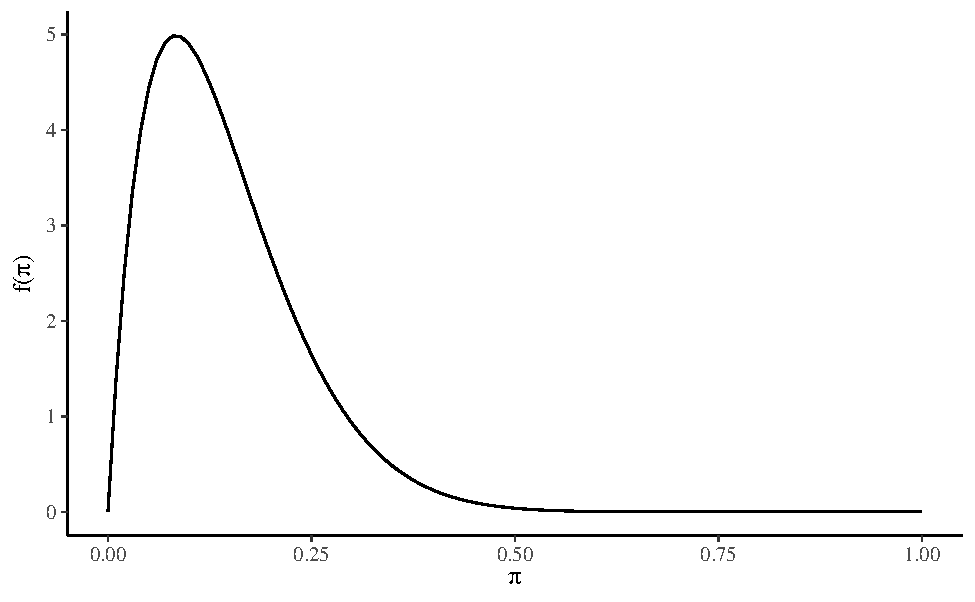
\includegraphics{ds4psy_files/figure-latex/unnamed-chunk-41-1} \end{center}

\end{exercise}

\hypertarget{distribuzione-t-di-student}{%
\section{\texorpdfstring{Distribuzione \(t\) di Student}{Distribuzione t di Student}}\label{distribuzione-t-di-student}}

Dalle distribuzioni Normale e Chi quadrato deriva un'altra distribuzione molto nota, la \(t\) di Student. Se \(Z \sim \mathcal{N}\) e \(W \sim \chi^2_{~\nu}\) sono due variabili casuali indipendenti, allora il rapporto

\begin{equation}
T = \frac{Z}{\Big( \frac{W}{\nu}\Big)^{\frac{1}{2}}}
\end{equation}

definisce la distribuzione \(t\) di Student con \(\nu\) gradi di libertà. Si usa scrivere \(T \sim t_{\nu}\). L'andamento della distribuzione \(t\) di Student è simile a quello della distribuzione Normale, ma ha una maggiore dispersione (ha le code più pesanti di una Normale, ovvero ha una varianza maggiore di 1).

La figura \ref{fig:alcune-t-student} mostra alcune distribuzioni \(t\) di Student variando il parametro \(\nu\).

\begin{figure}[h]

{\centering 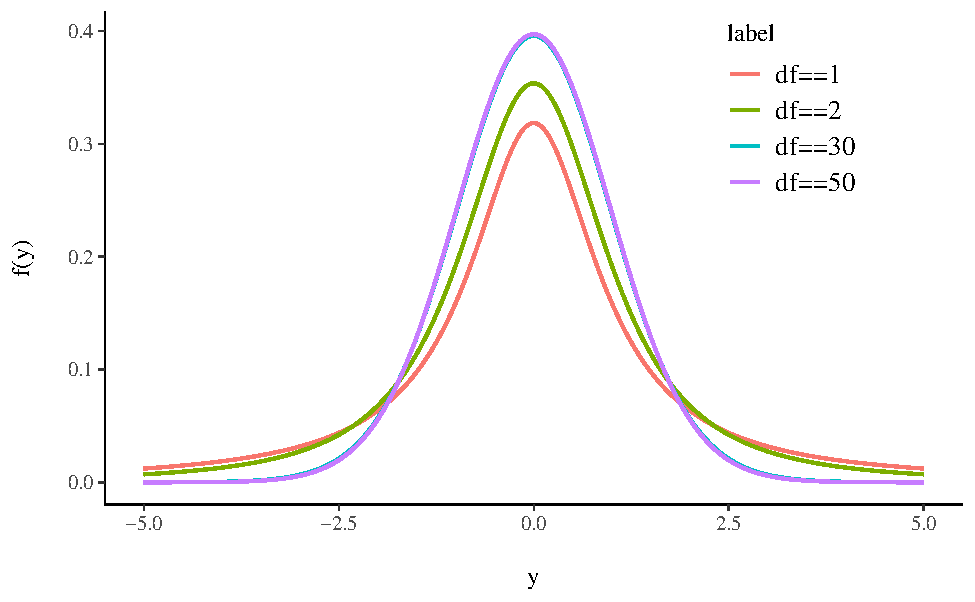
\includegraphics{ds4psy_files/figure-latex/alcune-t-student-1} 

}

\caption{Alcune distribuzioni $t$ di Student.}\label{fig:alcune-t-student}
\end{figure}

\hypertarget{proprietuxe0-2}{%
\subsection{Proprietà}\label{proprietuxe0-2}}

La variabile casuale \(t\) di Student soddisfa le seguenti proprietà:

\begin{enumerate}
\def\labelenumi{\arabic{enumi}.}
\item
  Per \(\nu \rightarrow \infty\), \(t_{\nu}\) tende alla normale standard \(\mathcal{N}(0, 1)\).
\item
  La densità della \(t_{\nu}\) è una funzione simmetrica con valore atteso nullo.
\item
  Per \(\nu > 2\), la varianza della \(t_{\nu}\) vale \(\nu/(\nu - 2)\); pertanto è sempre maggiore di 1 e tende a 1 per \(\nu \rightarrow \infty\).
\end{enumerate}

\hypertarget{funzione-beta-di-eulero}{%
\section{Funzione beta di Eulero}\label{funzione-beta-di-eulero}}

La funzione beta di Eulero è una funzione matematica, \emph{non} una densità di probabilità. La menzioniamo qui perché viene utilizzata nella distribuzione Beta. La funzione beta si può scrivere in molti modi diversi; per i nostri scopi la scriveremo così:

\begin{equation}
B(\alpha, \beta) = \frac{\Gamma(\alpha)\Gamma(\beta)}{\Gamma(\alpha + \beta)}\,,
\end{equation}

dove \(\Gamma(x)\) è la funzione Gamma, ovvero il fattoriale discendente, cioè \begin{equation}
x(x-1)(x-2)\ldots (x-n+1)\notag\,.
\end{equation}

\hypertarget{distribuzione-beta}{%
\section{Distribuzione Beta}\label{distribuzione-beta}}

Una distribuzione che viene usata per modellare percentuali e proporzioni è la distribuzione Beta in quanto è definita sull'intervallo \((0; 1)\) -- ma non include i valori 0 o 1. La distribuzione Beta è una distribuzione estremamente flessibile e può assumere molti tipi di forme diverse (un'illustrazione è fornita dalla seguente \href{https://en.wikipedia.org/wiki/File:PDF_of_the_Beta_distribution.gif}{GIF animata}). Una definizione formale è la seguente.

\begin{definition}
Sia \(\pi\) una variabile casuale che può assumere qualsiasi valore compreso tra 0 e 1, cioè \(\pi \in [0, 1]\). Diremo che \(\pi\) segue la distribuzione Beta di parametri \(\alpha\) e \(\beta\), \(\pi \sim \text{Beta}(\alpha, \beta)\), se la sua densità è

\begin{align}
\text{Beta}(\pi \mid \alpha, \beta) &= \frac{1}{B(\alpha, \beta)}\pi^{\alpha-1} (1-\pi)^{\beta-1}\notag\\ 
&=  \frac{\Gamma(\alpha+ \beta)}{\Gamma(\alpha)\Gamma(\beta)}\pi^{\alpha-1} (1-\pi)^{\beta-1} \quad \text{per } \pi \in [0, 1]\,,
\label{eq:beta-distr-formula}
\end{align}

laddove \(B(\alpha, \beta)\) è la funzione beta.
\end{definition}

I termini \(\alpha\) e \(\beta\) sono i parametri della distribuzione Beta e devono essere entrambi positivi. Tali parametri possono essere interpretati come l'espressione delle nostre credenze a priori relative ad una sequenza di prove Bernoulliane Il parametro \(\alpha\) rappresenta il numero di ``successi'' e il parametro \(\beta\) il numero di ``insuccessi'':

\begin{equation}
\frac{\text{Numero di successi}}{\text{Numero di successi} + \text{Numero di insuccessi}} = \frac{\alpha}{\alpha + \beta}\notag\,.
\end{equation}

Il rapporto \(\frac{1}{B(\alpha, \beta)} = \frac{\Gamma(\alpha+b)}{\Gamma(\alpha)\Gamma(\beta)}\) è una costante di normalizzazione:

\begin{equation}
\int_0^1 \pi^{\alpha-1} (1-\pi)^{\beta-1} = \frac{\Gamma(\alpha+b)}{\Gamma(\alpha)\Gamma(\beta)}\,.
\end{equation}

Il valore atteso, la moda e la varianza di una distribuzione Beta sono dati dalle seguenti equazioni:

\begin{equation}
\E(\pi) = \frac{\alpha}{\alpha+\beta}\,,
\label{eq:beta-mean}
\end{equation}

\begin{equation}
\Mo(\pi) = \frac{\alpha-1}{\alpha+\beta-2}\,,
\label{eq:beta-mode}
\end{equation}

\begin{equation}
\Var(\pi) = \frac{\alpha \beta}{(\alpha+\beta)^2 (\alpha+\beta+1)}\,.
\label{eq:beta-var}
\end{equation}

\begin{remark}

Attenzione alle parole: in questo contesto, il termine ``beta'' viene utilizzato con tre significati diversi:

\begin{itemize}
\item
  la distribuzione di densità Beta,
\item
  la funzione matematica beta,
\item
  il parametro \(\beta\).
\end{itemize}

\end{remark}

Al variare di \(\alpha\) e \(\beta\) si ottengono molte distribuzioni di forma diversa; per \(\alpha = \beta = 1\) si ha la densità uniforme. Vari esempi di distribuzioni Beta sono mostrati nella figura \ref{fig:some-beta-distr}.

\begin{figure}[h]

{\centering 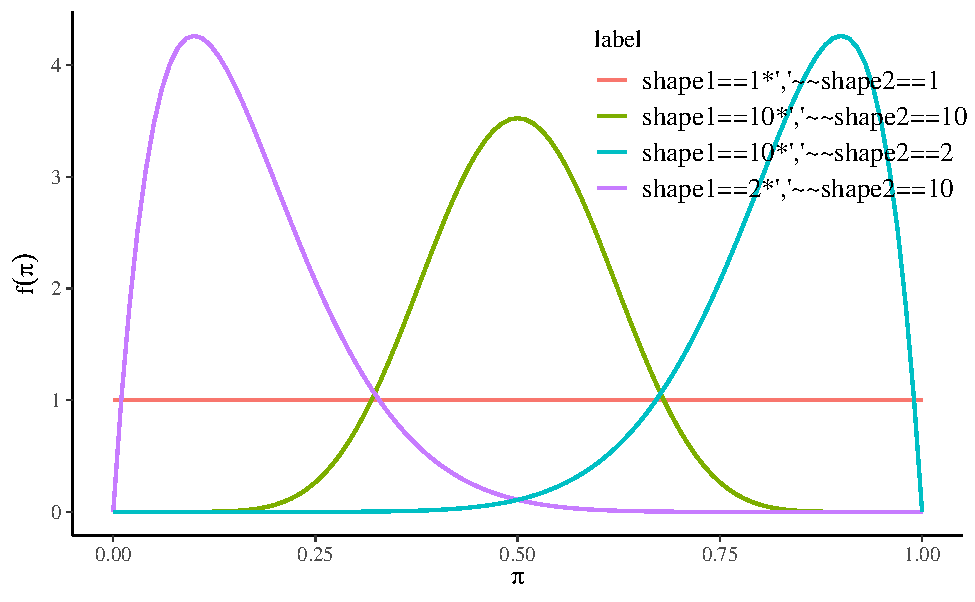
\includegraphics{ds4psy_files/figure-latex/some-beta-distr-1} 

}

\caption{Alcune distribuzioni Beta.}\label{fig:some-beta-distr}
\end{figure}

Si può ottenere una rappresentazione grafica della distribuzione \(\mbox{Beta}(\pi \mid \alpha, \beta)\) con la funzione \texttt{plot\_beta()} del pacchetto \texttt{bayesrules}. Per esempio:

\begin{Shaded}
\begin{Highlighting}[]
\NormalTok{bayesrules}\SpecialCharTok{::}\FunctionTok{plot\_beta}\NormalTok{(}\AttributeTok{alpha =} \DecValTok{2}\NormalTok{, }\AttributeTok{beta =} \DecValTok{12}\NormalTok{)}
\end{Highlighting}
\end{Shaded}

\begin{center}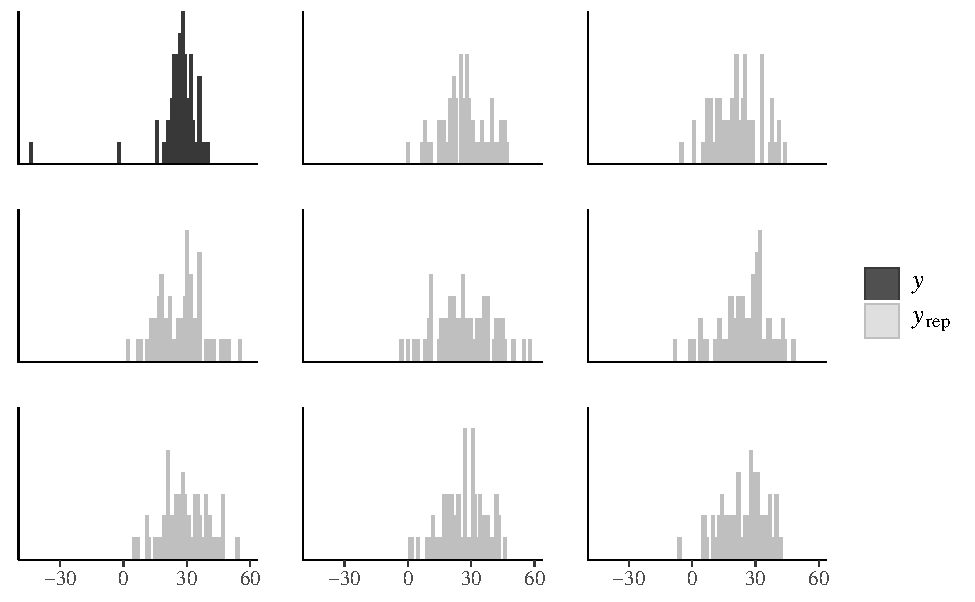
\includegraphics{ds4psy_files/figure-latex/unnamed-chunk-42-1} \end{center}

La funzione \texttt{bayesrules::summarize\_beta()} ci restituisce la media, moda e varianza della distribuzione Beta. Per esempio:

\begin{Shaded}
\begin{Highlighting}[]
\NormalTok{bayesrules}\SpecialCharTok{::}\FunctionTok{summarize\_beta}\NormalTok{(}\AttributeTok{alpha =} \DecValTok{2}\NormalTok{, }\AttributeTok{beta =} \DecValTok{12}\NormalTok{)}
\CommentTok{\#\textgreater{}     mean    mode      var      sd}
\CommentTok{\#\textgreater{} 1 0.1429 0.08333 0.008163 0.09035}
\end{Highlighting}
\end{Shaded}

\begin{exercise}
Nel disturbo depressivo la recidiva è definita come la comparsa di un nuovo episodio depressivo che si manifesta dopo un prolungato periodo di recupero (6-12 mesi) con stato di eutimia (umore relativamente normale). Supponiamo che una serie di studi mostri una comparsa di recidiva in una proporzione che va dal 20\% al 60\% dei casi, con una media del 40\% \citep[per una recente discussione, si veda][]{nuggerud2020analysis}. Sulla base di queste ipotetiche informazioni, è possibile usare la distribuzione Beta per rappresentare le nostre credenze a priori relativamente alla probabilità di recidiva. Per fare questo dobbiamo trovare i parametri della distribuzione Beta tali per cui la massa della densità sia compresa tra 0.2 e 0.6, con la media in corrispondenza di 0.4. Procedendo per tentativi ed errori, ed usando la funzione \texttt{bayesrules::plot\_beta()}, un risultato possibile è \(\Beta(16, 24)\).

\begin{Shaded}
\begin{Highlighting}[]
\NormalTok{find\_pars }\OtherTok{\textless{}{-}} \ControlFlowTok{function}\NormalTok{(ev, n) \{}
\NormalTok{  a }\OtherTok{\textless{}{-}}\NormalTok{ ev }\SpecialCharTok{*}\NormalTok{ n}
\NormalTok{  b }\OtherTok{\textless{}{-}}\NormalTok{ n }\SpecialCharTok{{-}}\NormalTok{ a}
  \FunctionTok{return}\NormalTok{(}\FunctionTok{c}\NormalTok{(}\FunctionTok{round}\NormalTok{(a), }\FunctionTok{round}\NormalTok{(b)))}
\NormalTok{\}}

\NormalTok{pars }\OtherTok{\textless{}{-}} \FunctionTok{find\_pars}\NormalTok{(.}\DecValTok{4}\NormalTok{, }\DecValTok{40}\NormalTok{)}
\NormalTok{pars}
\CommentTok{\#\textgreater{} [1] 16 24}
\NormalTok{bayesrules}\SpecialCharTok{::}\FunctionTok{plot\_beta}\NormalTok{(pars[}\DecValTok{1}\NormalTok{], pars[}\DecValTok{2}\NormalTok{])}
\end{Highlighting}
\end{Shaded}

\begin{center}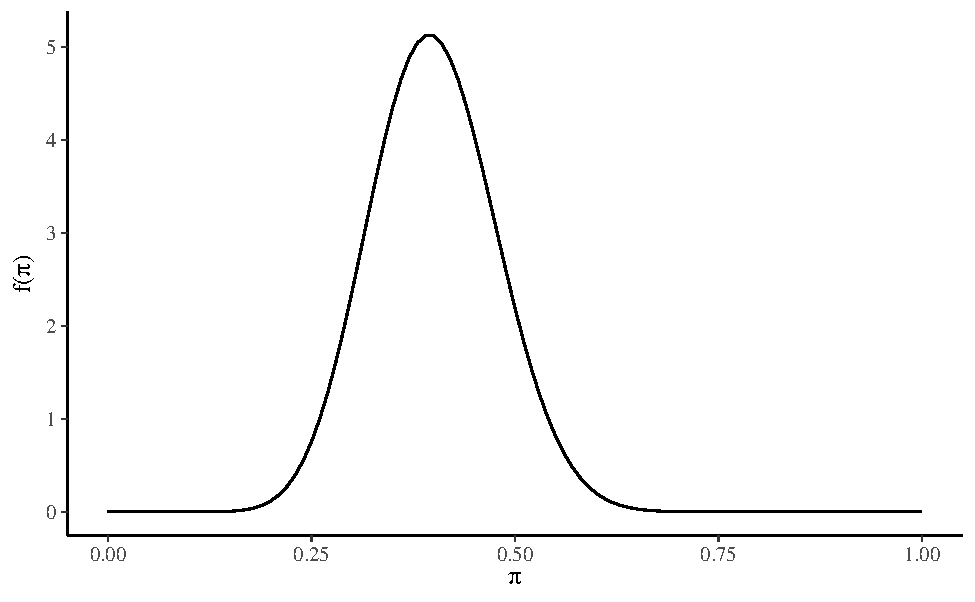
\includegraphics{ds4psy_files/figure-latex/unnamed-chunk-44-1} \end{center}

La media della distribuzione a priori diventa:

\begin{Shaded}
\begin{Highlighting}[]
\DecValTok{16} \SpecialCharTok{/}\NormalTok{ (}\DecValTok{16} \SpecialCharTok{+} \DecValTok{24}\NormalTok{)}
\CommentTok{\#\textgreater{} [1] 0.4}
\end{Highlighting}
\end{Shaded}

e la moda è

\begin{Shaded}
\begin{Highlighting}[]
\NormalTok{(}\DecValTok{16} \SpecialCharTok{{-}} \DecValTok{1}\NormalTok{) }\SpecialCharTok{/}\NormalTok{ (}\DecValTok{16} \SpecialCharTok{+} \DecValTok{24} \SpecialCharTok{{-}} \DecValTok{2}\NormalTok{)}
\CommentTok{\#\textgreater{} [1] 0.3947}
\end{Highlighting}
\end{Shaded}

Inoltre, la deviazione standard della distribuzione a priori diventa

\begin{Shaded}
\begin{Highlighting}[]
\FunctionTok{sqrt}\NormalTok{((}\DecValTok{16} \SpecialCharTok{*} \DecValTok{24}\NormalTok{) }\SpecialCharTok{/}\NormalTok{ ((}\DecValTok{16} \SpecialCharTok{+} \DecValTok{24}\NormalTok{)}\SpecialCharTok{\^{}}\DecValTok{2} \SpecialCharTok{*}\NormalTok{ (}\DecValTok{16} \SpecialCharTok{+} \DecValTok{24} \SpecialCharTok{+} \DecValTok{1}\NormalTok{)))}
\CommentTok{\#\textgreater{} [1] 0.07651}
\end{Highlighting}
\end{Shaded}

uguale a circa 8 punti percentuali. Verifichiamo:

\begin{Shaded}
\begin{Highlighting}[]
\NormalTok{bayesrules}\SpecialCharTok{::}\FunctionTok{summarize\_beta}\NormalTok{(}\AttributeTok{alpha =} \DecValTok{16}\NormalTok{, }\AttributeTok{beta =} \DecValTok{24}\NormalTok{)}
\CommentTok{\#\textgreater{}   mean   mode      var      sd}
\CommentTok{\#\textgreater{} 1  0.4 0.3947 0.005854 0.07651}
\end{Highlighting}
\end{Shaded}

Questo significa che le nostre credenze a priori rispetto la possibilità di recidiva tendono a deviare di circa 8 punti percentuali rispetto alla media della distribuzione a priori che corrisponde circa a 0.40.
\end{exercise}

\hypertarget{distribuzione-di-cauchy}{%
\section{Distribuzione di Cauchy}\label{distribuzione-di-cauchy}}

La distribuzione di Cauchy è un caso speciale della distribuzione di \(t\) di Student con 1 grado di libertà. È definita da una densità di probabilità che corrisponde alla funzione, dipendente da due parametri \(\theta\) e \(d\) (con la condizione \(d > 0\)),

\begin{equation}
f(x; \theta, d) = \frac{1}{\pi d} \frac{1}{1 + \left(\frac{x - \theta}{d} \right)^2},
\end{equation}

dove \(\theta\) è la mediana della distribuzione e \(d\) ne misura la larghezza a metà altezza.

\hypertarget{distribuzione-log-normale}{%
\section{Distribuzione log-normale}\label{distribuzione-log-normale}}

Sia \(y\) una variabile casuale avente distribuzione normale con media \(\mu\) e varianza \(\sigma^2\). Definiamo poi una nuova variabile casuale \(x\) attraverso la relazione

\[
x = e^y \quad \Longleftrightarrow \quad y = \log x.
\] Il dominio di definizione della \(x\) è il semiasse \(x > 0\) e la densità di probabilità \(f(x)\) è data da

\begin{equation}
f(x) = \frac{1}{\sigma \sqrt{2 \pi}} \frac{1}{x} \exp \left\{-\frac{(\log x -  \mu)^2}{2 \sigma^2} \right\}.
\end{equation}

Questa funzione di densità si chiama log-normale.

Il valore atteso e la varianza di una distribuzione log-normale sono dati dalle seguenti equazioni:

\begin{equation}
\E(x) = \exp \left\{\mu + \frac{\sigma^2}{2} \right\}.
\end{equation}

\begin{equation}
\Var(x) = \exp \left\{2 \mu + \sigma^2 \right\} \left(\exp \left\{\sigma^2 \right\}  -1\right).
\end{equation}

Si può dimostrare che il prodotto di variabili casuali log-normali ed indipendenti segue una distribuzione log-normale.

\hypertarget{distribuzione-di-pareto}{%
\section{Distribuzione di Pareto}\label{distribuzione-di-pareto}}

La distribuzione paretiana (o distribuzione di Pareto) è una distribuzione di probabilità continua e così chiamata in onore di Vilfredo Pareto. La distribuzione di Pareto è una distribuzione di probabilità con legge di potenza utilizzata nella descrizione di fenomeni sociali e molti altri tipi di fenomeni osservabili. Originariamente applicata per descrivere la distribuzione del reddito in una società, adattandosi alla tendenza che una grande porzione di ricchezza è detenuta da una piccola frazione della popolazione, la distribuzione di Pareto è diventata colloquialmente nota e indicata come il principio di Pareto, o ``regola 80-20''. Questa regola afferma che, ad esempio, l'80\% della ricchezza di una società è detenuto dal 20\% della sua popolazione. Viene spesso applicata nello studio della distribuzione del reddito, della dimensione dell'impresa, della dimensione di una popolazione e nelle fluttuazioni del prezzo delle azioni.

La densità di una distribuzione di Pareto è

\[
f(x)=(x_m/x)^\alpha,
\]

dove \(x_m\) (parametro di scala) è il minimo (necessariamente positivo) valore possibile di \(X\) e \(\alpha\) è un parametro di forma.

\begin{center}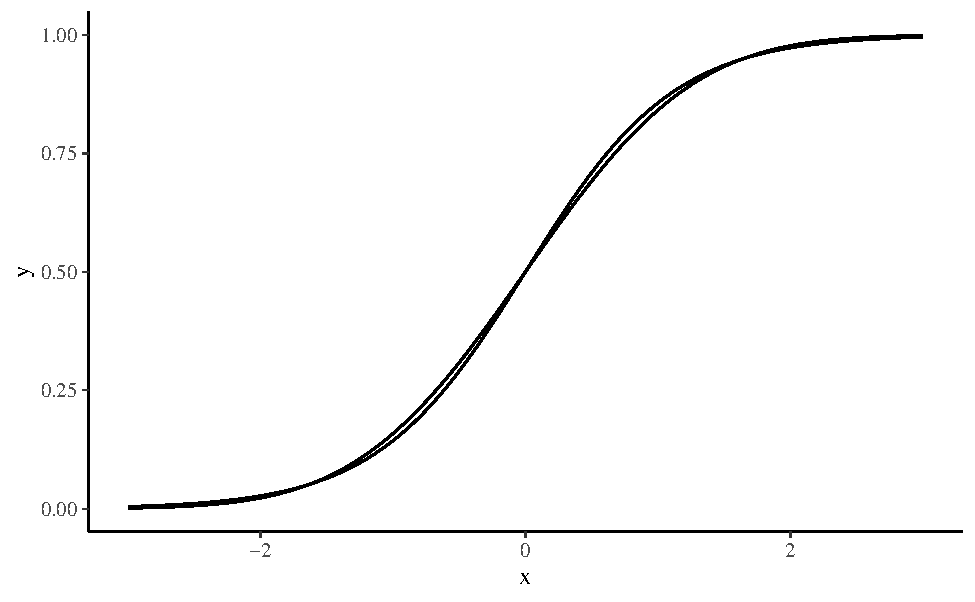
\includegraphics{ds4psy_files/figure-latex/unnamed-chunk-49-1} \end{center}

\noindent La distribuzione di Pareto ha una asimmetria positiva. Il supporto della distribuzione di Pareto è la retta reale positiva. Tutti i valori devono essere maggiori del parametro di scala \(x_m\), che è in realtà un parametro di soglia.

\hypertarget{appendix:bayes-updating}{%
\chapter{Aggiornamento Bayesiano}\label{appendix:bayes-updating}}

Per fornire un esempio di aggiornamento bayesiano, consideriamo il seguente problema. Supponiamo che, per qualche strano errore di produzione, una fabbrica produca due tipi di monete. Il primo tipo di monete ha la caratteristica che, quando una moneta viene lanciata, la probabilità di osservare l'esito ``testa'' è 0.6. Per semplicità, sia \(\theta\) la probabilità di osservare l'esito ``testa''. Per una moneta del primo tipo, dunque, \(\theta = 0.6\). Per una moneta del secondo tipo, invece, la probabilità di produrre l'esito ``testa'' è 0.4. Ovvero, \(\theta = 0.4\).

Noi possediamo una moneta, ma non sappiamo se è del primo tipo o del secondo tipo. Sappiamo solo che il 75\% delle monete sono del primo tipo e il 25\% sono del secondo tipo. Sulla base di questa conoscenza \emph{a priori} -- ovvero sulla base di una conoscenza ottenuta senza avere eseguitol'esperimento che consiste nel lanciare la moneta una serie di volte per osservare gli esiti prodotti -- possiamo dire che la probabilità di una prima ipotesi, secondo la quale \(\theta = 0.6\), è 3 volte più grande della probabilità di una seconda ipotesi, secondo la quale \(\theta = 0.4\). Senza avere eseguito alcun esperimento casuale con la moneta, questo è quello che sappiamo.

Ora immaginiamo di lanciare una moneta due volte e di ottenere il risultato seguente: \(\{T, C\}\). Quello che ci chiediamo è: sulla base di questa evidenza, come cambiano le probabilità che associamo alle due ipotesi? In altre parole, ci chiediamo qual è la probabilità di ciascuna ipotesi alla luce dei dati che sono stati osservati: \(P(H \mid y)\), laddove \(y\) sono i dati osservati. Tale probabilità si chiama probabilità a posteriori. Inoltre, se confrontiamo le due ipotesi, ci chiediamo quale valore assuma il rapporto \(\frac{P(H_1 \mid y)}{P(H_2 \mid y)}\). Tale rapporto ci dice quanto è più probabile \(H_1\) rispetto ad \(H_2\), alla luce dei dati osservati. Infine, ci chiediamo come cambia il rapporto definito sopra, quando osserviamo via via nuovi risultati prodotti dal lancio della moneta.

Definiamo il problema in maniera più chiara. Conosciamo le probabilità a priori, ovvero \(P(H_1) = 0.75\) e \(P(H_1) = 0.25\). Quello che vogliamo conoscere sono le probabilità a posteriori \(P(H_1 \mid y)\) e \(P(H_2 \mid y)\). Per trovare le probabilità a posteriori applichiamo il teorema di Bayes:

\[
\begin{split}
P(H_1 \mid y) &= \frac{P(y \mid H_1) P(H_1)}{P(y)} \\
&= \frac{P(y \mid H_1) P(H_1)}{P(y \mid H_1) P(H_1) + P(y \mid H_2) P(H_2)},
\end{split}
\]

laddove lo sviluppo del denominatore deriva da un'applicazione del teorema della probabilità totale. Inoltre,

\[
P(H_2 \mid y) = \frac{P(y \mid H_2) P(H_2)}{P(y \mid H_1) P(H_1) + P(y \mid H_2) P(H_2)}.
\]

Se consideriamo l'ipotesi \(H_1\) = ``la probabilità di testa è 0.6'', allora la verosimiglianza dei dati \(\{T, C\}\), ovvero la probabilità di osservare questa specifica sequenza di T e C, è uguale a \(0.6 \times 0.4 = 0.24.\) Dunque, \(P(y \mid H_1) = 0.24\).

Se invece consideriamo l'ipotesi \(H_2\) = ``la probabilità di testa è 0.4'', allora la verosimiglianza dei dati \(\{T, C\}\) è \(0.4 \times 0.6 = 0.24\), ovvero, \(P(y \mid H_2) = 0.24\). In base alle due ipotesi \(H_1\) e \(H_2\), dunque, i dati osservati hanno la medesima plausibilità di essere osservati. Per semplicità, calcoliamo anche

\[
\begin{split}
P(y) &= P(y \mid H_1) P(H_1) + P(y \mid H_2) P(H_2) \\
&= 0.24 \cdot 0.75 + 0.24 \cdot 0.25 \\
&= 0.24.
\end{split}
\]

Le probabilità a posteriori diventano:

\[
\begin{split}
P(H_1 \mid y) &= \frac{P(y \mid H_1) P(H_1)}{P(y)}\\
&= \frac{0.24 \cdot 0.75}{0.24} \\
&= 0.75,
\end{split}
\]

\[
\begin{split}
P(H_2 \mid y) &= \frac{P(y \mid H_2) P(H_2)}{P(y)} \\
&= \frac{0.24 \cdot 0.25}{0.24} \\
&= 0.25.
\end{split}
\]

Possiamo dunque concludere dicendo che, sulla base dei dati osservati, l'ipotesi \(H_1\) ha una probabilità 3 volte maggiore di essere vera dell'ipotesi \(H_2\).

È tuttavia possibile raccogliere più evidenze e, sulla base di esse, le probabilità a posteriori cambieranno. Supponiamo di lanciare la moneta una terza volta e di osservare croce. I nostri dati dunque sono \(\{T, C, C\}\).

Di conseguenza, \(P(y \mid H_1) = 0.6 \cdot 0.4 \cdot 0.4 = 0.096\) e \(P(y \mid H_2) = 0.4 \cdot 0.6 \cdot 0.6 = 0.144\). Ne segue che le probabilità a posteriori diventano:

\[
\begin{split}
P(H_1 \mid y) &= \frac{P(y \mid H_1) P(H_1)}{P(y)} \\
&= \frac{0.096 \cdot 0.75}{0.096 \cdot 0.75 + 0.144 \cdot 0.25} \\
&= 0.667,
\end{split}
\]

\[
\begin{split}
P(H_2 \mid y) &= \frac{P(y \mid H_2) P(H_2)}{P(y)} \\
&= \frac{0.144 \cdot 0.25}{0.096 \cdot 0.75 + 0.144 \cdot 0.25} \\
&= 0.333.
\end{split}
\]

In queste circostanze, le evidenze che favoriscono \(H_1\) nei confronti di \(H_2\) sono solo pari ad un fattore di 2.

Se otteniamo ancora croce in un quarto lancio della moneta, i nostri dati diventano: \(\{T, C, C, C\}\). Ripetendo il ragionamento fatto sopra, \(P(y \mid H_1) = 0.6 \cdot 0.4 \cdot 0.4 \cdot 0.4 = 0.0384\) e \(P(y \mid H_2) = 0.4 \cdot 0.6 \cdot 0.6 \cdot 0.6 = 0.0864\). Dunque

\begin{equation}
P(H_1 \mid y) = \frac{0.0384 \cdot 0.75}{0.0384 \cdot 0.75 + 0.0864 \cdot 0.25} = 0.571,\notag
\end{equation}

\begin{equation}
P(H_2 \mid y) = \frac{0.0864 \cdot 0.25}{0.0384 \cdot 0.75 + 0.0864 \cdot 0.25} = 0.429.\notag
\end{equation}

e le evidenze a favore di \(H_1\) si riducono a 1.33. Se si ottenesse un altro esito croce in un sesto lancio della moneta, l'ipotesi \(H2\) diventerebbe più probabile dell'ipotesi \(H_1\).

In conclusione, questo esercizio ci fa capire come sia possibile aggiornare le nostre credenze sulla base delle evidenze disponibili, ovvero come sia possibile passare da un grado di conoscenza del mondo a priori a una conoscenza a posteriori. Se prima di lanciare la moneta ritenevamo che l'ipotesi \(H_1\) fosse tre volte più plausibile dell'ipotesi \(H_2\), dopo avere osservato uno specifico campione di dati siamo giunti alla conclusione opposta. Il processo di aggiornamento bayesiano, dunque, ci fornisce un metodo per modificare il livello di fiducia in una data ipotesi, alla luce di nuove informazioni.

\hypertarget{appendix:exrc-abs-prob}{%
\chapter{Il teorema della probabilità totale}\label{appendix:exrc-abs-prob}}

\begin{exercise}
Consideriamo un'urna che contiene 5 palline rosse e 2 palline verdi. Due palline vengono estratte, una dopo l'altra. Vogliamo sapere la probabilità dell'evento ``la seconda pallina estratta è rossa''.

Lo spazio campionario è \(\Omega = \{RR, RV, VR, VV\}\). Chiamiamo \(R_1\) l'evento ``la prima pallina estratta è rossa'', \(V_1\) l'evento ``la prima pallina estratta è verde'', \(R_2\) l'evento ``la seconda pallina estratta è rossa'' e \(V_2\) l'evento ``la seconda pallina estratta è verde''. Dobbiamo trovare \(P(R_2)\) e possiamo risolvere il problema usando il teorema della probabilità assoluta \eqref{eq:prob-total-1b}:

\[
\begin{split}
P(R_2) &= P(R_2 \mid R_1) P(R_1) + P(R_2 \mid V_1)P(V_1)\\
&= \frac{4}{6} \cdot \frac{5}{7} + \frac{5}{6} \cdot \frac{2}{7} \\
&= \frac{30}{42} = \frac{5}{7}.
\end{split}
\]

Se la prima estrazione è quella di una pallina rossa, nell'urna restano 4 palline rosse e due verdi, dunque, la probabilità che la seconda estrazione produca una pallina rossa è uguale a 4/6. La probabilità di una pallina rossa nella prima estrazione è 5/7. Se la prima estrazione è quella di una pallina verde, nell'urna restano 5 palline rosse e una pallina verde, dunque, la probabilità che la seconda estrazione produca una pallina rossa è uguale a 5/6. La probabilità di una pallina verde nella prima estrazione è 2/7.
\end{exercise}

  \bibliography{refs.bib,book.bib,packages.bib}

\printindex

\end{document}
